\documentclass{article}

% NeurIPS 2025 formatting
%\usepackage{neurips_2025}
\usepackage[preprint]{neurips_2025}

% Additional packages
\usepackage[utf8]{inputenc} % allow utf-8 input
\usepackage{fontenc}    % use 8-bit T1 fonts
\usepackage{hyperref}       % hyperlinks
\usepackage{url}            % simple URL typesetting
\usepackage{booktabs}       % professional-quality tables
\usepackage{amsfonts}       % blackboard math symbols
\usepackage{nicefrac}       % compact symbols for 1/2, etc.
\usepackage{microtype}      % microtypography
\usepackage[usenames,dvipsnames]{xcolor}         % colors
\usepackage{amsmath,amssymb,amsthm}
\usepackage{enumitem}
\usepackage{geometry}
\usepackage{tikz}
\usepackage{graphicx}
\usetikzlibrary{arrows.meta,positioning,fit,backgrounds,calc}
\graphicspath{{./POC}}



%%%% Macros
\newcommand{\Loss}{\mathcal{L}}
\newcommand{\R}{\mathbb{R}}
\newcommand{\E}{\mathbb{E}}
\newcommand{\He}{\mathrm{He}}
% Comments: 
\newcommand{\giulia}[1]{{\color{ForestGreen}\textbf{Giulia:} #1}}
%\newcommand{\giulia}[1]{}

\usepackage[textsize=tiny]{todonotes}
% \usepackage{colortbl}

\newcommand{\mf}[1]{\todo[color=orange!30,size=\tiny]{MF: #1}}

%%%% Theorem environments
\newtheorem{definition}{Definition}[section]
\newtheorem{lemma}{Lemma}[section]
\newtheorem{proposition}{Proposition}[section]
\newtheorem{corollary}{Corollary}[section]
\newtheorem{remark}{Remark}[section]


\title{Barriers for Learning in an Evolving World: \\a Mathematical Understanding of Loss of Plasticity}

\author{%
  Amir Joudaki$^{1}$ \And
  Giulia Lanzillotta$^{1}$ \And
  Mohammad Samragh Razlighi$^{2}$ \And
  Iman Mirzadeh$^{2}$ \And
  Keivan Alizadeh$^{2}$ \And
  Thomas Hofmann$^{1}$ \And
  Mehrdad Farajtabar$^{2}$ \And
  Fartash Faghri$^{2}$ %\And
  %\vspace{-20pt}
  \\
  $^{1}$ETH Zürich
  $^{2}$Apple \\
  \texttt{amir.joudaki@inf.ethz.ch},
  \texttt{\{fartash, farajtabar\}@apple.com}
  %\texttt{\{amir.joudaki, giulia.lanzillotta, thomas.hofmann\}@inf.ethz.ch} \\
  %\texttt{\{fartash, m\_samraghrazlighi, imirzadeh, kalizadehvahid, m\_farajtabar\}@apple.com}
}

\begin{document}
\maketitle

% \begin{abstract}
% Standard deep learning models, typically trained via back-propagation, demonstrate remarkable success within the conventional two-phase paradigm: an extensive training phase conducted on a largely stationary dataset, followed by deployment where the model weights are frozen or only minimally adjusted \cite{dohare2024loss}. However, as highlighted by Richard Sutton and colleagues, this paradigm falters when models must continually interact with non-stationary environments \cite{dohare2024loss}. Over extended periods of learning in such settings, the very optimization process responsible for creating powerful representations can paradoxically undermine the network's capacity for future learning. Sutton terms this degradation \emph{loss of plasticity} \cite{dohare2024loss} . This work undertakes a first-principles investigation into the mechanisms underlying plasticity loss in gradient-based models. We propose a formal definition grounded in dynamical systems theory, identifying stable sub-manifolds in the parameter space as traps for gradient trajectories. We analyze two specific mechanisms leading to such traps: frozen units arising from activation saturation and cloned-unit manifolds resulting from representational redundancy. Furthermore, we explore conditions under which architectural choices or perturbations can potentially prevent or mitigate this collapse. Our theoretical framework aims to unify disparate observations regarding learning dynamics within a coherent mathematical structure. Notably, our findings reveal a fundamental tension: properties often considered beneficial in the static, two-phase regime, such as low-rank representations or simplicity bias \cite{huh2022lowrank, papyan2020prevalence}, appear to contribute directly to the loss of plasticity in continual learning scenarios \cite{dohare2024loss}. By consolidating key propositions regarding the barriers to continuous learning, this work points towards critical areas for future research aimed at developing truly adaptive artificial intelligence.
% \end{abstract}

% new abstract 
\begin{abstract}
    Standard deep learning models excel when trained on stationary datasets but often falter in non-stationary environments where continuous adaptation is crucial. This paradigm struggle is significantly due to the degradation of future learning capacity, a phenomenon termed loss of plasticity (LoP). This work undertakes a first-principles investigation into the mechanisms underlying LoP in gradient-based models. We propose a formal definition of LoP grounded in dynamical systems theory, identifying stable sub-manifolds in the parameter space that act as traps for gradient trajectories. Our analysis details two specific mechanisms leading to such traps: frozen units arising from activation saturation and cloned-unit manifolds resulting from representational redundancy. Furthermore, we explore conditions under which architectural choices or targeted perturbations might prevent or mitigate this plasticity collapse. A core finding of our theoretical framework is the revelation of a fundamental tension: properties widely considered beneficial for generalization in static, two-phase  learning regimes \mf{two-phase learning regime may be waugue/undefined at this stage in abstract}, such as the emergence of low-rank representations or inherent simplicity biases, appear to directly contribute to LoP in continual learning scenarios. By mathematically characterizing these barriers, this work pinpoints critical representational properties that hinder continuous learning, providing a clear direction for developing truly adaptive artificial intelligence. \mf{Perhaps adding something like "analysis verified by experiments or numerical results. To emphsize it's not only a theory paper. But don't make it bold.}
\end{abstract}

\section{Introduction}

The extraordinary success of back-propagation in training deep neural networks often relies on two implicit, yet critical, assumptions: \mf{Or even maybe removing the bullet format and write plainly. Two indentation at the bending of intro and in the first page of paper may not look very good.}
\begin{enumerate}
    \item \textbf{Stationarity.} The data distribution encountered during training is assumed to be identical, or very similar, to the distribution faced during deployment. Consequently, adaptation after the initial training phase is often minimal or absent.
    \item \textbf{One-shot randomness.} Diversity and the potential for exploration are primarily introduced through a single random initialization of the network's parameters. Subsequent training involves specialization, but the initial source of variability is gradually overwritten or ``forgotten'' by the optimization process.
\end{enumerate}
These assumptions break down when an artificial \emph{agent} must operate and learn continuously within an environment characterized by changing dynamics or evolving task distributions. This scenario, often termed continual or lifelong learning, presents a significant challenge known as the stability-plasticity dilemma \cite{abraham2005memory}: the system must be stable enough to retain previously acquired knowledge, yet plastic enough to integrate new information effectively.

\giulia{I would consider citing: \citep{berariu2021plasticity,lyle2023understanding,kumar2024regenerative,dohare2023maintaining,sokar2023dormant,chaudhry2018riemannian,ash2020warmstarting,nikishin2022primacy,dohare2021continual}. I can add (some of) them in the text.\newline}
Empirically, standard deep networks subjected to long sequences of tasks or slowly drifting data streams often exhibit a decline in their learning capability, eventually performing no better than simpler, shallow models \cite{dohare2024loss}\giulia{Add here \citep{berariu2021plasticity,dohare2021continual,nikishin2022primacy}}. This phenomenon, termed loss of plasticity, is distinct from the more widely studied problem of catastrophic forgetting \cite{mccloskey1989catastrophic, ratcliff1990connectionist, french1999catastrophic}, where learning new information overwrites previously learned knowledge. Loss of plasticity refers specifically to the diminished ability to learn new information effectively over time. Common symptoms associated with this degradation include explosive growth in weight magnitudes and saturation of activation functions; the emergence of ``dead'' ReLU units, whose upstream parameters cease to update due to consistently zero gradients \cite{nair2010rectified}; a collapse in the effective rank of hidden layer representations, indicating reduced feature diversity \cite{papyan2020prevalence, huh2022lowrank}; and redundancy or diminishing contribution from components like attention heads or convolutional filters \giulia{Add here \citep{lyle2023understanding}. Also \citep{nikishin2022primacy} talk about increased weight norm, \citep{dohare2021continual, lyle2022understanding} talk about inactive features and \citep{kumar2020implicit,gulcehre2022empirical} talk about low-rank and "implicit regularization" -- all in the context of LoP}.


Sutton and colleagues argue compellingly that such failures are intrinsically linked to the back-propagation algorithm itself \cite{dohare2024loss}. They posit that gradient descent, optimized for transient, single-task learning, relies heavily on the initial random state for exploration, a resource that is consumed and not replenished during prolonged training. Their work demonstrates that standard deep learning methods can lose plasticity until they perform comparably to linear networks, and suggests that maintaining plasticity requires mechanisms beyond pure gradient descent, such as continually injecting diversity via methods like their proposed continual backpropagation.

\paragraph{Goal of this paper.}
Motivated by these observations, this paper revisits the dynamics of gradient descent and back-propagation through the lens of dynamical systems theory. We seek to answer the fundamental question:
\begin{quote}
\emph{What structural features inherent in gradient flow dynamics inevitably lead to the loss of plasticity, and how might we design algorithms or architectures capable of perpetual adaptation?}
\end{quote}
The central proposition advanced in this work is that the tendency of gradient-based optimization to favor low-rank or ``simple'' representations lies at the heart of plasticity loss. While properties like low effective rank and simplicity bias are often associated with improved generalization in the standard two-phase learning paradigm \cite{huh2022lowrank, papyan2020prevalence, zhang2017understanding}, we argue that these very properties become detrimental in continual learning settings. By reducing the effective dimensionality of the network's feature space, they limit its capacity to adapt to novel information, thus contributing to the loss of plasticity observed by \cite{dohare2024loss} \giulia{and others...}.

\section{Preliminaries: A Dynamical Systems Framework}
\label{sec:framework}

Let $\theta\in\Theta\subseteq\R^p$ represent the parameters of a neural network. We consider training on a stream of data $\{(x_t,y_t)\}_{t\ge0}$ using gradient descent or its stochastic variants. The objective is typically to minimize a loss function $\Loss(\theta)$. The learning dynamics can be idealized by the continuous-time gradient flow:
\begin{equation}
    \frac{d\theta(t)}{dt} \;=\; -\nabla_\theta\Loss\bigl(\theta(t)\bigr).
    \label{eq:grad_flow}
\end{equation}
This perspective allows us to analyze the trajectory of parameters $\theta(t)$ in the parameter space $\Theta$ as driven by the negative gradient in the loss landscape \cite{saxe2014exact}.

We introduce the concept of a loss of plasticity manifold to formalize the idea of gradient trajectories becoming trapped in lower-dimensional subspaces, thereby restricting future learning capacity.

\begin{definition}[Loss of plasticity manifold]
\label{def:lop}
A smooth sub-manifold $\mathcal{M}\subset\Theta$ induces loss of plasticity if the following conditions hold:
\begin{enumerate}[label=(\alph*)]
    \item \textbf{Tangency:} The gradient of the loss function is tangent to the manifold at every point on the manifold. That is, $\nabla_\theta\Loss(\theta)\in T_\theta\mathcal{M}$ for all $\theta\in\mathcal{M}$, where $T_\theta\mathcal{M}$ denotes the tangent space of $\mathcal{M}$ at $\theta$. This ensures that once the gradient flow enters $\mathcal{M}$, it remains within $\mathcal{M}$.
    \item \textbf{Stability type:} The curvature of the loss function in directions normal to the manifold determines its stability. Let $N_\theta\mathcal{M}$ be the normal space to $\mathcal{M}$ at $\theta$. The stability is characterized by the Hessian $\nabla_\theta^2\Loss(\theta)$: \vspace{-4pt}
        \begin{align}
        \text{Stable:}\; &\forall v\in N_\theta\mathcal{M}\setminus\{0\}: v^\top\nabla_\theta^2\Loss(\theta)v > 0; \label{eq:stable}\\
        \text{Unstable:}\; &\forall v\in N_\theta\mathcal{M}\setminus\{0\}: v^\top\nabla_\theta^2\Loss(\theta)v < 0; \label{eq:unstable}\\
        \text{Saddle:}\; &\exists v_1,v_2\in N_\theta\mathcal{M}:\; v_1^\top\nabla_\theta^2\Loss v_1>0,\; v_2^\top\nabla_\theta^2\Loss v_2<0. \label{eq:saddle}
        \end{align}
\end{enumerate}
If the gradient flow enters a \emph{stable} loss of plasticity manifold, it is confined to trajectories within that manifold and cannot escape through gradient descent alone. The network's adaptability is consequently reduced, effectively limited by the dimensionality of $\mathcal{M}$, $\dim\mathcal{M} < p$.
\end{definition}

\begin{remark}
If the conditions in Definition~\ref{def:lop} hold irrespective of the specific data distribution generating the loss $\Loss$, we refer to it as structural loss of plasticity, implying it arises from the network architecture and optimization dynamics themselves. If the conditions hold only locally, perhaps for a specific data distribution or near a particular parameter configuration $\theta^\star$, the loss is local.
\end{remark}

\begin{remark}
It is important to emphasize that the loss of plasticity sub-manifold $\mathcal{M}$ is defined as being embedded within the $p$-dimensional parameter space $\Theta$. This is distinct from the $(p+1)$-dimensional graph of the loss function, i.e., the set $\{(\theta, \mathcal{L}(\theta)) \mid \theta \in \Theta \}$. Consequently, the tangent space $T_\theta\mathcal{M}$ is intrinsic to the sub-manifold $\mathcal{M}$ itself, existing within $\Theta$. The condition $\nabla_\theta\mathcal{L}(\theta) \in T_\theta\mathcal{M}$ then signifies that the gradient vector (which also lives in $\Theta$) lies along $\mathcal{M}$, thereby confining the gradient-based dynamics to this sub-manifold.
\end{remark}

We recall standard definitions for clarity.

\begin{definition}[Feed-forward neural network]
A feed-forward neural network is defined by a directed acyclic graph $G=(V,E)$, where $V$ is the set of nodes (neurons), $E$ is the set of directed edges (connections), $V_{\text{in}} \subset V$ are the input nodes, and $V_{\text{out}} \subset V$ are the output nodes. The activation $h(v)$ of a node $v \in V$ is computed as:
\[
h(v)=
\begin{cases}
x_v, & \text{if } v\in V_{\text{in}},\\
f_v\!\left(\sum_{u\!\in\!\mathrm{in}(v)}w(u,v)\,h(u)\right), &\text{otherwise}.
\end{cases}
\]
Here, $x_v$ is the input value for input node $v$, $f_v$ is the activation function associated with node $v$, $\mathrm{in}(v)$ is the set of nodes with edges pointing to $v$, and $w(u,v) \in \R$ is the weight parameter associated with the edge from $u$ to $v$. The network's output is the vector of activations $h(V_{\text{out}})$.
\end{definition}

\begin{definition}
Given a loss function $\Loss(h(V_{\text{out}}),y)$ comparing the network output $h(V_{\text{out}})$ to a target $y$, the back-propagation algorithm computes gradients via error signals $\delta(v)$. Let $z(v) = \sum_{u\in\mathrm{in}(v)}w(u,v)h(u)$ be the pre-activation of node $v$. The error signal is defined recursively:
\[
\delta(v)=
\begin{cases}
\partial\Loss/\partial h(v), & \text{if } v\in V_{\text{out}},\\[4pt]
\displaystyle\sum_{u\in\mathrm{out}(v)}\delta(u)\,w(v,u)\,f'_u(z(u)), &\text{otherwise},
\end{cases}
\]
where $\mathrm{out}(v)$ is the set of nodes receiving input from $v$, and $f'_u$ is the derivative of the activation function $f_u$. The gradient of the loss with respect to a weight $w(u,v)$ is then given by $\partial\Loss/\partial w(u,v)=\delta(v)\,f'_v(z(v))\,h(u)$.\qedhere
\end{definition}

\section{Sufficient Conditions for Loss of Plasticity}
\label{sec:frozen}
\giulia{I would change the structure of this section. As it is now, it feels like an "incomplete" list of arbitrary conditions. I think we could instead present the results in the more general frame of "emergence of low-rank feature spaces". Then 3.2 is a general mechanism which explains this emergence and its stability. And the dead/saturated unit phenomenon is one specific instance of the redundancy case.}
We now identify specific mechanisms that can lead to the formation of stable loss of plasticity manifolds. 

\subsection{Frozen Units via Activation Saturation}

A well-known phenomenon in training neural networks, particularly those using activation functions like Sigmoid, Tanh, or even ReLU, is activation saturation. When the pre-activation input to a neuron falls into a region where the activation function's derivative is zero or near-zero, the gradients flowing back through that neuron vanish. 

\begin{proposition}
\label{prop:saturated}
Consider a neuron $v$ with activation $h_i$ computed as $h_v = f_v(z_v)$, where $z_v$ is the pre-activation. let $\Theta_{\text{up}}(v)$ denote the set of "immediate upstream" parameters, defined as ${\Theta_{\text{up}}(v):=\{w(u,v)\}_{u\in \text{in}(v)}}$. If the derivative of the activation function is zero, i.e.,
\(
\frac{\partial h_v}{\partial z_v} = f'_v(z_v) = 0
\)
for all data samples encountered during a phase of training, then the gradient of the loss $\Loss$ with respect to any parameter $\theta \in \Theta_{\text{up}}$ will also be zero:
\(
\frac{\partial\Loss}{\partial\theta} = 0.
\)
Consequently, these upstream parameters $\Theta_{\text{up}}$ will not be updated by any subsequent gradient-based optimization step.  The parameter trajectory becomes confined to a sub-manifold where these parameters are fixed, representing a stable loss of plasticity manifold (assuming the saturation persists).
\end{proposition}

The proof follows directly from the chain rule in back-propagation. The error signal $\delta(u)$ for any node $u$ upstream of $i$ involves terms containing $f'_i(z_i)$. If $f'_i(z_i)=0$, these terms become zero, halting gradient flow to $\Theta_{\text{up}}$. \giulia{I would add here a discussion (theoretical or with empirical measures) of the assumption that node saturation persists during optimization. How likely and widespread is it?}

Examples of this phenomenon are abundant \giulia{and widely observed in the literature}:
\begin{itemize}
    \item \textbf{Dead ReLUs:} ReLU units ($f(z) = \max(0, z)$) whose input $z$ is consistently negative will have $f'(z)=0$, preventing updates to their incoming weights \cite{nair2010rectified}. This is often exacerbated by large negative biases or high learning rates.
    \item \textbf{Sigmoid/Tanh Saturation:} For Sigmoid or Tanh units, if the magnitude of the pre-activation $|z|$ becomes large, the derivative approaches zero, effectively freezing upstream learning.
    \item \textbf{Softmax Dominance:} In a Softmax layer, if one logit becomes significantly larger than others, its corresponding probability approaches 1, and the gradients for its associated weights can diminish.
    \item \textbf{Vanishing Attention Weights:} If the weights determining the contribution of some attention heads become very small (e.g., through regularization or optimization dynamics), those heads may cease to contribute meaningfully, and their parameters may stop updating.
\end{itemize}
This mechanism provides a clear pathway to plasticity loss where parts of the network become unresponsive to new data due to the properties of the activation functions and the dynamics of training. \giulia{Maybe we should be more precise here. Can we quantify how much loss of plasticity a single dead unit brings? How many dead units can be "tolerated" before losing the ability to fit a task?}

\begin{figure}[h!]
    \centering
    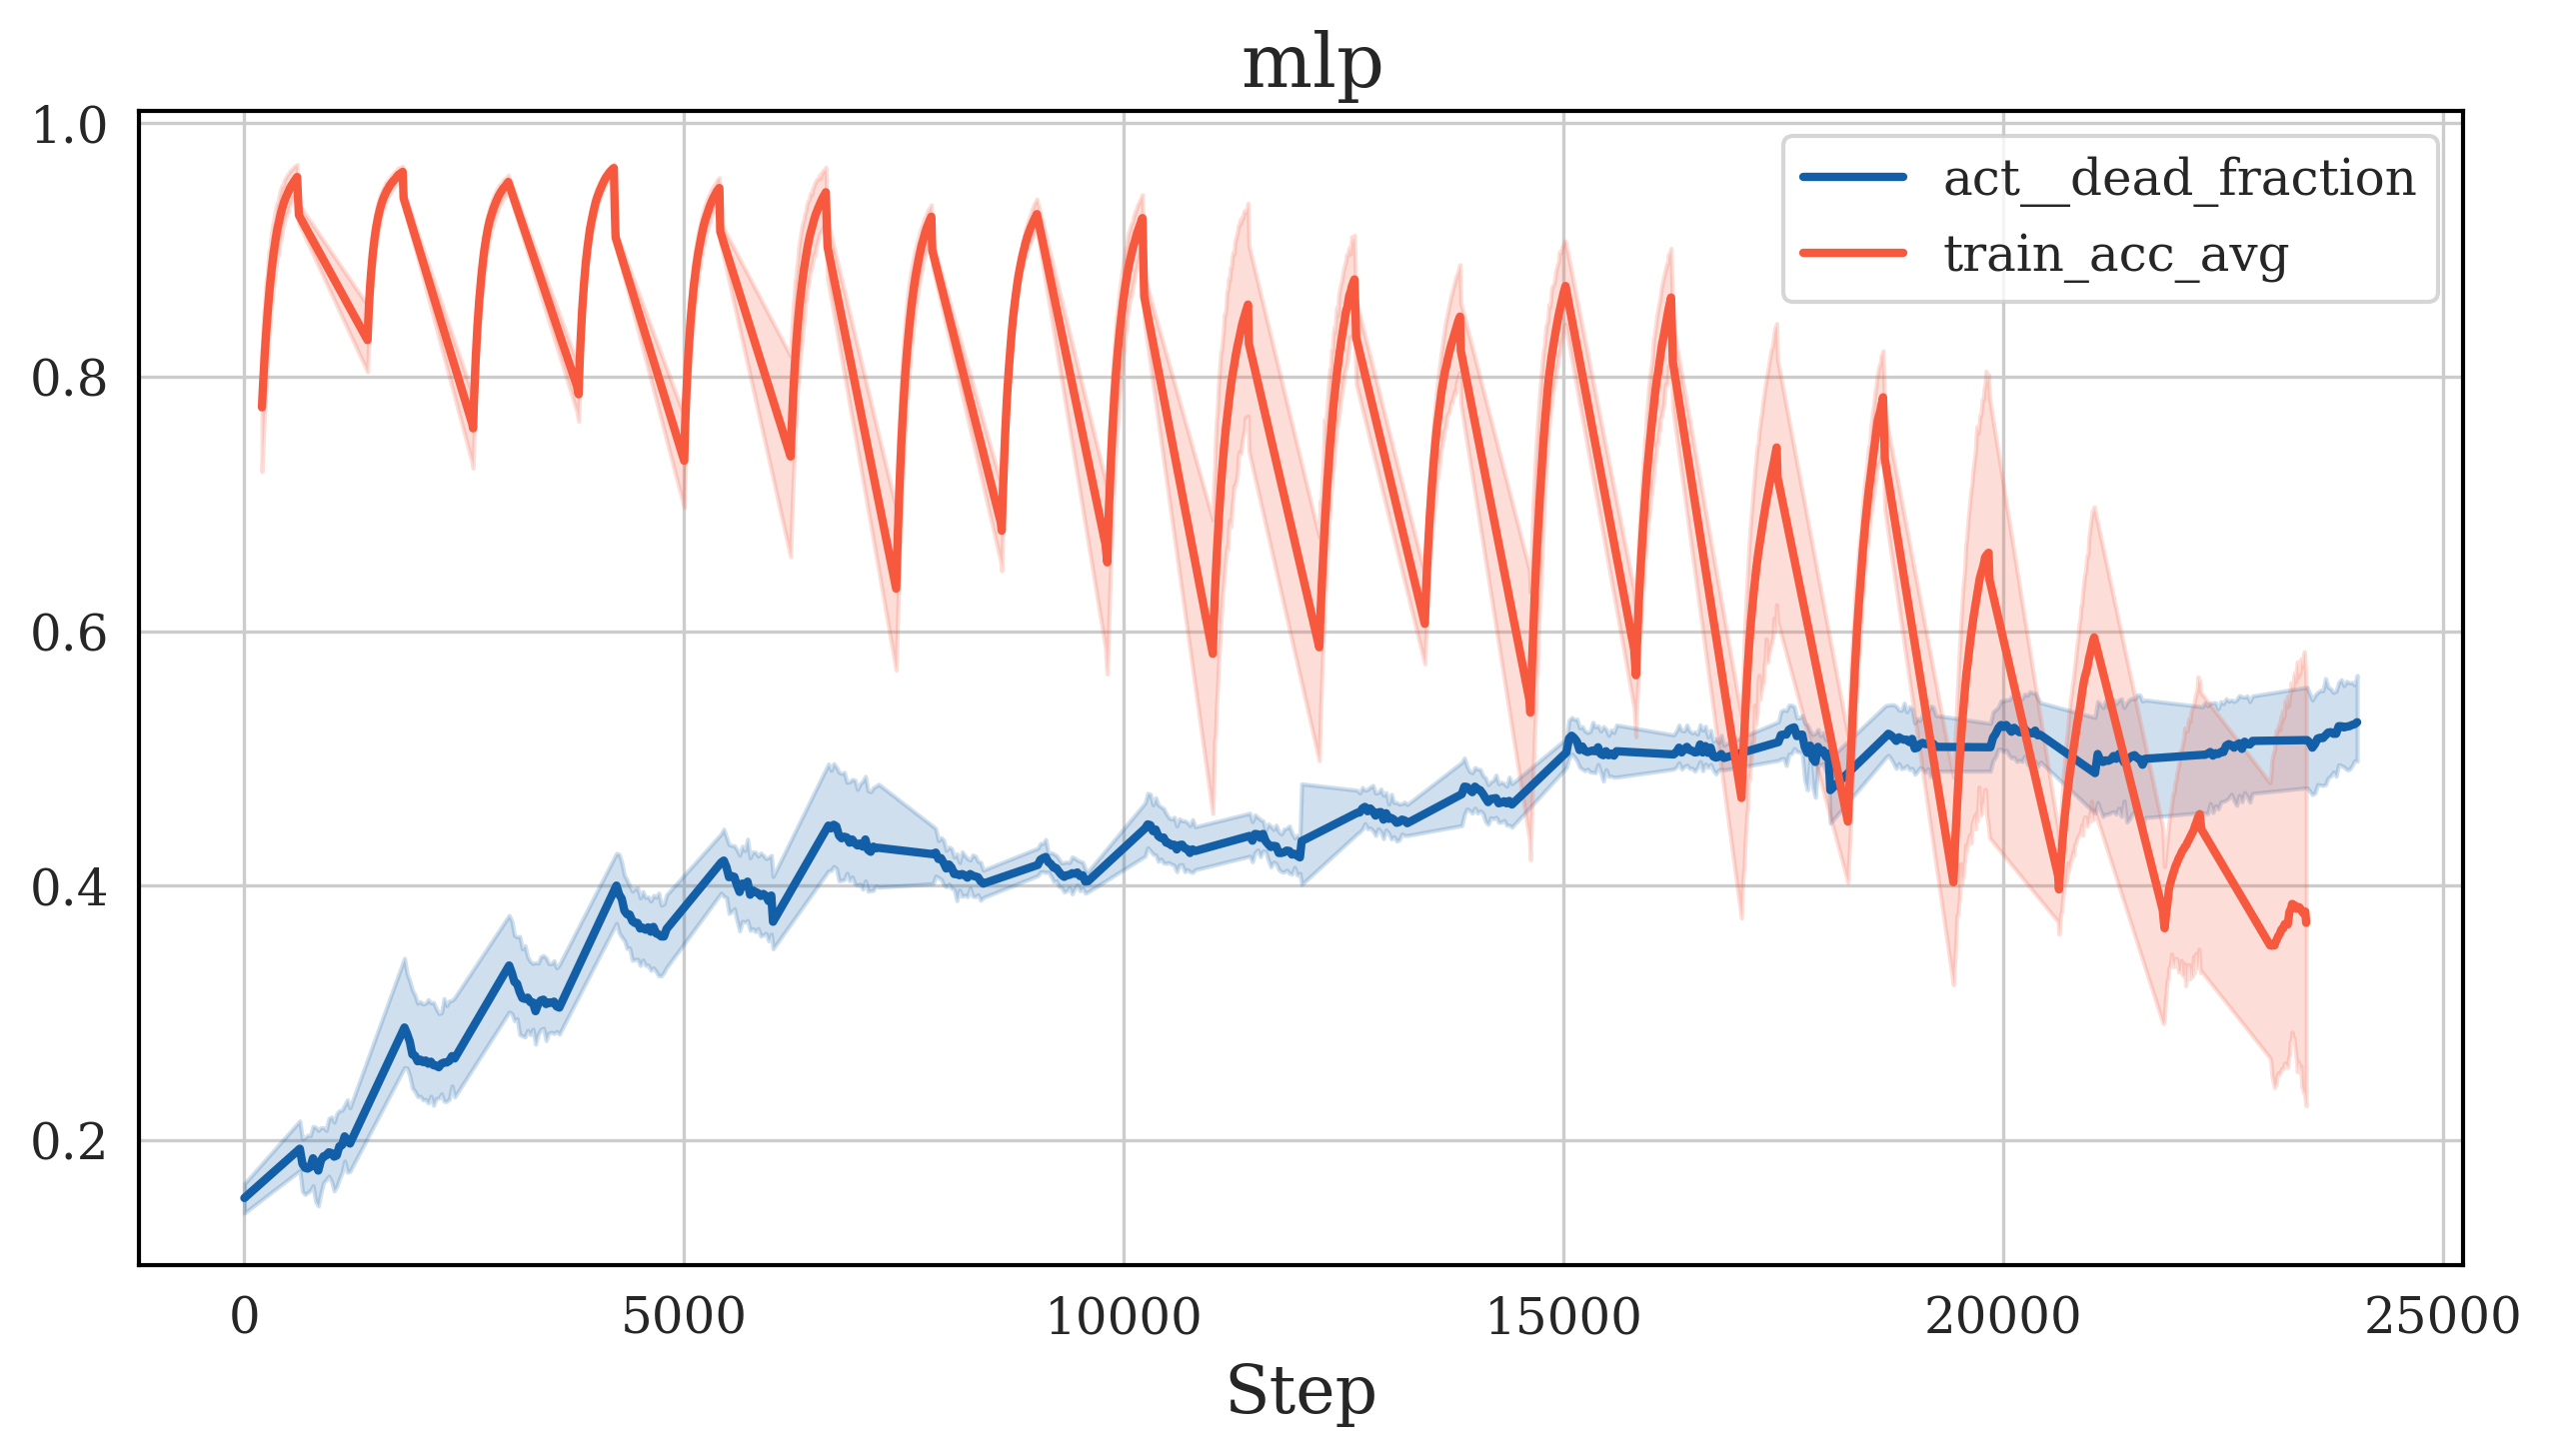
\includegraphics[width=0.4\linewidth]{paper/images/dead_frac_mlp.png}
    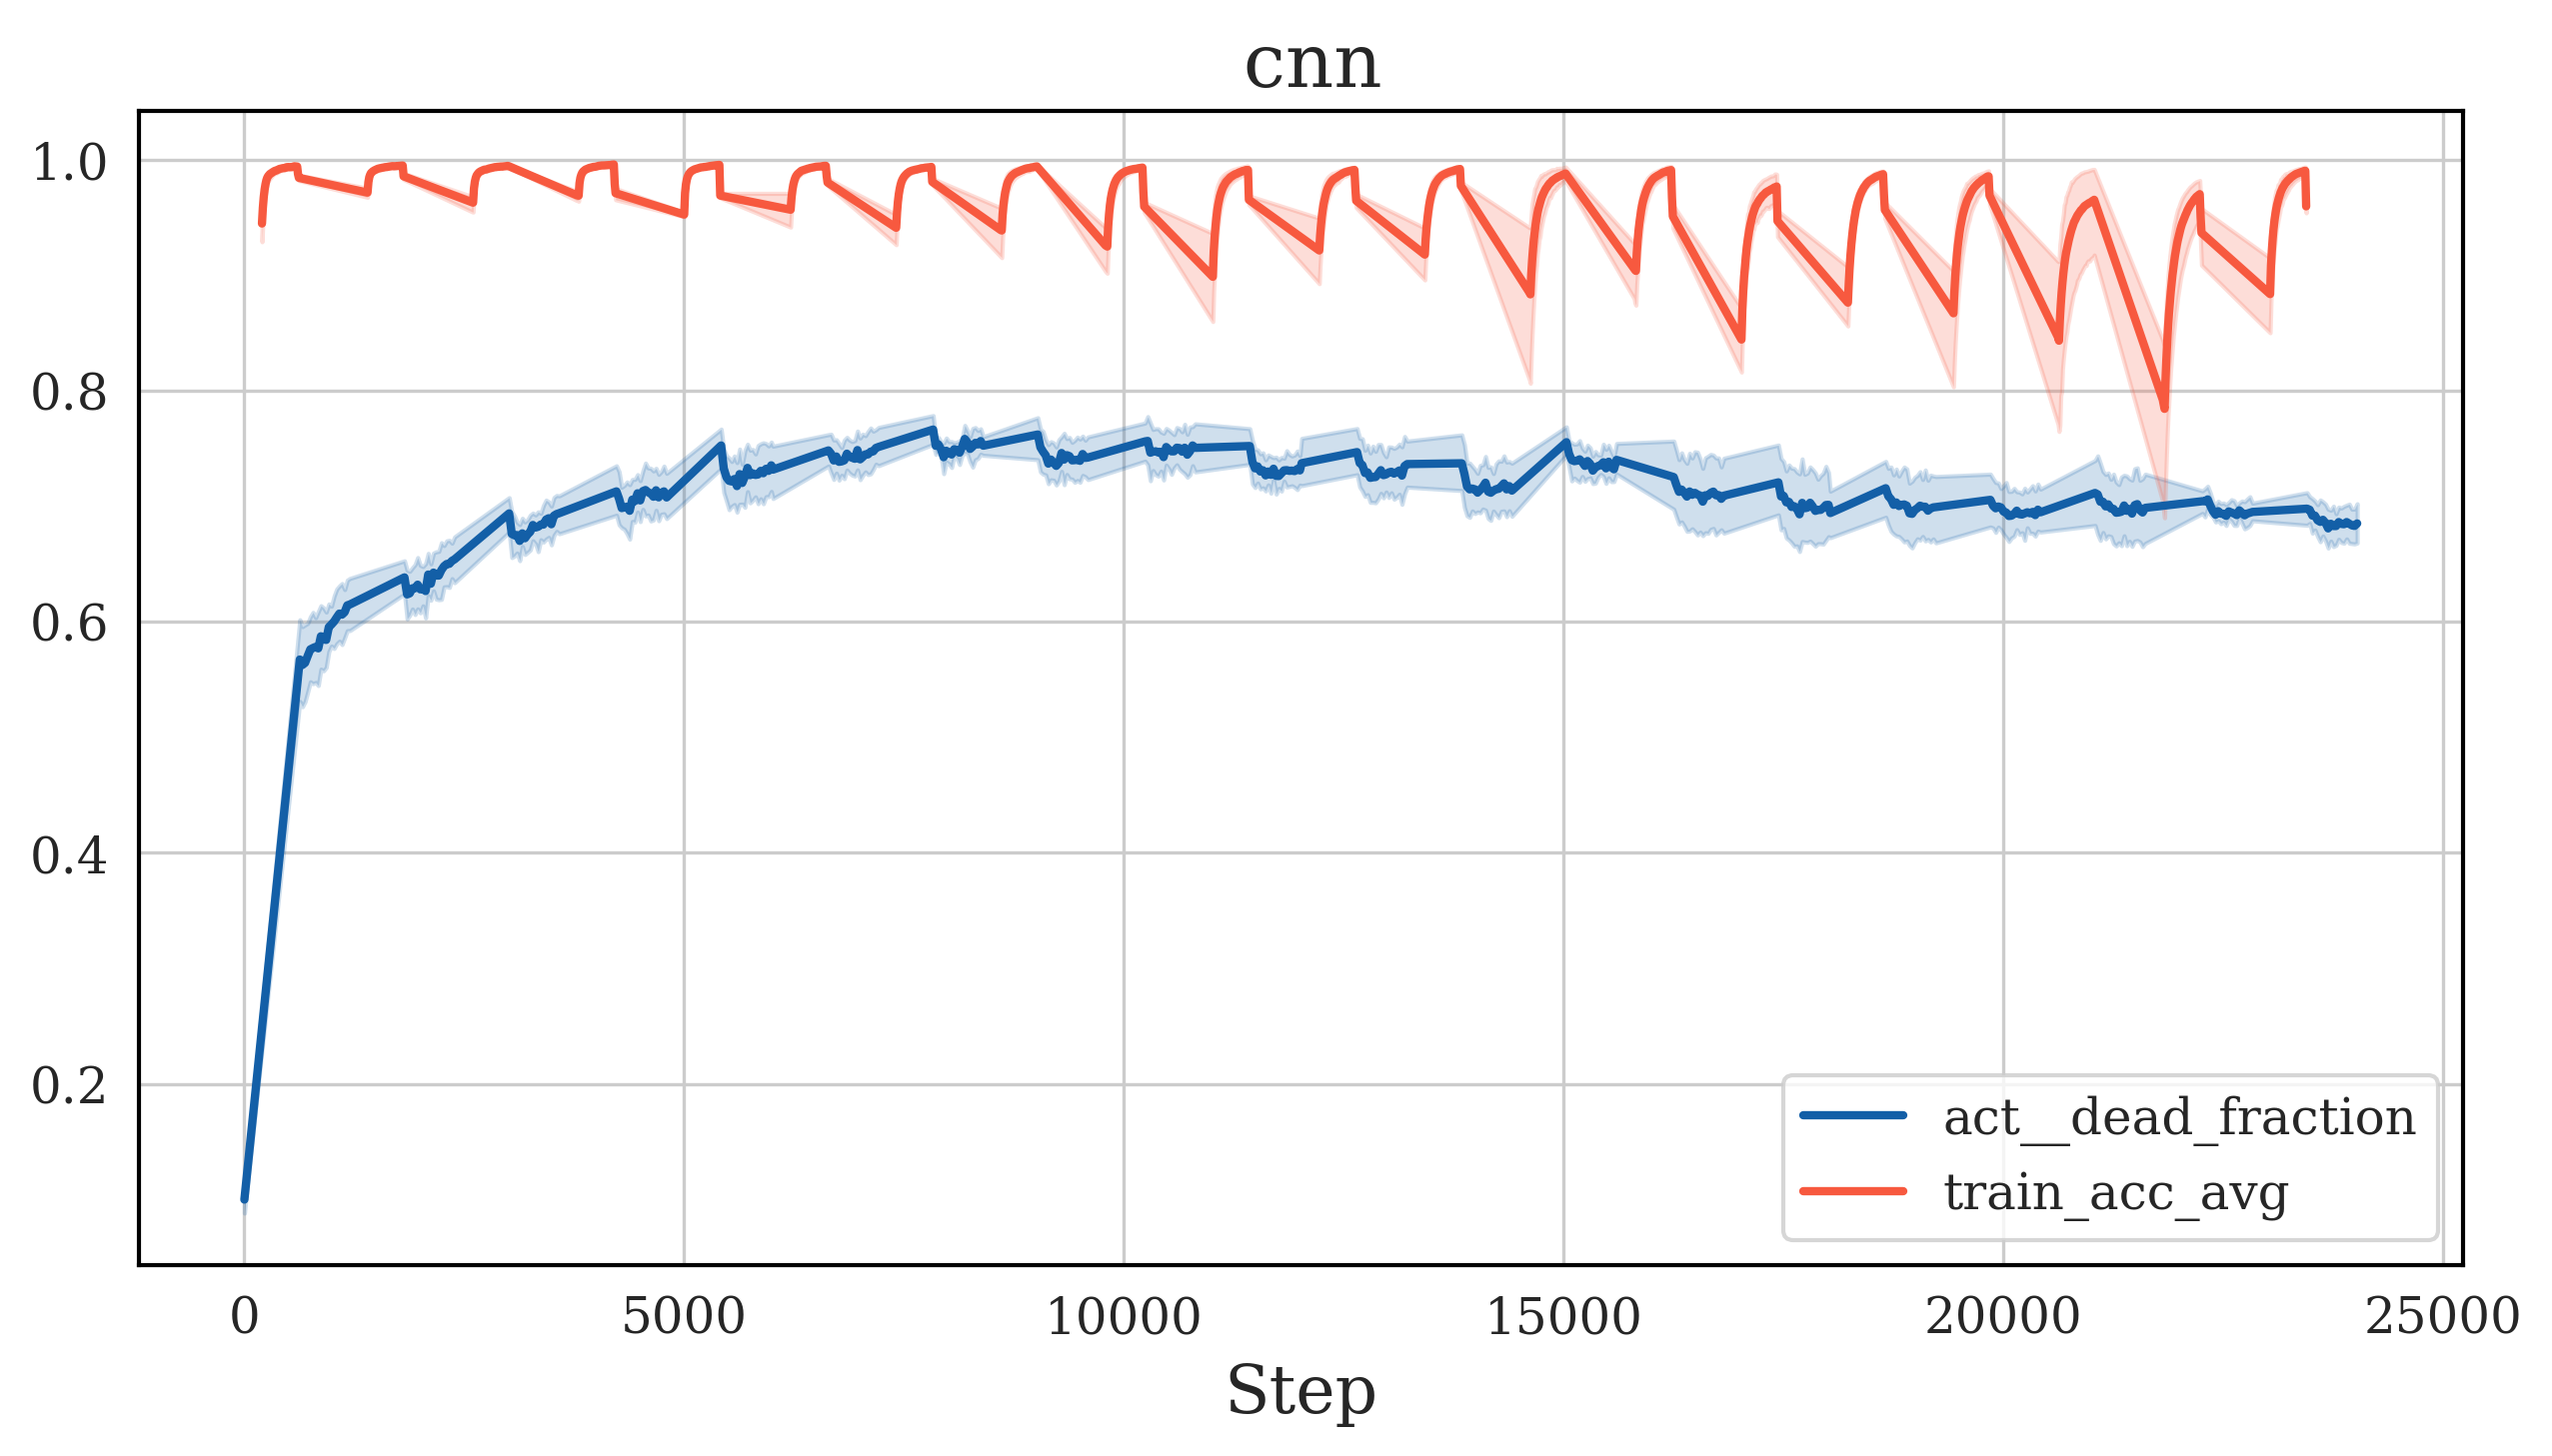
\includegraphics[width=0.4\linewidth]{paper/images/dead_frac_cnn.png}
    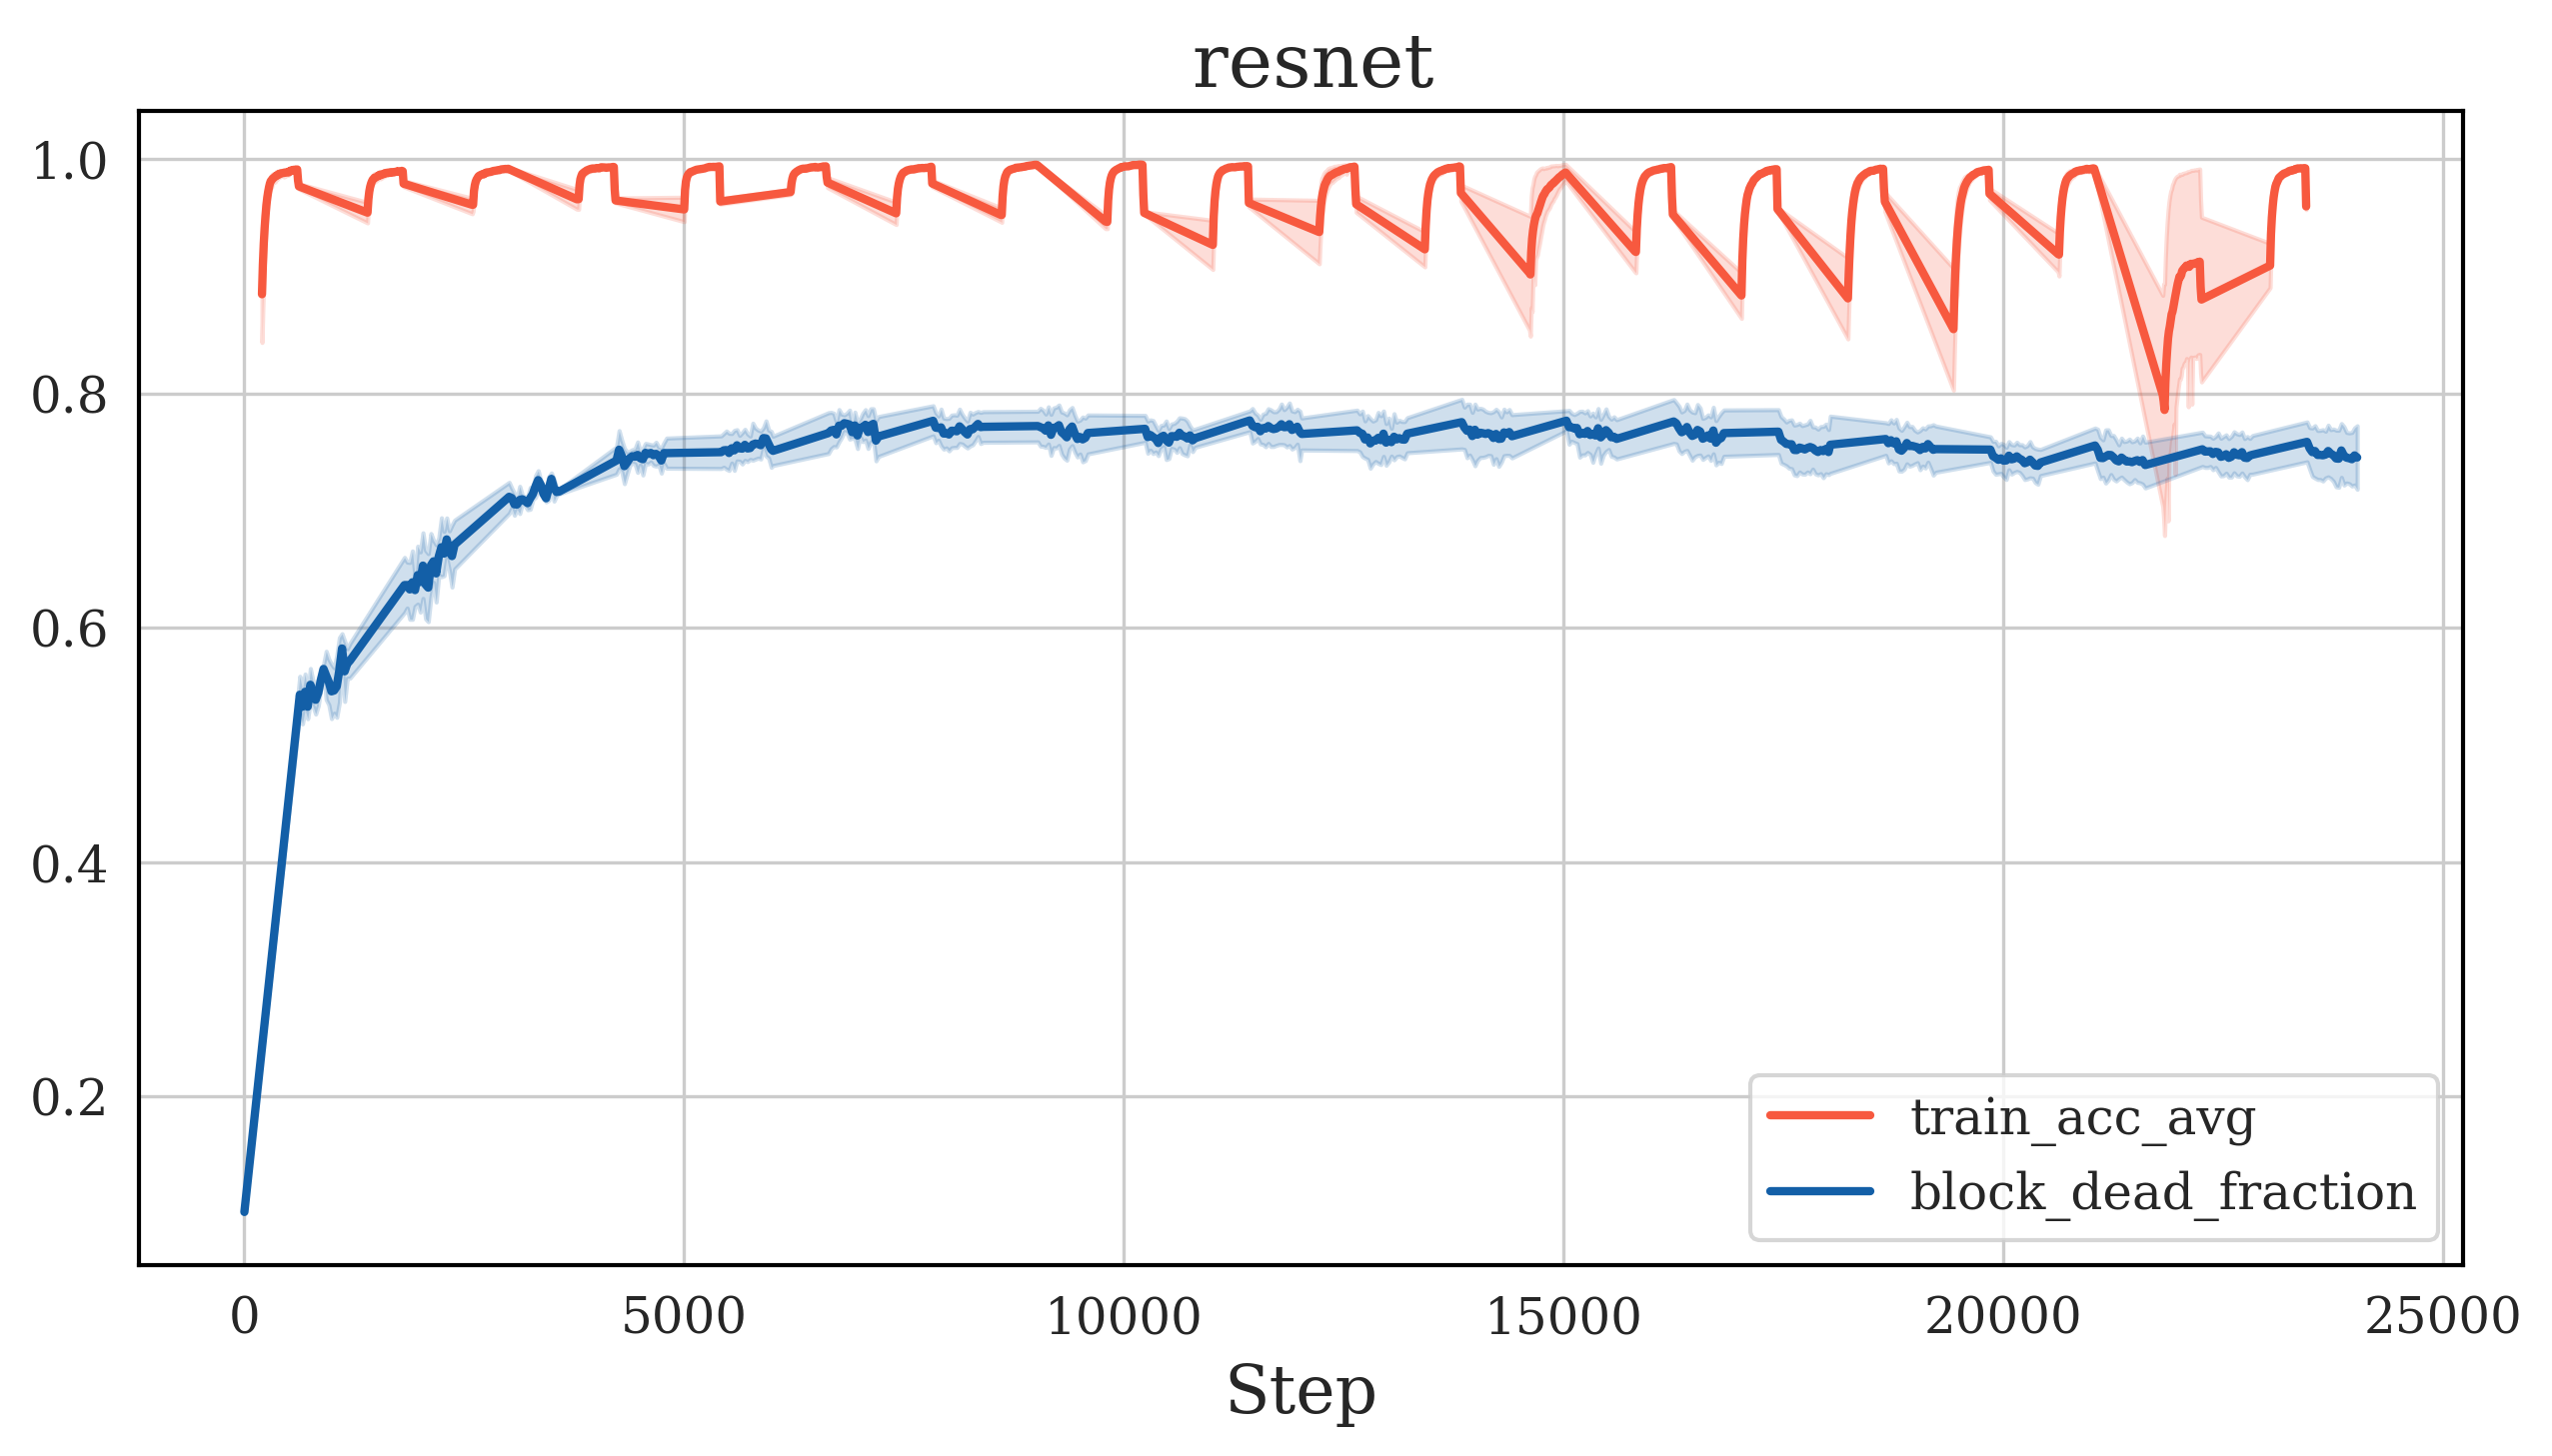
\includegraphics[width=0.4\linewidth]{paper/images/dead_frac_resnet.png}
    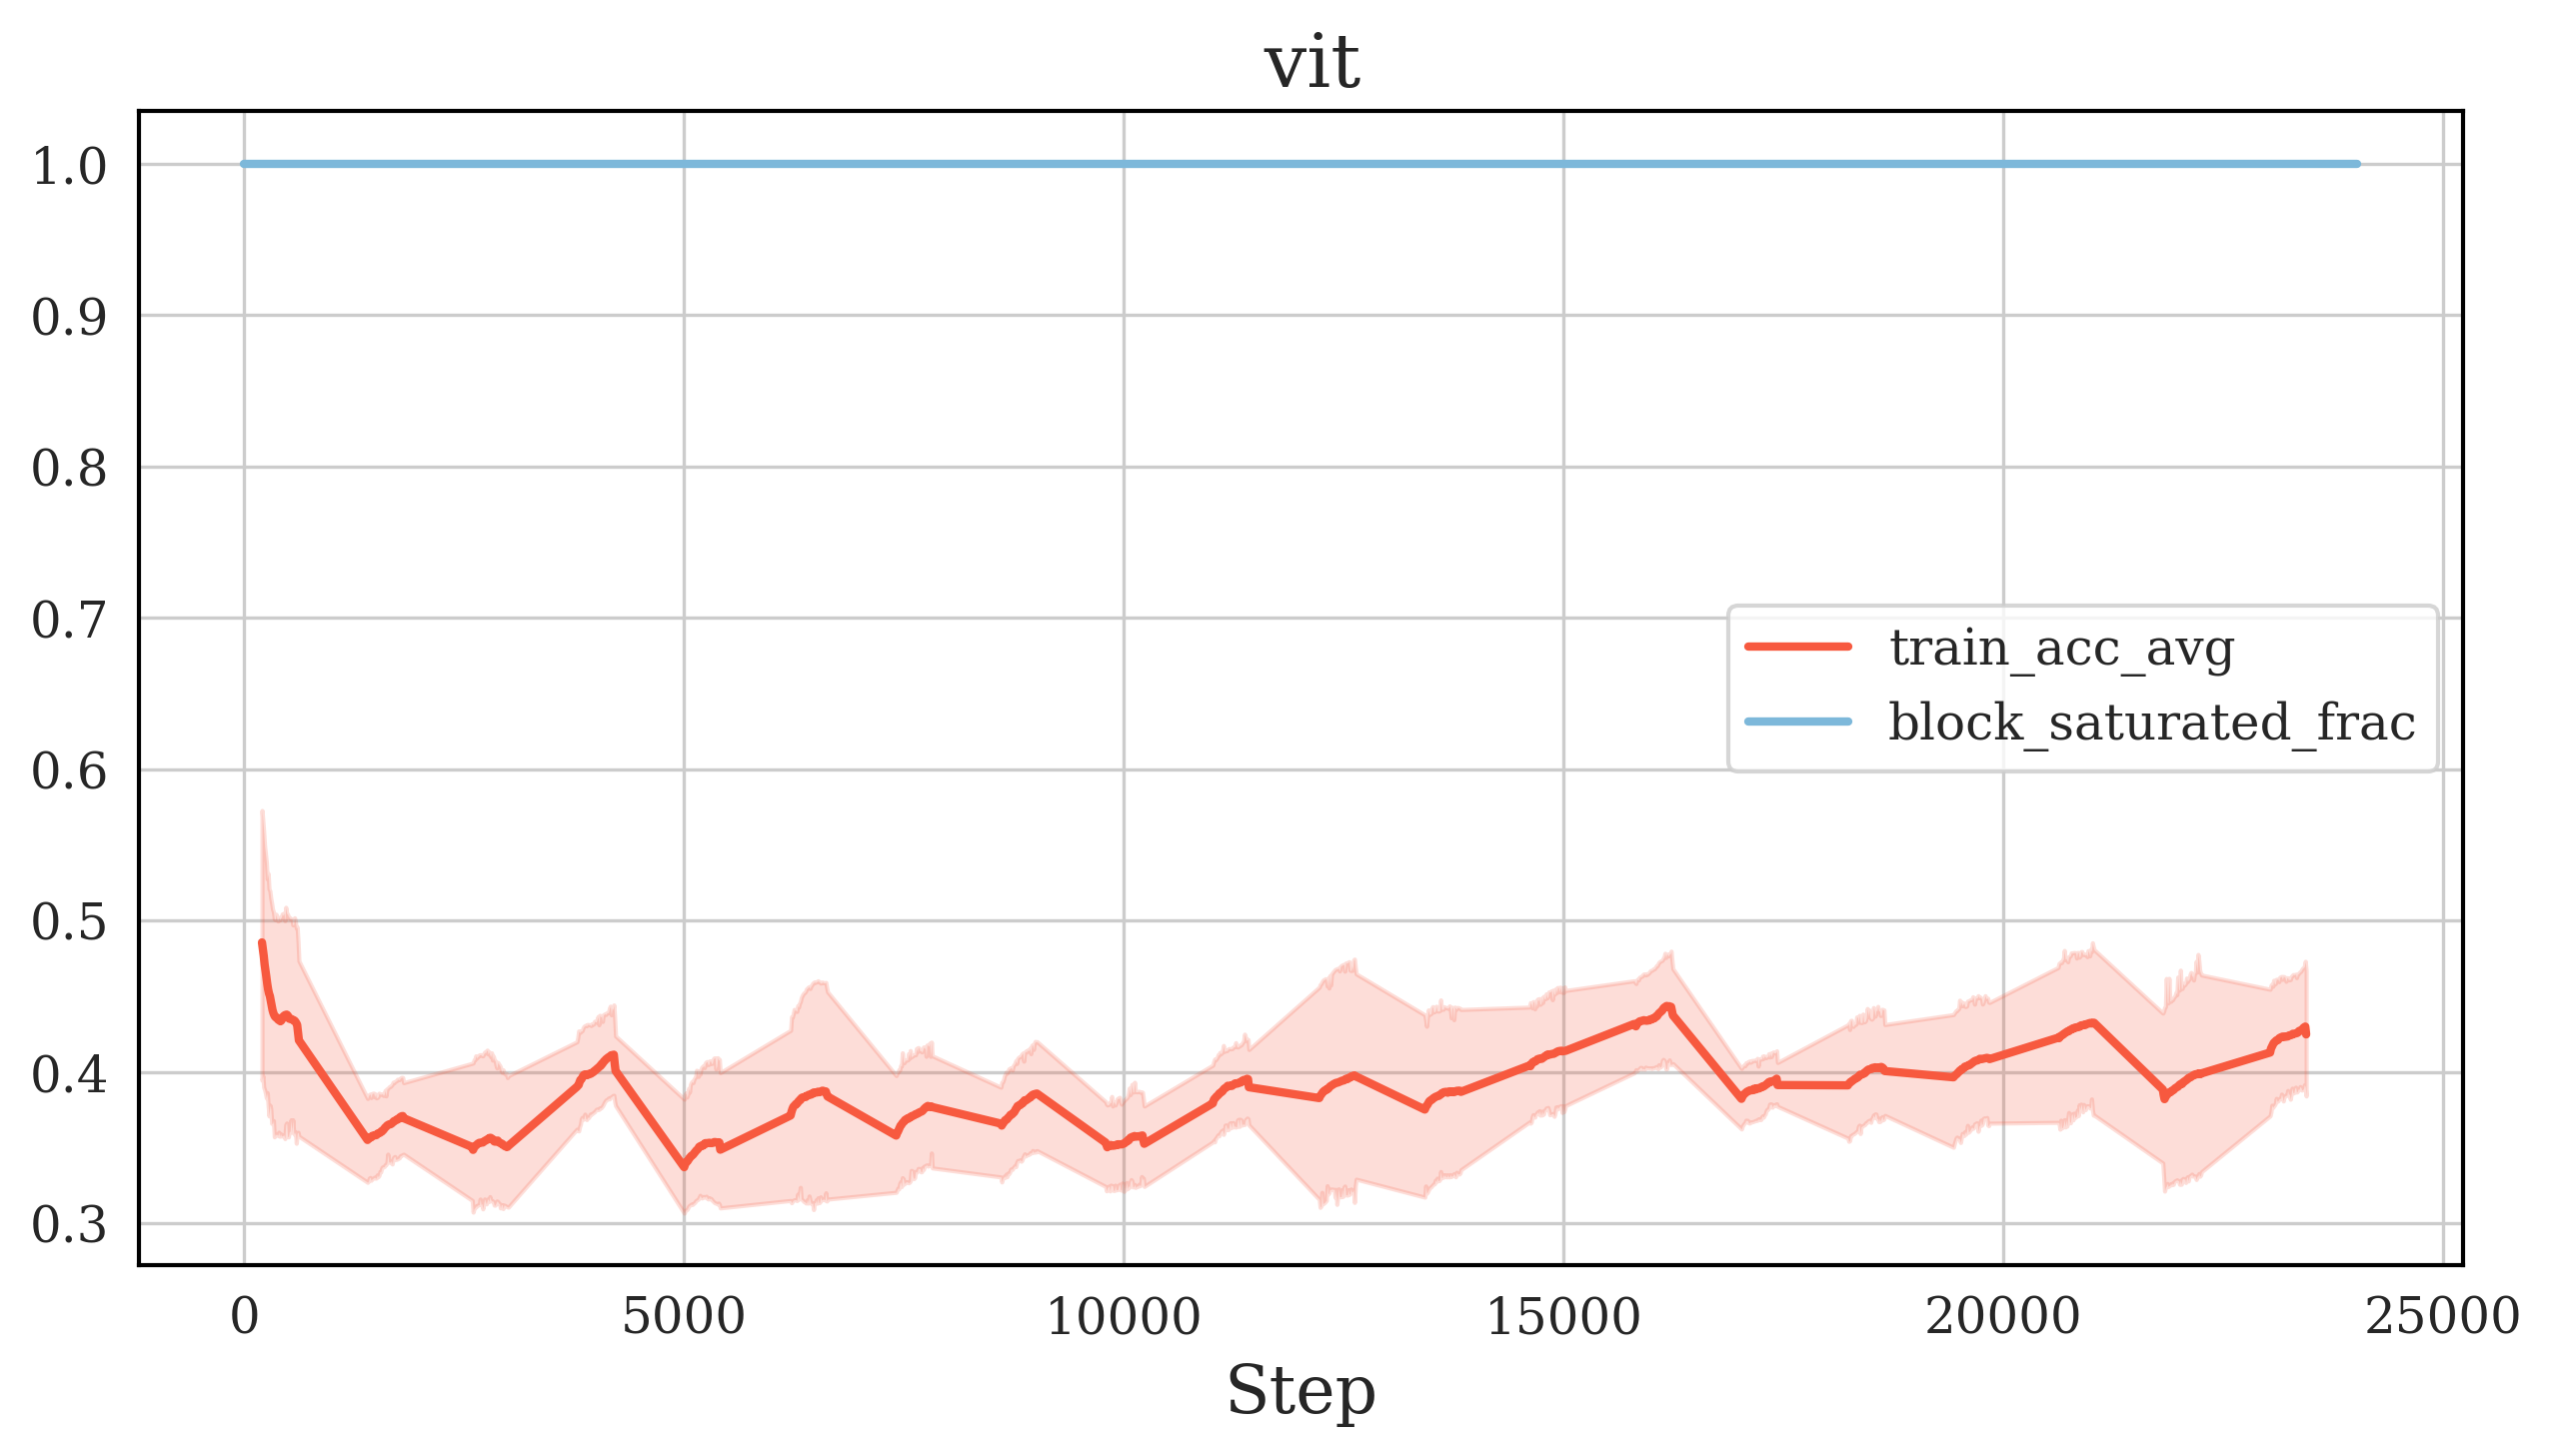
\includegraphics[width=0.4\linewidth]{paper/images/sat_frac_vit.png}
    
    \caption{(Placeholder figure, not final) No normalization and no dropout. The Accuracy is plotted as a rolling average, with window 20. For ViT we use layernorm.}
    \label{fig:DeadReLUs-LoP}
\end{figure}


\subsection{Cloned-Unit Manifolds via Redundancy}

Plasticity can also vanish even without explicit activation saturation if the network develops redundant representations, effectively behaving like a smaller network. This can happen in overparameterized models where multiple units or groups of units learn to perform identical functions.

To formally state the proposition, it is beneficial to define two more concepts related to matrix with bloock structure. 
\begin{definition}
    Suppose $X$ and $Y$ are adjacency matrices of respectively a graph with $n$ nodes and $m$ nodes, where $n < m$. A node covering is a set of disjoint sets  $\{S_1,\dots,S_m\},$ such that $\cup_{i\le m} S_i = \{1,\dots,n\}. $ These partitions defining blocks in $X$ matrix $X[S_i,S_j],$ where each block of $X$ corresponds to one element of $Y$.  We define the following block-wise properties: 
    \begin{itemize}
        \item Block-wise constant: all elements $X[S_i,S_j]$ are equal to $Y_{ij}.$
        \item Row-equitable: sum of every row in $X[S_i,S_j]$ is equal to $Y_{ij}.$
        \item Column-equitable: sum of every column in block $X[S_i,S_j]$ is equal to $Y_{ij}.$
    \end{itemize}
\end{definition}

\begin{proposition}
\label{prop:cloned}
    Let $G=(V,E,W)$ and $G=(\widetilde V,\widetilde E,\widetilde W)$
be, respectively, the \emph{base} and \emph{cloned} feed‑forward networks, with
weight parameters \(W=(w_{ij})_{(i,j)\in E}\) and
\(\widetilde{W}=(\widetilde w_{uv})_{(u,v)\in \widetilde E}\). Suppose there is a node covering of $\widetilde{G},$ such that blocks $(i,j)$ of $\widetilde{W}$ has row-sums and columns sums equal to $W_{i,j}.$ Under these conditions we have:
\begin{itemize}
    \item If two nodes are in the same partition $u,v \in S_i,$ they have similar forward and backward values: $h(v) = h(u)$ and $\delta(u)=\delta(v).$
    \item The gradient of the cloned network $\Delta\widetilde{W}$ is block-wise constant, with the block values equal to gradient of the smaller model $\Delta W$. Thus, adding the gradients will not change the row-sum or column sum equitability.
    \item If the network $\widetilde{G}$ is trained using gradient descent (or variants like SGD, Adam), then $\widetilde{W}_t - \widetilde{W}_0$ will always have a block-wise constant structure. In other words, the parameter trajectory $\widetilde{W}(t)$ starting from $\widetilde{W}_0$ will remain confined to a subspace of dimension of $W$. More specifically,
\end{itemize}
% A surjection
% \[
% \pi:\widetilde V\;\longrightarrow\;V,\qquad 
% S_i:=\pi^{-1}(i)\subset\widetilde V,
% \]
% satisfies \emph{forward-backward symmetry} (or simply
% \emph{clone conditions}) if for every pair of base neurons
% \((i,j)\in V\times V\) the following holds: 
% \begin{align}\label{eq:fbs}
%     \forall\,u\in S_i:\;
% \sum_{v\in S_j}\!\widetilde w_{uv}=w_{ij},
% \quad
% \forall\,v\in S_j:\;
% \sum_{u\in S_i}\!\widetilde w_{uv}=w_{ij}.
% \end{align}
% Under these conditions, if the network $\widetilde{G}$ is trained using gradient descent (or variants like SGD, Adam), the parameter trajectory $\widetilde{W}(t)$ starting from $\widetilde{W}_0$ will remain confined to an affine subspace. This subspace is defined by the initial weights plus changes that maintain the cloning structure, effectively parameterized by the smaller set of weights $W_t$ corresponding to the narrow network $G$. The dimension of this subspace is $|E|$, which is typically much smaller than the total number of parameters $|\widetilde{E}|$ in the cloned network.
% \(
% \widetilde{W}(t) \in \{\widetilde{W}_0 + \Delta\widetilde{W}(W_t) \mid W_t \text{ evolves according to } G \}.
% \)
\end{proposition}


% \begin{corollary}[Quotient graph formulation]
% \end{corollary}

This represents a form of \emph{structural} loss of plasticity, as the large network's dynamics are permanently constrained to mimic those of the smaller network, irrespective of the data distribution. \giulia{Here we need to work on providing an intuition of the proposition and the conditions which we require. At the moment it seems artificial.}

\paragraph{Insight into the proof via quotient graphs}: 

% \begin{proposition}[Cloned-unit plasticity loss]
% \label{prop:cloned}
% Consider a ``wide'' network $\widetilde{G}=(\widetilde{V},\widetilde{E},\widetilde{W})$ with parameters $\widetilde{W}$, and a ``base'' network $G=(V,E,W)$ with parameters $W$. Suppose there exists a surjection $\pi:\widetilde{V}\to V,$ which defines the partitions $S_u:=\{v\in \widetilde{V}: \pi(v)=\pi(u)\}.$ 
% \begin{enumerate}
%     \item The connectivity structure mirrors that of the base network: If there is an edge $(u,v) \in E$, then there are edges between nodes in $S_u$ and $S_v$ in $\widetilde{E}$, and vice-versa. Assume identical activation functions $f_v$ for all nodes within a partition $S_v$.
%     \item The initial weights $\widetilde{W}_0$ are set such that for any edge $(u,v) \in E$, the total incoming weight to any node $y \in S_v$ from partition $S_u$ is equal to the corresponding narrow network weight $W(u,v)$, and similarly for outgoing weights. Specifically, assume conditions such that forward activations and backward error signals are identical for all nodes within each partition $S_v$:
%     \begin{align}
%     % Simplified conceptual representation, formal conditions in proof
%     \sum_{b\in S_u} W(a,b)  = W(u,v) \quad \forall (u,v) \in E, a\in S_u.\\    \sum_{b\in S_u} W(a,b)  = W(u,v) \quad \forall (u,v) \in E, a\in S_u.\\
%     \end{align}
% \end{enumerate}
% Under these conditions, if the network $\widetilde{G}$ is trained using gradient descent (or variants like SGD, Adam), the parameter trajectory $\widetilde{W}(t)$ starting from $\widetilde{W}_0$ will remain confined to an affine subspace. This subspace is defined by the initial weights plus changes that maintain the cloning structure, effectively parameterized by the smaller set of weights $W_t$ corresponding to the narrow network $G$. The dimension of this subspace is $|E|$, which is typically much smaller than the total number of parameters $|\widetilde{E}|$ in the cloned network.
% \(
% \widetilde{W}(t) \in \{\widetilde{W}_0 + \Delta\widetilde{W}(W_t) \mid W_t \text{ evolves according to } G \}.
% \)
% This represents a form of \emph{structural} loss of plasticity, as the large network's dynamics are permanently constrained to mimic those of the smaller network, irrespective of the data distribution.
% \end{proposition}

The proof (detailed in Appendix~\ref{app:proofs}) relies on showing by induction that if activations $h(\cdot)$ and error signals $\delta(\cdot)$ are identical across nodes within each partition at one time step, they remain identical after a gradient update, provided the initial weights satisfy the cloning conditions. This implies that the gradients themselves exhibit this cloned structure, confining updates to the lower-dimensional manifold. This phenomenon is related to observations of symmetry and redundancy in deep networks, and connects to concepts like neural collapse where representations degenerate \cite{papyan2020prevalence} and simplicity bias where networks favor lower-complexity solutions \cite{huh2022lowrank}.

\begin{figure}[t]
    \centering
    \resizebox{\textwidth}{!}{
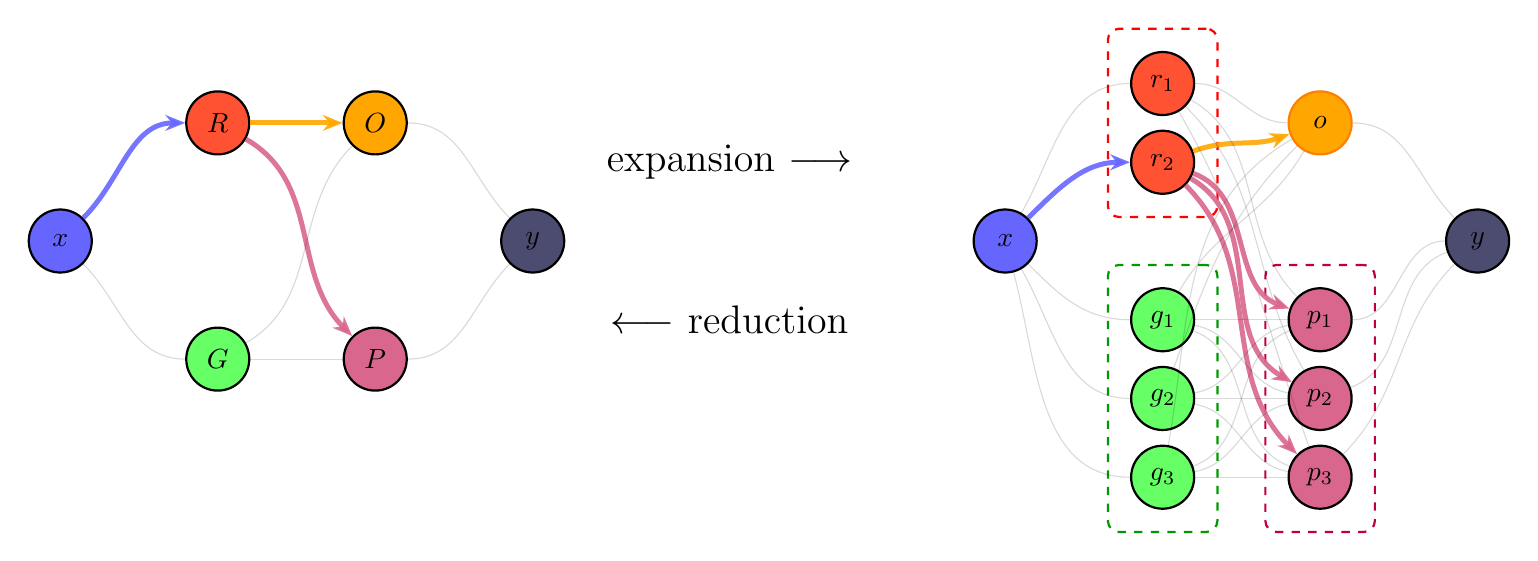
\begin{tikzpicture}[
    node/.style={circle, draw, minimum size=0.8cm, thick},
    xnode/.style={node, fill=blue!60},
    ynode/.style={node, fill=blue!20!black!70},
    rnode/.style={node, fill=red!70!orange!80},
    gnode/.style={node, fill=green!60},
    onode/.style={node, fill=orange!70!yellow},
    pnode/.style={node, fill=purple!60},
    % Edge styles
    faintedge/.style={black, opacity=0.15, thin},
    redge/.style={red!70!orange!80, opacity=0.9, line width=1.8pt, -{Stealth[length=2.5mm, width=2mm]}},
    gedge/.style={green!60, opacity=0.9, line width=1.8pt, -{Stealth[length=2.5mm, width=2mm]}},
    oedge/.style={orange!70!yellow, opacity=0.9, line width=1.8pt, -{Stealth[length=2.5mm, width=2mm]}},
    pedge/.style={purple!60, opacity=0.9, line width=1.8pt, -{Stealth[length=2.5mm, width=2mm]}},
    blueedge/.style={blue!60, opacity=0.9, line width=1.8pt, -{Stealth[length=2.5mm, width=2mm]}},
    arrow/.style={-{Latex[length=3mm]}, line width=3pt, gray!80},
    ]
    
    % Left network (simplified) with updated labels
    \node[xnode] (x1) at (0,0) {$x$};
    \node[rnode] (hr1) at (2,1.5) {$R$};
    \node[gnode] (hg1) at (2,-1.5) {$G$};
    \node[onode] (ho1) at (4,1.5) {$O$};
    \node[pnode] (hp1) at (4,-1.5) {$P$};
    \node[ynode] (y1) at (6,0) {$y$};
    
    % Connections for left network - all faint except those to/from hr1
    % x to hr1 (highlighted with arrow)
    \draw[blueedge] (x1) to[out=45, in=180] (hr1);
    % x to hg1 (faint)
    \draw[faintedge] (x1) to[out=-45, in=180] (hg1);
    % hr1 to ho1 (highlighted with arrow)
    \draw[oedge] (hr1) to[out=0, in=180] (ho1);
    % hr1 to hp1 (highlighted with arrow)
    \draw[pedge] (hr1) to[out=-30, in=135] (hp1);
    % hg1 to ho1 (faint)
    \draw[faintedge] (hg1) to[out=30, in=-135] (ho1);
    % hg1 to hp1 (faint)
    \draw[faintedge] (hg1) to[out=0, in=180] (hp1);
    % ho1 to y1 (faint)
    \draw[faintedge] (ho1) to[out=0, in=135] (y1);
    % hp1 to y1 (faint)
    \draw[faintedge] (hp1) to[out=0, in=-135] (y1);
    
    % Right network (expanded) - shifted horizontally with updated labels
    \node[xnode] (x2) at (12,0) {$x$};
    
    % Create multiple nodes for each color in the expanded network
    \node[rnode] (hr2_1) at (14,2) {$r_1$};
    \node[rnode] (hr2_2) at (14,1) {$r_2$};
    
    \node[gnode] (hg2_1) at (14,-1) {$g_1$};
    \node[gnode] (hg2_2) at (14,-2) {$g_2$};
    \node[gnode] (hg2_3) at (14,-3) {$g_3$};
    
    \node[onode, draw=orange, thick] (ho2) at (16,1.5) {$o$};
    
    \node[pnode] (hp2_1) at (16,-1) {$p_1$};
    \node[pnode] (hp2_2) at (16,-2) {$p_2$};
    \node[pnode] (hp2_3) at (16,-3) {$p_3$};
    
    \node[ynode] (y2) at (18,0) {$y$};
    
    % Connections from x to all red and green nodes
    \draw[faintedge] (x2) to[out=60, in=180] (hr2_1);
    \draw[blueedge] (x2) to[out=45, in=180] (hr2_2); % Highlighted with arrow
    \draw[faintedge] (x2) to[out=-45, in=180] (hg2_1);
    \draw[faintedge] (x2) to[out=-60, in=180] (hg2_2);
    \draw[faintedge] (x2) to[out=-75, in=180] (hg2_3);
    
    % Connections from all red nodes to orange node
    \draw[faintedge] (hr2_1) to[out=0, in=180] (ho2);
    \draw[oedge] (hr2_2) to[out=20, in=200] (ho2); % Highlighted with arrow
    
    % Connections from all red nodes to all purple nodes
    \draw[faintedge] (hr2_1) to[out=-30, in=135] (hp2_1);
    \draw[faintedge] (hr2_1) to[out=-45, in=120] (hp2_2);
    \draw[faintedge] (hr2_1) to[out=-60, in=110] (hp2_3);
    
    \draw[pedge] (hr2_2) to[out=-20, in=160] (hp2_1); % Highlighted with arrow
    \draw[pedge] (hr2_2) to[out=-30, in=150] (hp2_2); % Highlighted with arrow
    \draw[pedge] (hr2_2) to[out=-45, in=135] (hp2_3); % Highlighted with arrow
    
    % Connections from all green nodes to orange node
    \draw[faintedge] (hg2_1) to[out=60, in=-120] (ho2);
    \draw[faintedge] (hg2_2) to[out=70, in=-135] (ho2);
    \draw[faintedge] (hg2_3) to[out=80, in=-150] (ho2);
    
    % Connections from all green nodes to all purple nodes
    % All faint as they don't connect to hr2_2
    \draw[faintedge] (hg2_1) to[out=0, in=180] (hp2_1);
    \draw[faintedge] (hg2_1) to[out=-10, in=170] (hp2_2);
    \draw[faintedge] (hg2_1) to[out=-20, in=160] (hp2_3);
    
    \draw[faintedge] (hg2_2) to[out=10, in=190] (hp2_1);
    \draw[faintedge] (hg2_2) to[out=0, in=180] (hp2_2);
    \draw[faintedge] (hg2_2) to[out=-10, in=170] (hp2_3);
    
    \draw[faintedge] (hg2_3) to[out=20, in=200] (hp2_1);
    \draw[faintedge] (hg2_3) to[out=10, in=190] (hp2_2);
    \draw[faintedge] (hg2_3) to[out=0, in=180] (hp2_3);
    
    % Connections from orange to y (faint since not directly from hr2_2)
    \draw[faintedge] (ho2) to[out=0, in=135] (y2);
    
    % Connections from all purple nodes to y (faint since not directly from hr2_2)
    \draw[faintedge] (hp2_1) to[out=0, in=180] (y2);
    \draw[faintedge] (hp2_2) to[out=20, in=-160] (y2);
    \draw[faintedge] (hp2_3) to[out=45, in=-135] (y2);
    
    % Add dashed outlines around groups
    \begin{pgfonlayer}{background}
        \node[draw=red, dashed, thick, rounded corners, fit=(hr2_1) (hr2_2), inner sep=8pt] {};
        \node[draw=green!60!black, dashed, thick, rounded corners, fit=(hg2_1) (hg2_2) (hg2_3), inner sep=8pt] {};
        \node[draw=purple, dashed, thick, rounded corners, fit=(hp2_1) (hp2_2) (hp2_3), inner sep=8pt] {};
    \end{pgfonlayer}
    
    % Add horizontal arrows for reduction and expansion
    \node at (8.5,1) {\Large expansion $\longrightarrow$};
    \node at (8.5,-1) {\Large $\longleftarrow$ reduction};
    
\end{tikzpicture}
}
    \caption{Illustration of network expansion and reduction according to Proposition~\ref{prop:cloned}. A cloned network $\widetilde{G}$ (left) with node partitions $\{S_v\}$ can, under specific weight initializations, behave identically to a narrower network $G$ (right). Gradient descent confines the parameters of $\widetilde{G}$ to a low-dimensional manifold isomorphic to the parameter space of $G$, inducing structural loss of plasticity.}
    \label{fig:plasticity-manifolds}
\end{figure}

\begin{remark}
The affine subspace identified in Proposition~\ref{prop:cloned} acts as a stable manifold for any optimizer relying solely on first-order gradient information (like SGD, Momentum, Adam) because the gradients themselves respect the cloning symmetry. This holds regardless of the data distribution encountered.
\end{remark}
\giulia{This remarked should be emphasised!}

\giulia{I would place the results of the experiments showing the emergence of LoP symptoms here, as it should make a more convincing argument for the reader, and make it less abstract.}

\begin{figure}[h!]
    \centering
    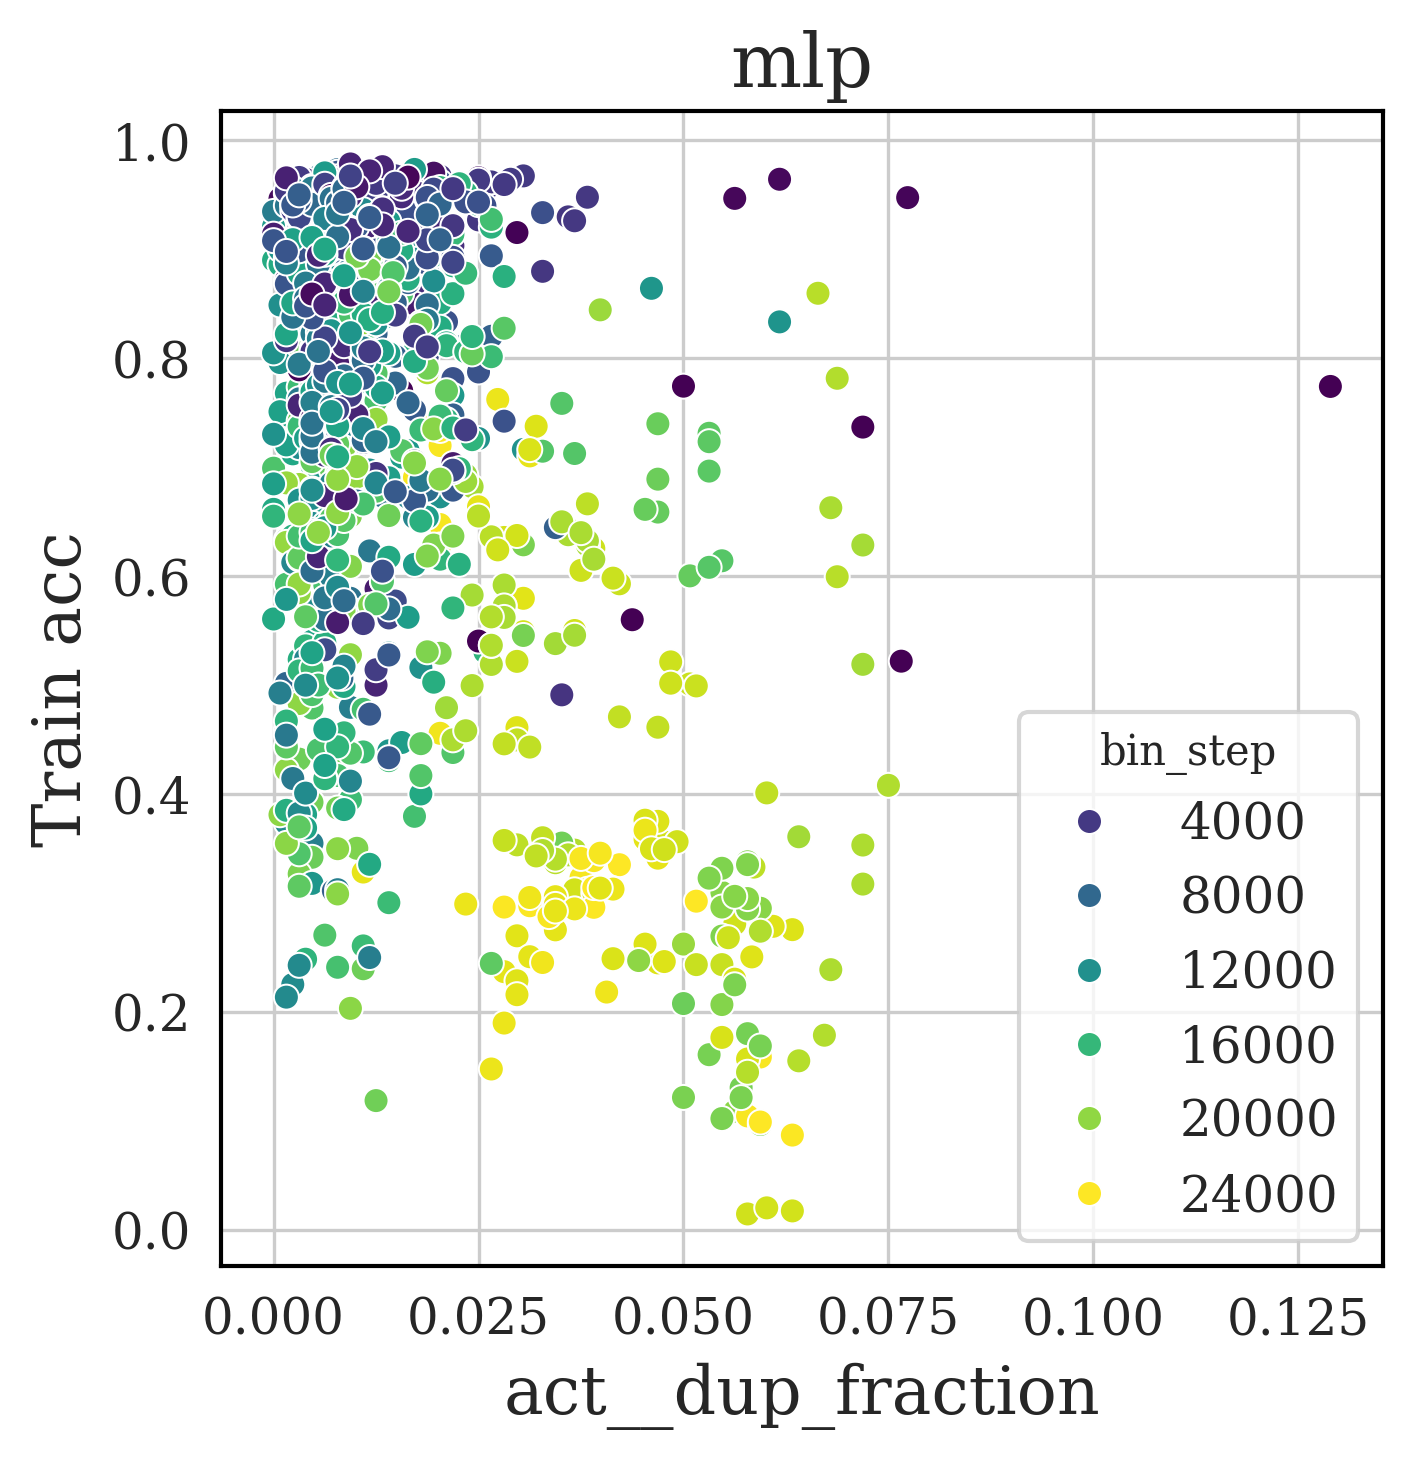
\includegraphics[width=0.24\linewidth]{paper/images/mlp_dup_frac.png}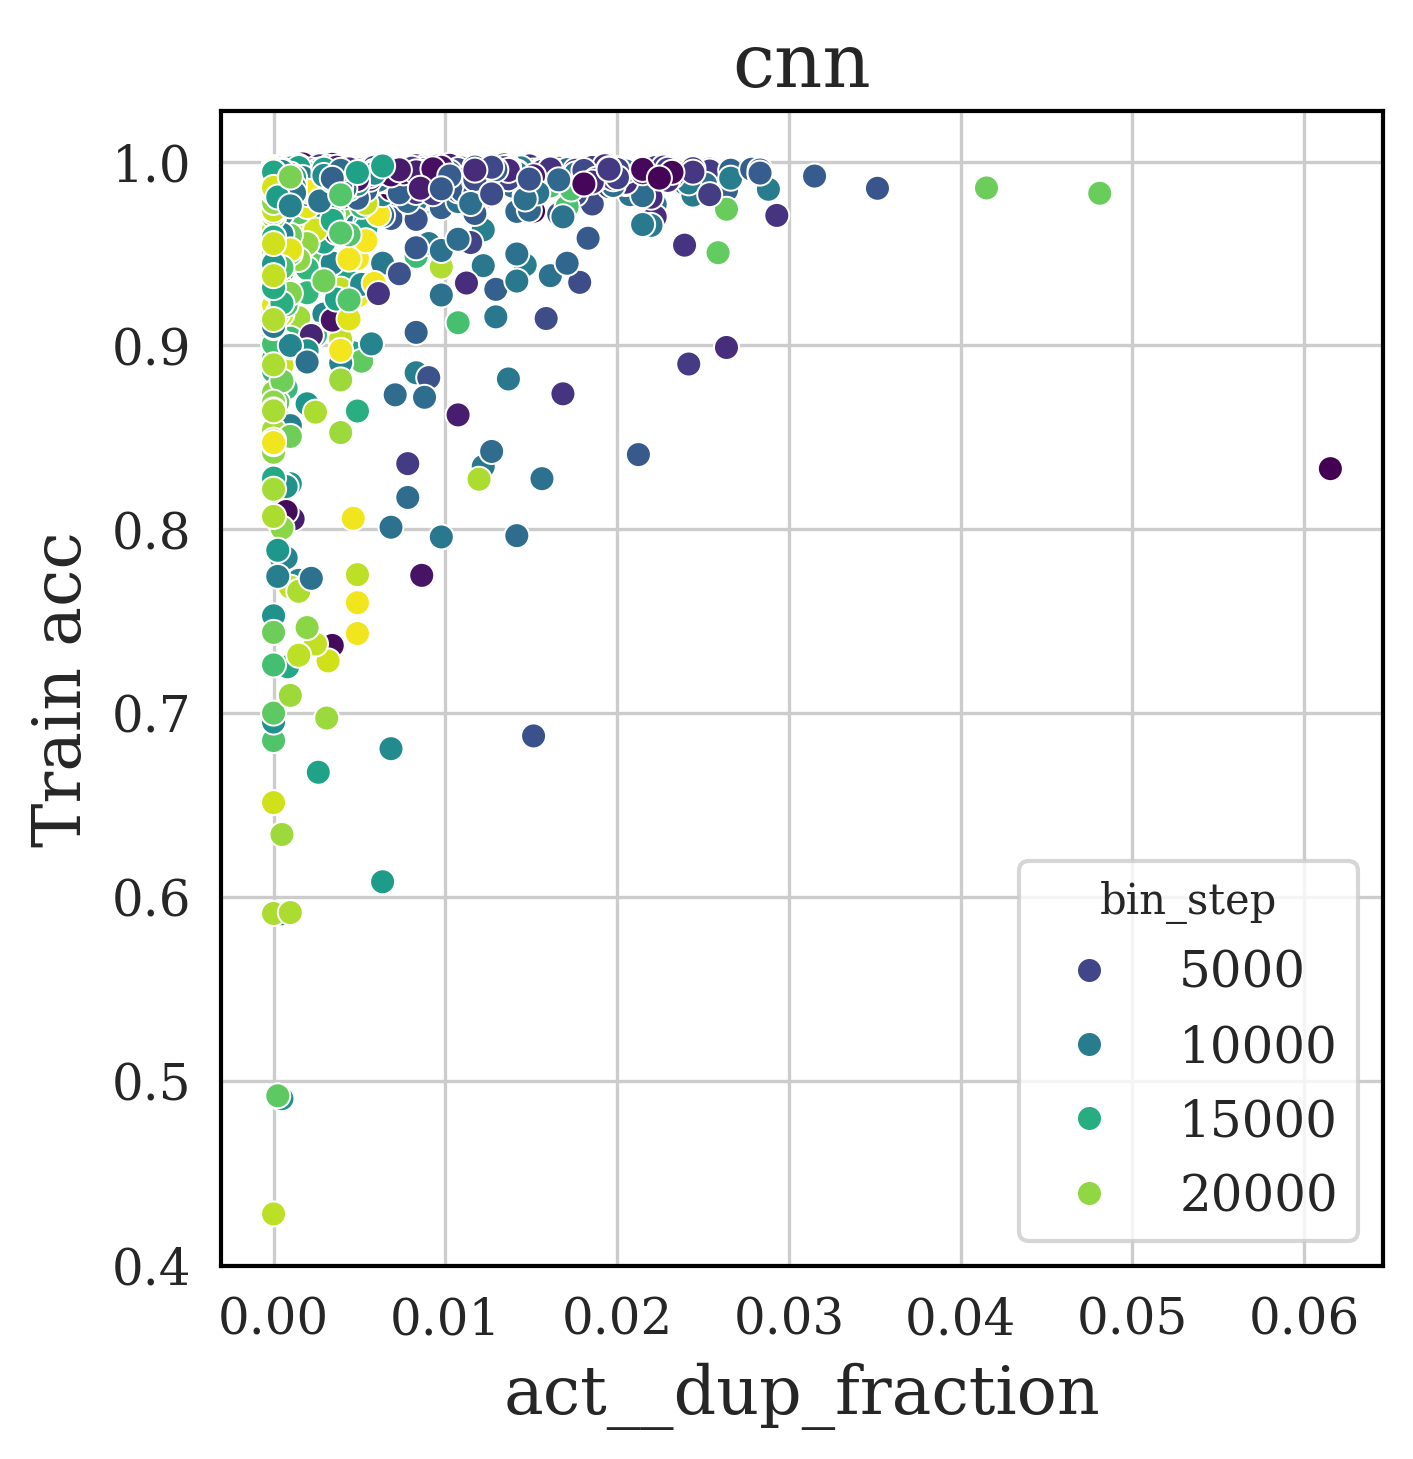
\includegraphics[width=0.24\linewidth]{paper/images/cnn_dup_frac.png}
    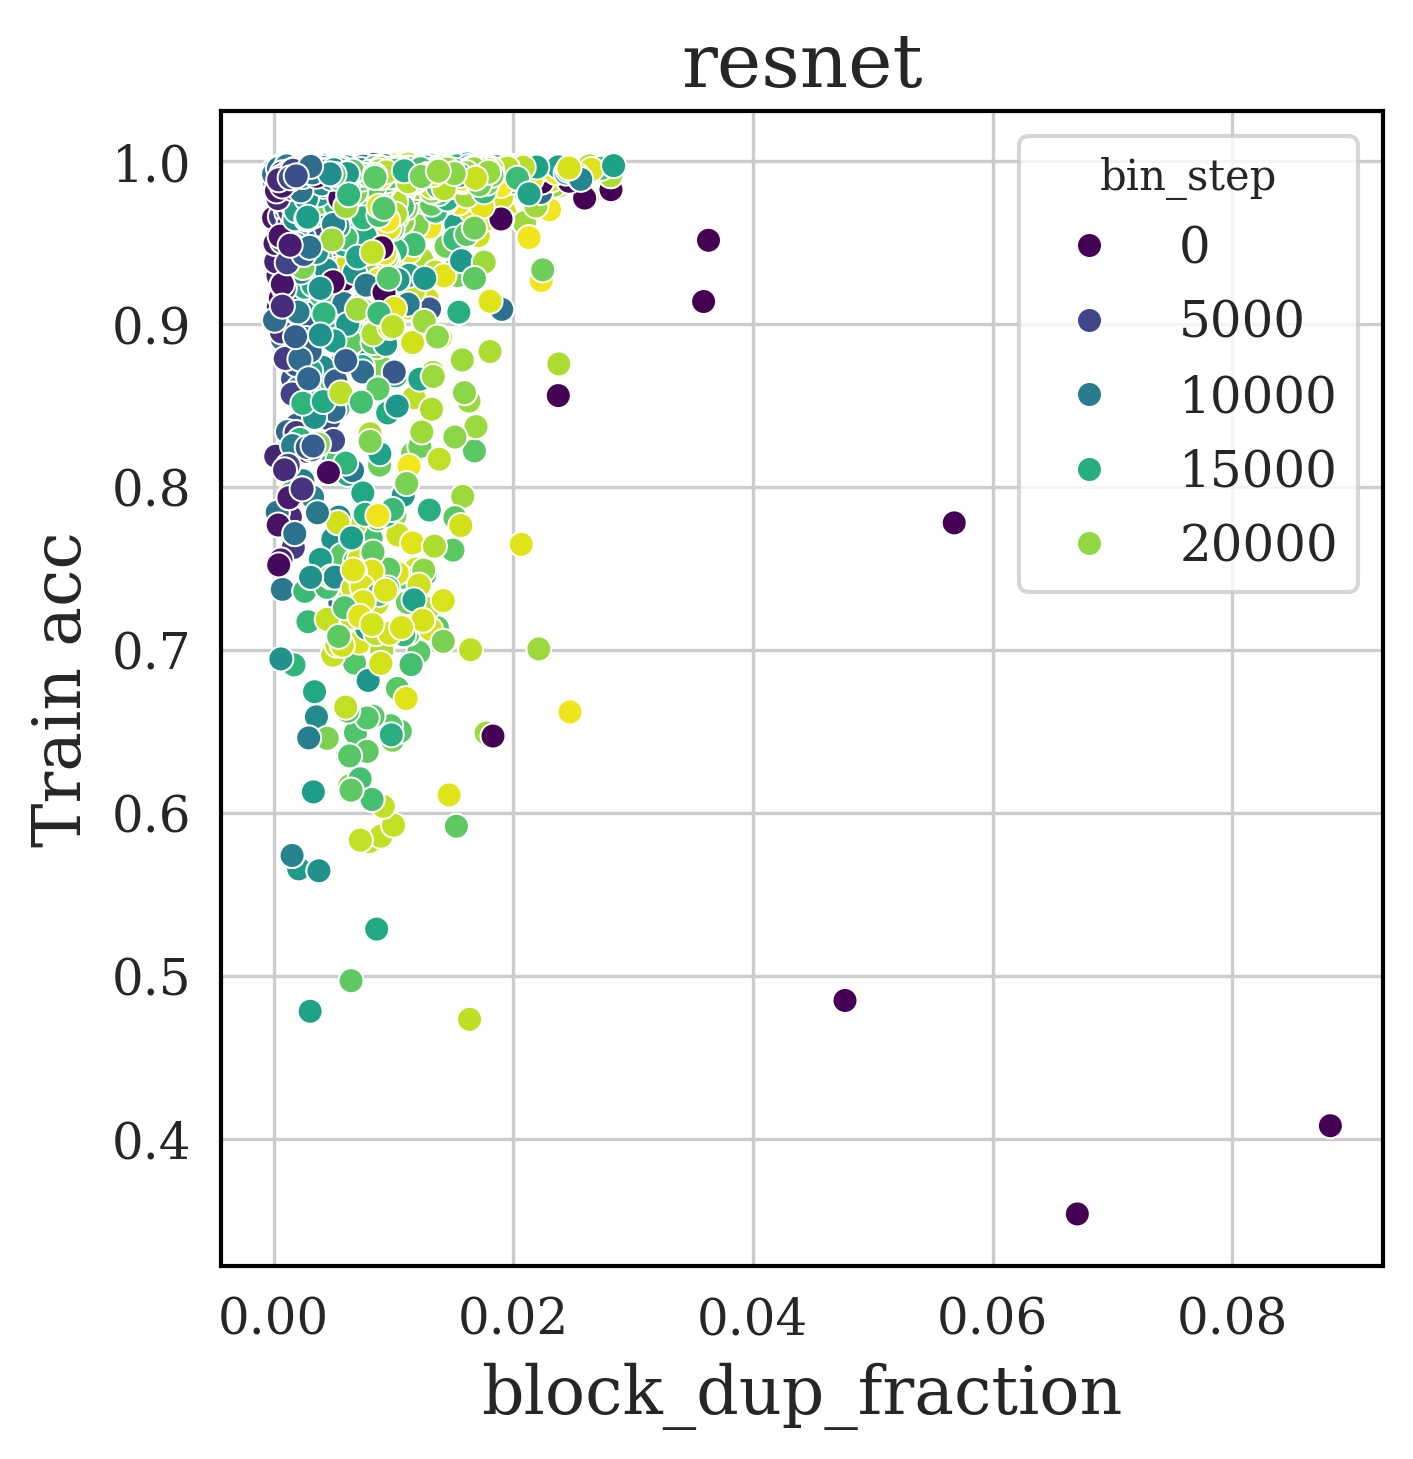
\includegraphics[width=0.24\linewidth]{paper/images/resnet_dup_frac.png}
    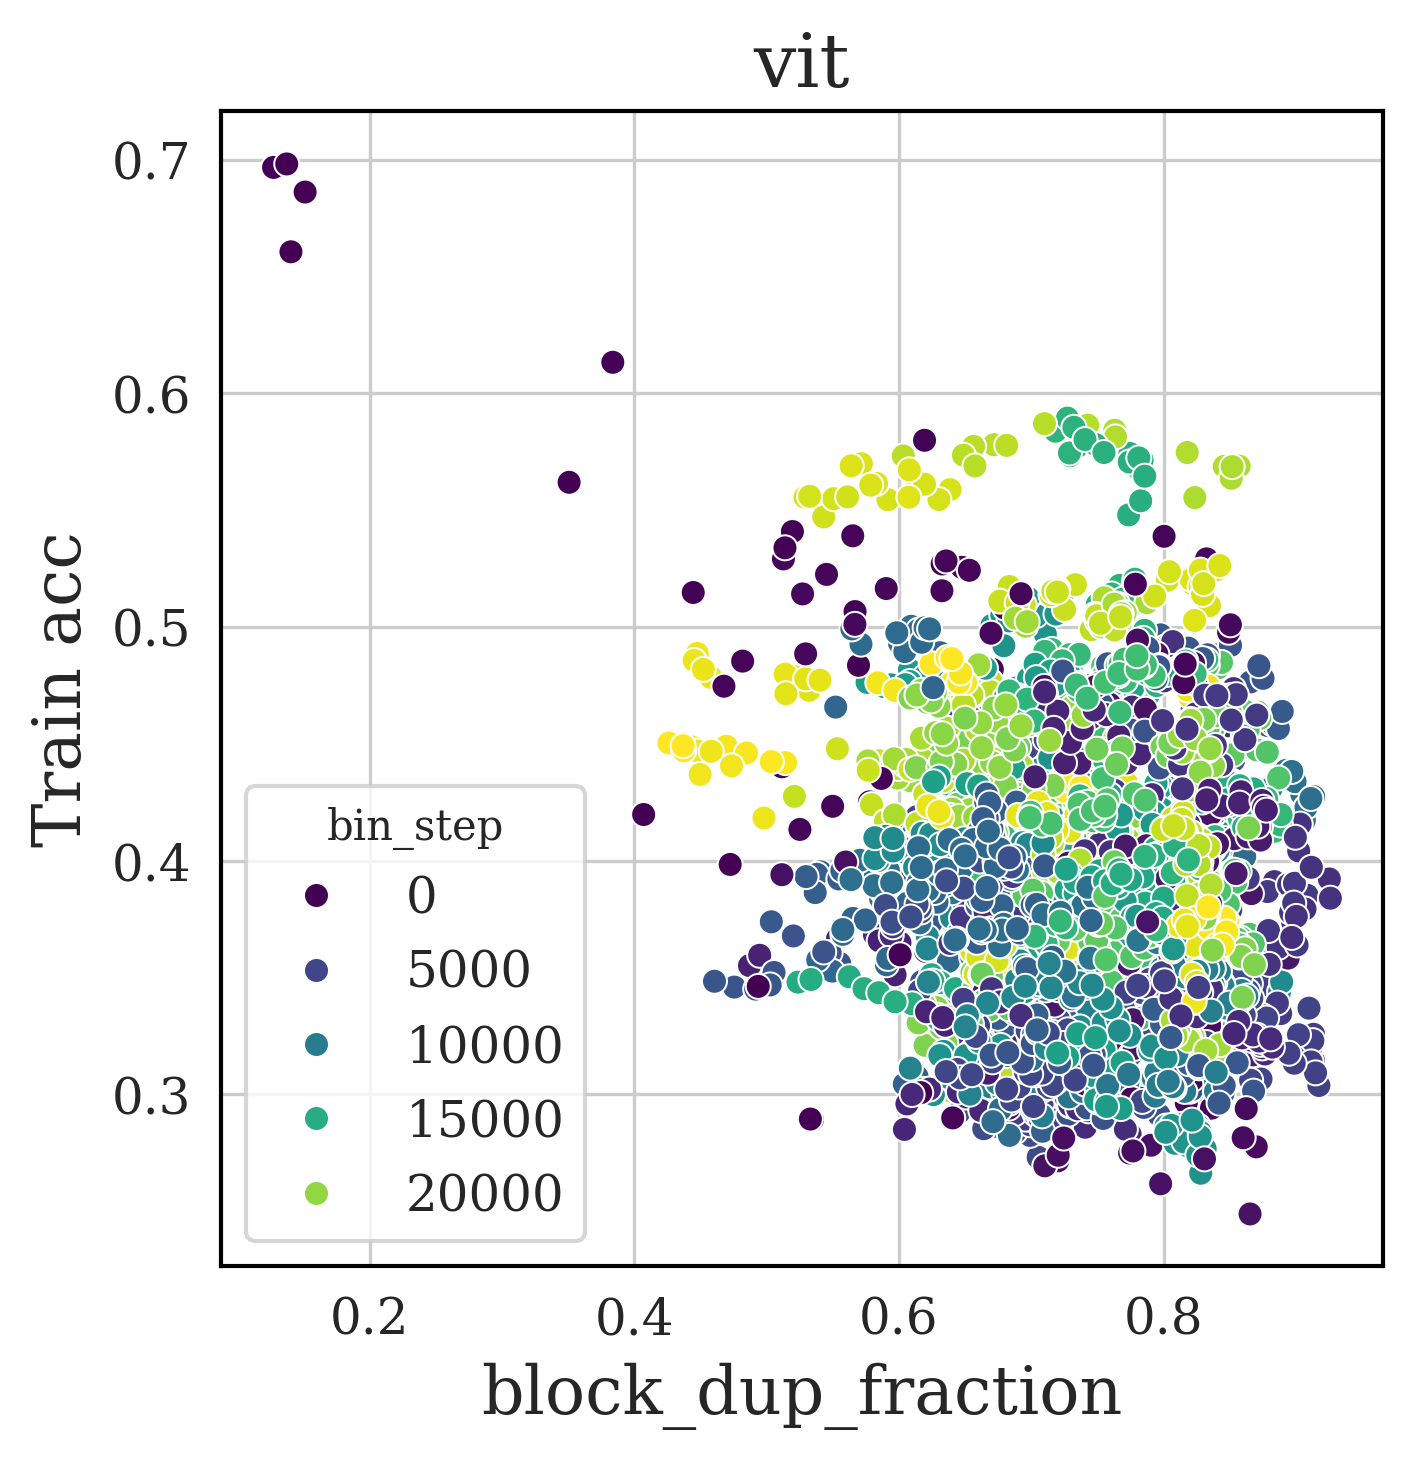
\includegraphics[width=0.24\linewidth]{paper/images/vit_dup_frac.png}
    \caption{(Placeholder figure, not final) No normalization (except layer for vit) and no dropout. The colours correspond to training steps (binned for convenienc). This figure shows the emergence of duplicate units during training, and their relation with the training performance.}
    \label{fig:dupfrac-LoP}
\end{figure}
\begin{figure}[h!]
    \centering
    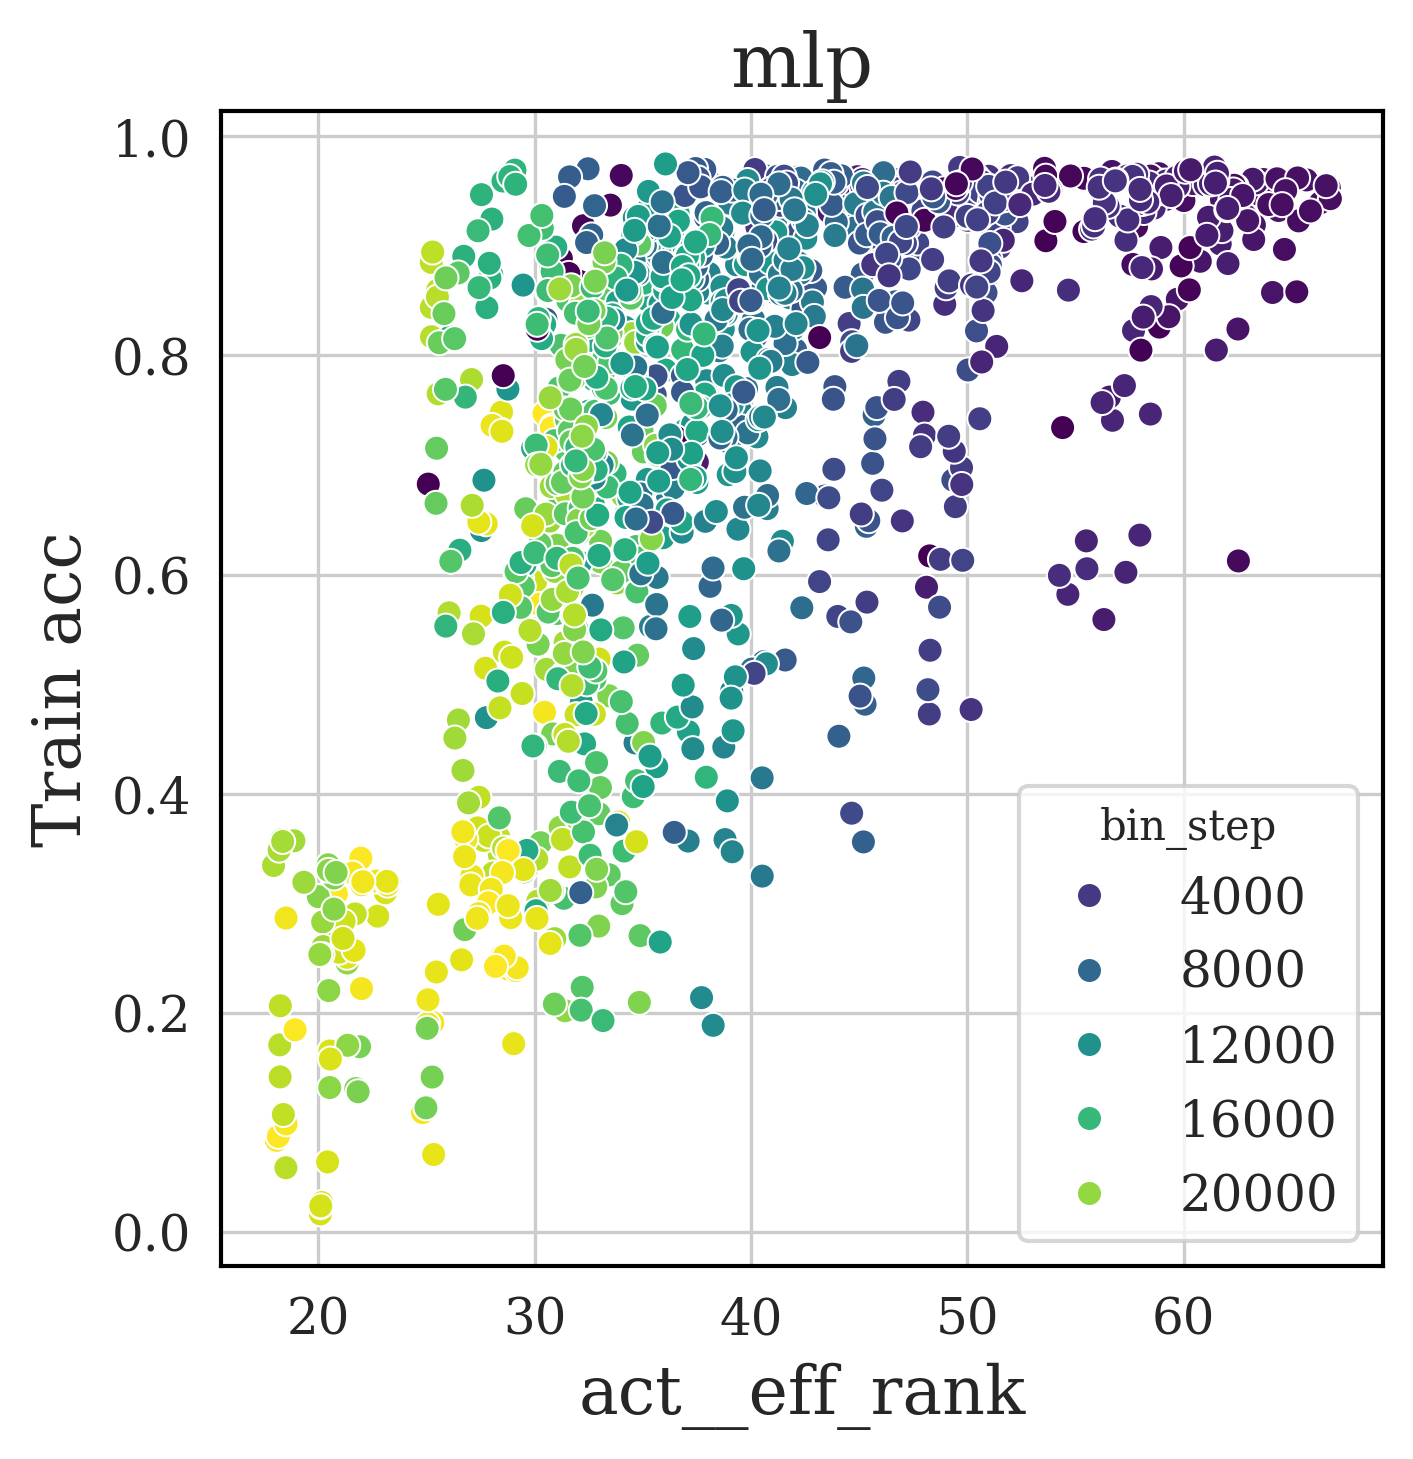
\includegraphics[width=0.24\linewidth]{paper/images/mlp_stable_rank.png}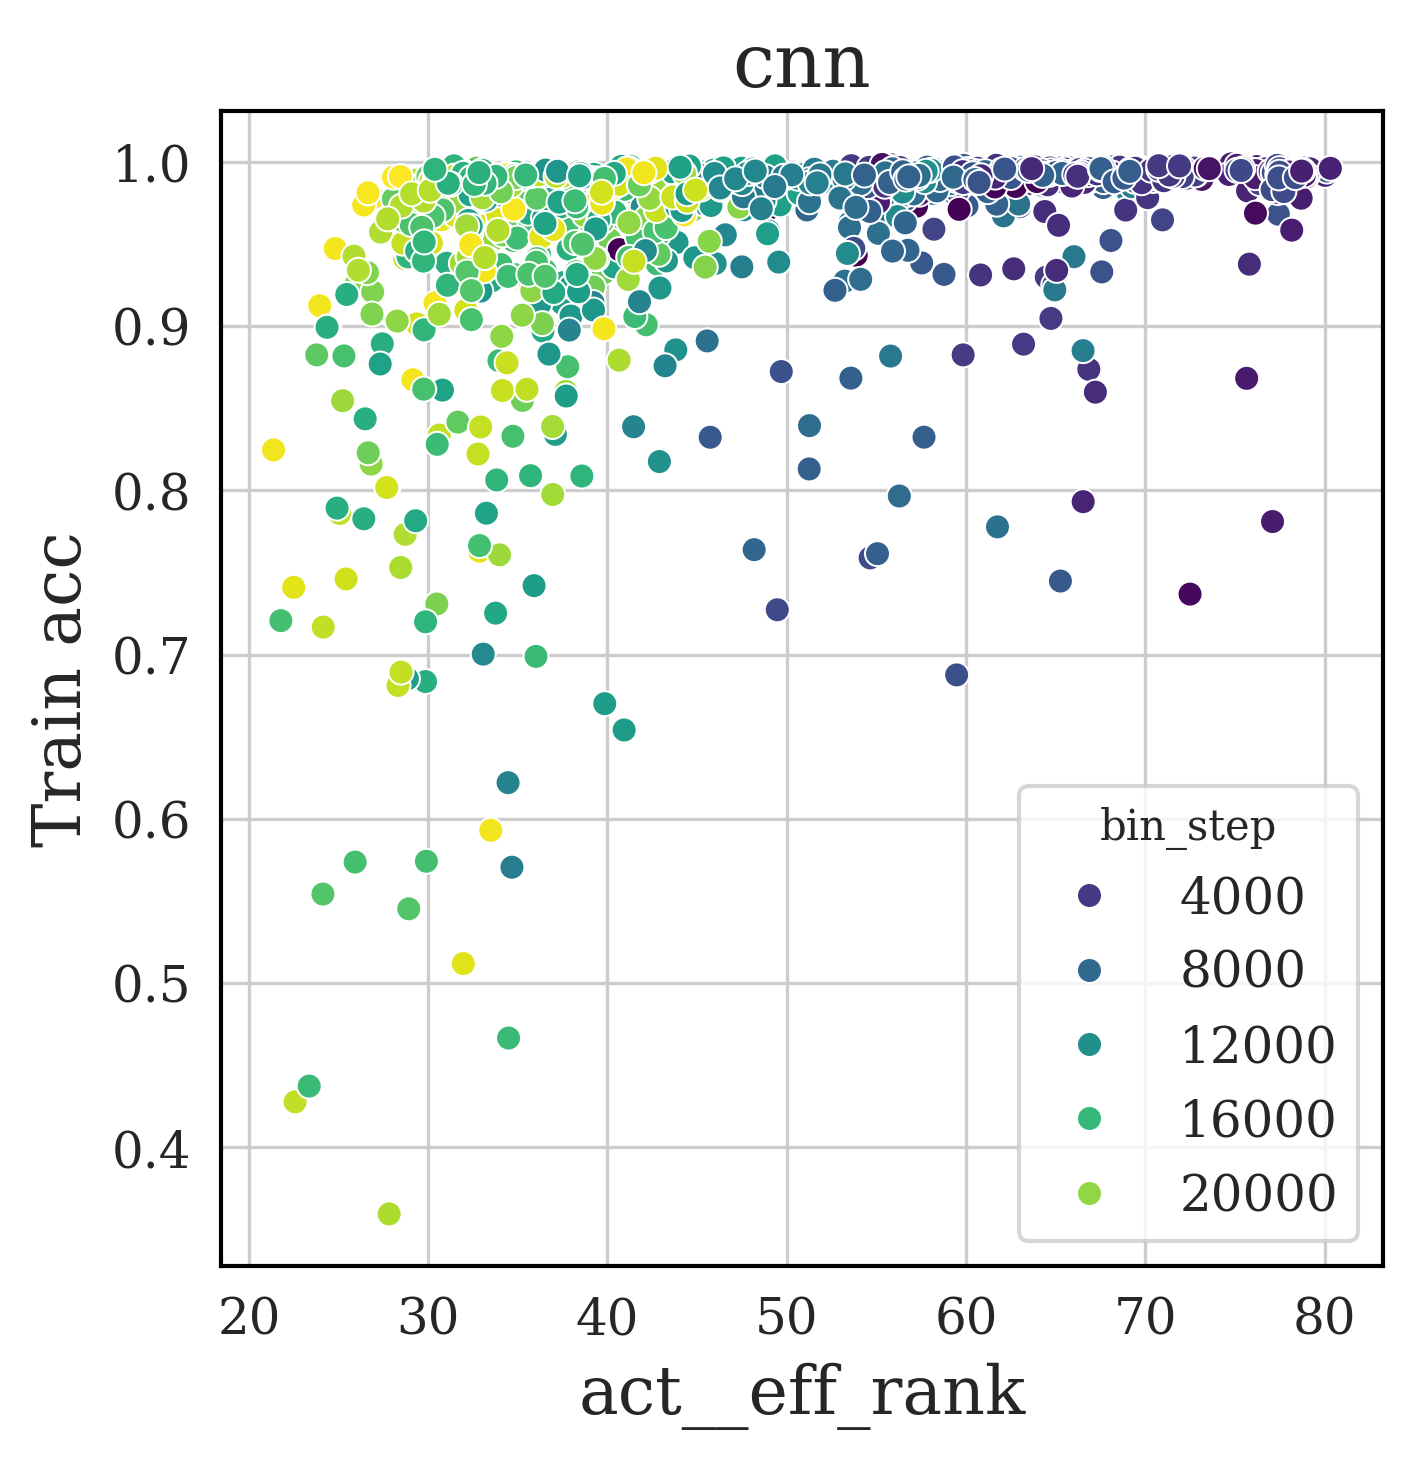
\includegraphics[width=0.24\linewidth]{paper/images/cnn_stable_rank.png}
    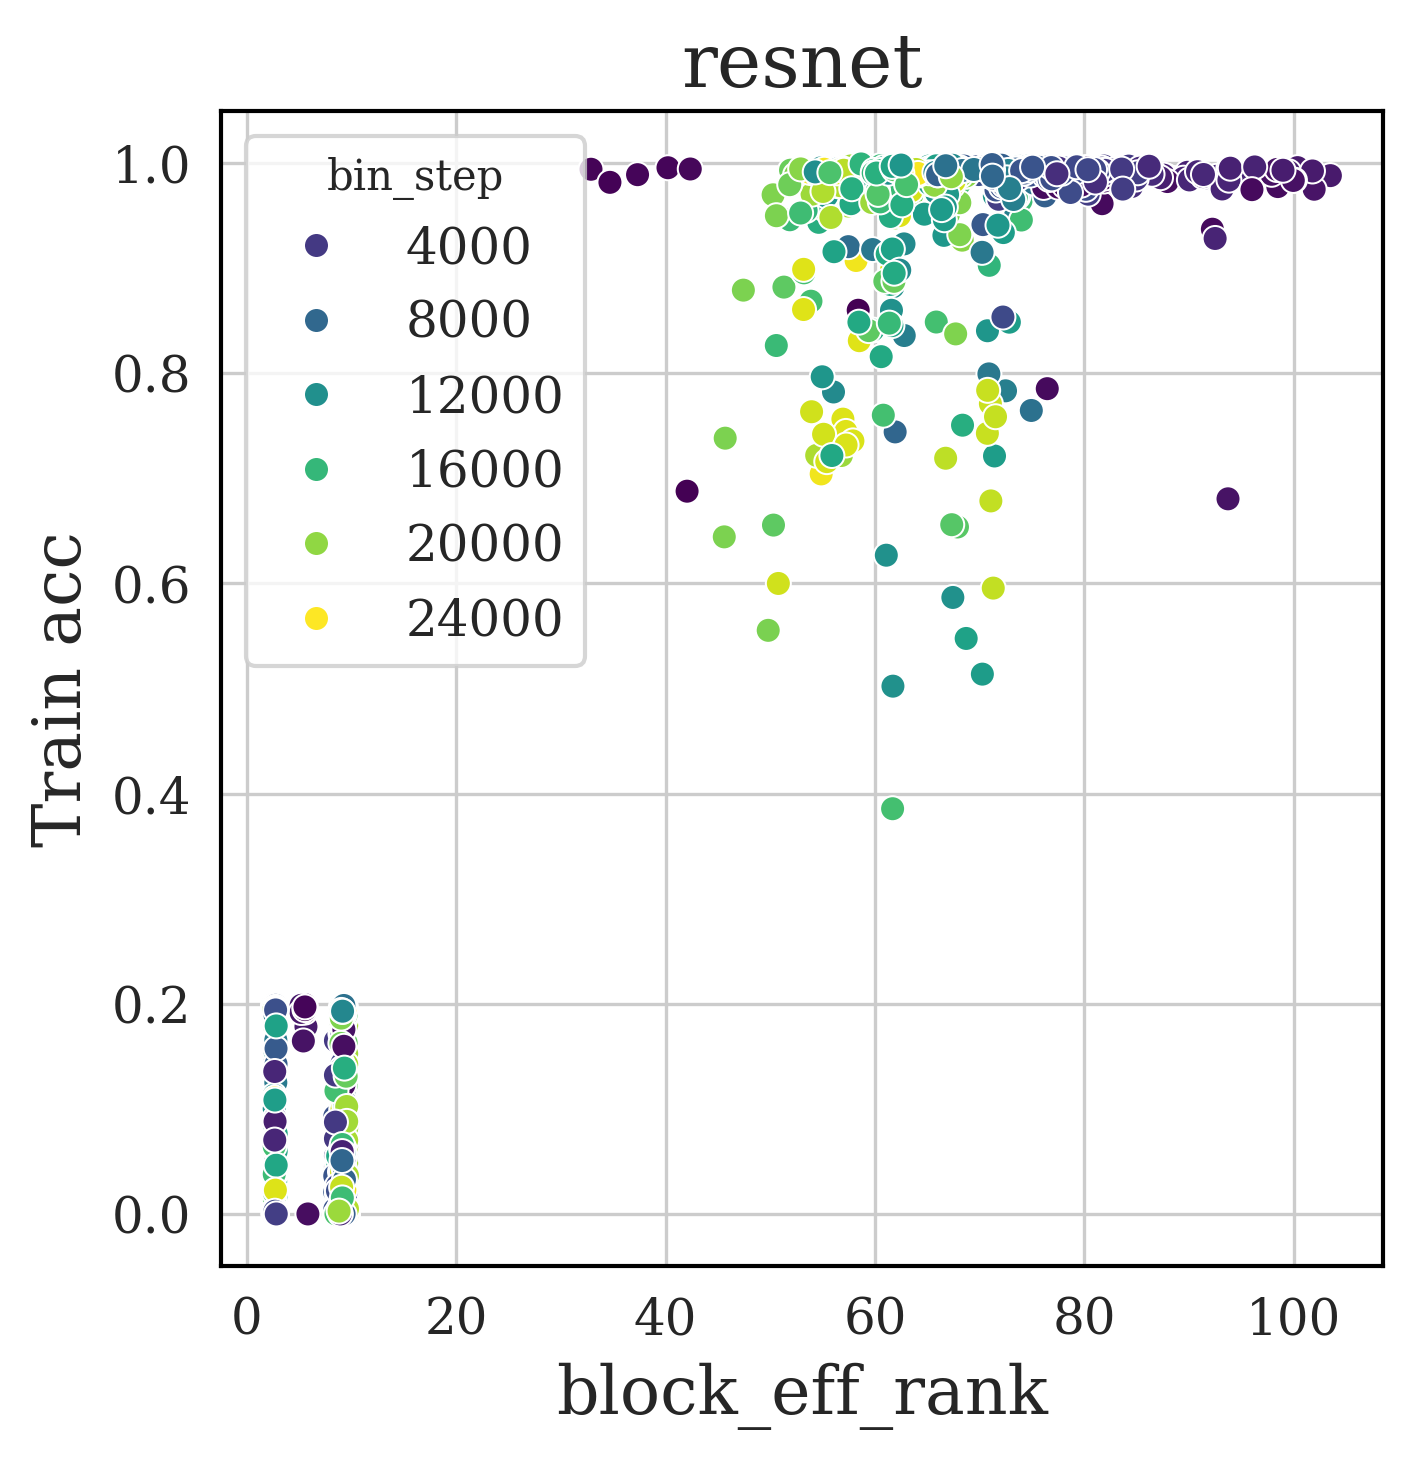
\includegraphics[width=0.24\linewidth]{paper/images/resnet_stable_rank.png}
    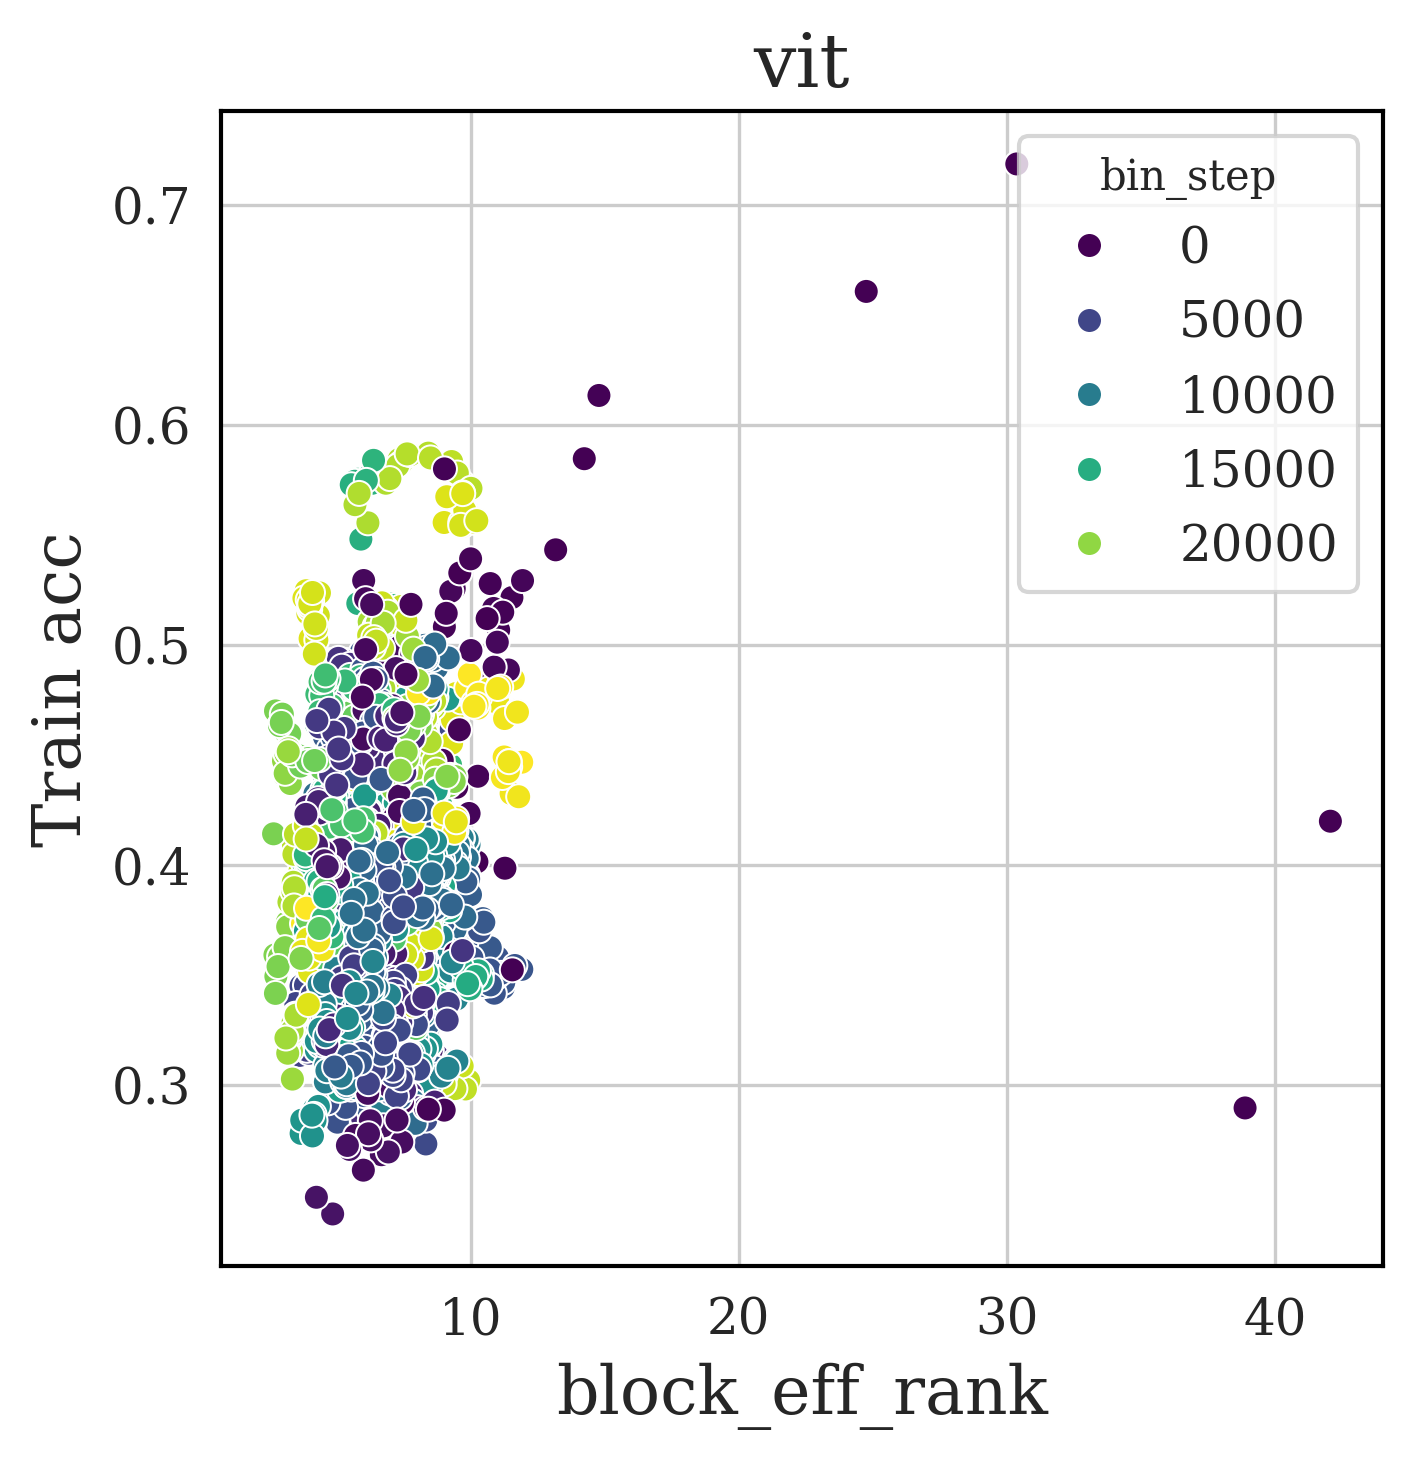
\includegraphics[width=0.24\linewidth]{paper/images/vit_stable_rank.png}
    \caption{(Placeholder figure, not final) No normalization (except layer for vit) and no dropout. The colours correspond to training steps (binned for convenienc). This figure shows the evolution of the features stable rank during training, and their relation with the training performance.}
    \label{fig:dupfrac-LoP}
\end{figure}
\section{Mitigating and Recovering Plasticity}
\label{sec:mitigate}

Having identified mechanisms leading to plasticity loss, we now consider strategies suggested by the theory to prevent or escape these traps.

\giulia{Personal opinion: I think this section should be restructured. In particular, I would start with dropout and continual backprop, which both inject noise during the optimization process, with the result of de-correlating features. Then I would discuss separately the less obvious case of Gaussian features, and show that Batch Normalization indeed achieves this to some extent.}

\subsection{Rank recovery via nonlinear activations}

One way plasticity is lost is through the collapse of representational diversity, manifesting as low-rank feature spaces (as potentially induced by cloned units or other dynamics). Maintaining higher-rank representations could thus preserve plasticity. Certain architectural choices and properties of activation functions can promote this.

\begin{proposition}
\label{prop:rank}
Let $f:\R\to\R$ be non-linear activation that is not a bounded degree polynomial and is square-integrable with respect to the Gaussian kernel $\mathcal{N}(0,1)$. Consider a vector of pre-activations $z\in\R^d$ whose components are jointly Gaussian, $z \sim \mathcal{N}(0, \Sigma)$, with covariance matrix $\Sigma$ such that $\E[z_i z_j]=\Sigma_{ij}$ and $|\Sigma_{ij}|<1$ for $i \neq j$ (assuming unit variance for simplicity, $\Sigma_{ii}=1$). Then the covariance matrix of the post-activations $C = \E[f(z)f(z)^\top]$ is full rank, unless some features are perfectly correlated or anti-correlated (i.e., $|\Sigma_{ij}|=1$) or are exact duplicates.
\end{proposition}

The proof (Appendix~\ref{app:proofs}) leverages the Hermite polynomial expansion of the activation function $f$ \cite{erdelyi1953higher} and Mehler's formula for the expectation of products of Hermite polynomials of correlated Gaussian variables \cite{mehler1866ueber, erdelyi1953higher}. Since a non-polynomial function has infinitely many non-zero Hermite coefficients, the resulting covariance matrix becomes a sum of positive semidefinite matrices (Hadamard powers of $\Sigma$), which generally results in a positive definite (full rank) matrix unless the underlying Gaussian variables $z_i$ lack diversity.

% Assuming this follows the discussion of Proposition 3.3 (labeled prop:rank)
% within \subsection{Rank Preservation via Nonlinearities and Gaussianity}

While Proposition~\ref{prop:rank} highlights that non-linear activations are key to rank recovery from rank-deficient pre-activations (assuming Gaussian inputs), their \emph{effective nonlinearity} in practice hinges on the input statistics (e.g., mean, variance, range). If pre-activations fall into linear or saturated regimes (e.g., Tanh for small inputs, ReLU for all-positive inputs), the activation's ability to expand rank diminishes, as it behaves like an affine transformation. The following simulations illustrate this dependency and how controlling input statistics, e.g., via normalization, ensures activations operate in beneficial non-linear regimes. We use synthetic low-rank pre-activations $z \in \R^{d}$, having $d_{\text{full}}=20$ dimensions with a hard rank of $5$, and show that Tanh activation is able to improve the conditioning of post-activation eigenvalues, and thereby effective rank of post-activations. In case of ReLU activation, you can see in Figure~\ref{fig:theory_relu_zb_rank}, that if we shift the pre-activations to become all-positive, ReLU behaves like an affine transform and is not able to improve the conditioning. These observations point to the interplay between normalizaion and activations, in that, normalization layers ensure that activations remain effectively non-linear, thereby can improve rank of pre-activations. 

\begin{figure}[ht!]
    \centering
    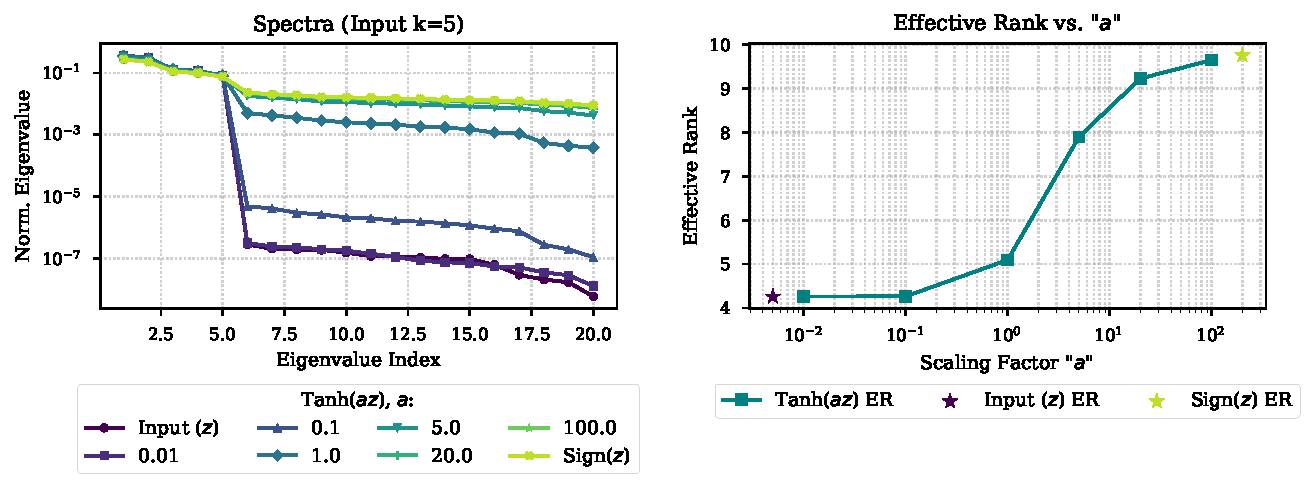
\includegraphics[width=0.7\linewidth]{figures/theory_tanh_az_rank.pdf} % Assuming image is in figures/
    \caption{Effect of input scaling on post-activation effective rank for $h = \tanh(az)$, with rank-deficient $z$ (initial ER=5, $d_{\text{full}}=20$). \textbf{Left:} Normalized eigenvalue spectra of $\mathrm{Cov}(h)$. \textbf{Right:} Effective rank of $\mathrm{Cov}(h)$ vs. scaling $a$. Small $a$ leads to linear behavior ($\tanh(az) \approx az$) and minimal rank increase. Appropriate $a$ enhances non-linearity and rank recovery. Very large $a$ makes $\tanh(az) \approx \mathrm{sign}(z)$, also yielding high rank.}
    \label{fig:theory_tanh_az_rank}
\end{figure}

% In Section 4.1, after discussion of Prop 4.1, Figure 5, and Appendix A synthetic figs:

These theoretical considerations and synthetic experiments (Figure~\ref{fig:theory_tanh_az_rank}, and Figures~\ref{fig:theory_relu_zb_rank}, \ref{fig:theory_joint_norm_activation_rank} in Appendix~\ref{app:rank_validation_appendix_label}) highlight the importance of maintaining pre-activations within the effective non-linear range of activation functions for rank recovery. 
To demonstrate this in a practical deep learning context, we empirically investigate the progression of effective rank in Multi-Layer Perceptrons (MLPs) trained on the MNIST dataset. Figure~\ref{fig:empirical_rank_progression} compares models utilizing ReLU activations with no normalization, Batch Normalization, and Layer Normalization across training epochs. Additional empirical results, including the evolution of other metrics like frozen and duplicate units, can be found in Appendix~\ref{app:additional_empirical_evidence}.

To complement the rank progression analysis in Section~\ref{sec:mitigate} (specifically Figure~\ref{fig:empirical_rank_progression}), Figure~\ref{fig:empirical_all_metrics} provides a broader view of network health metrics for the MLP model trained on MNIST with ReLU activation. This includes the effective rank, percentage of frozen units (pre-activations consistently in the zero-gradient regime of ReLU), and percentage of duplicate units (highly correlated neurons) at selected epochs.


\begin{figure}[ht!]
    \centering
    % Ensure this figure path and name are correct, e.g., figures/empirical_rank_progression_relu_mnist.pdf
    % Adjust width as needed; \textwidth might be suitable for a preprint single-column format.
    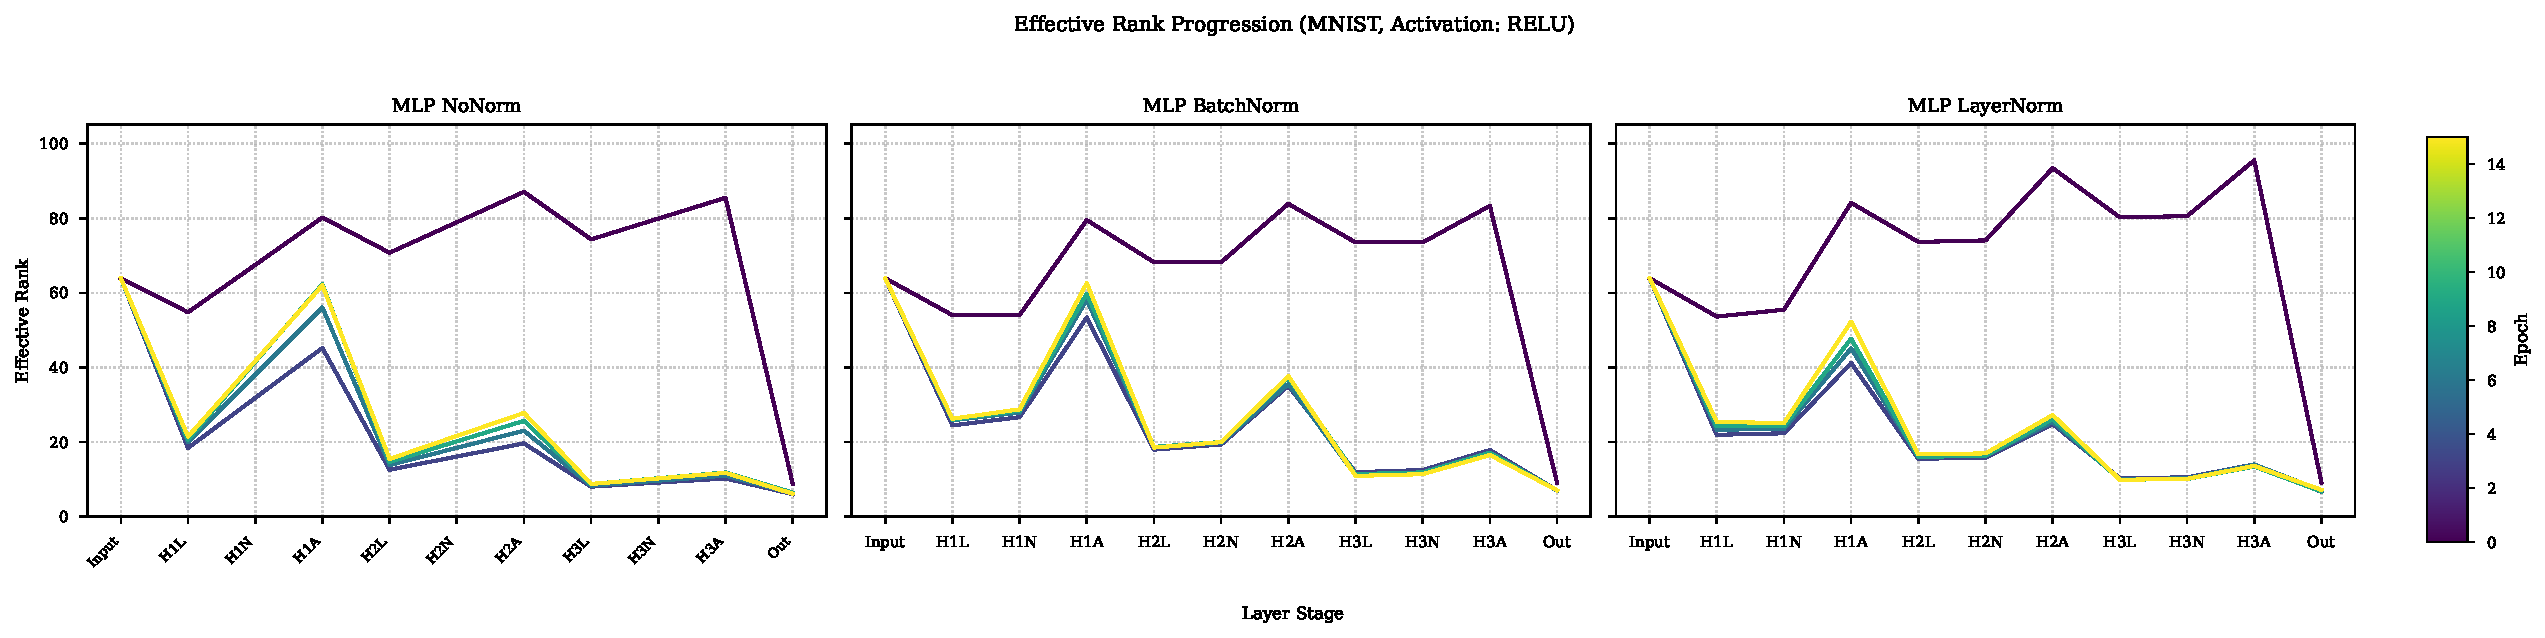
\includegraphics[width=\textwidth]{figures/empirical_rank_progression_relu_mnist.pdf} 
    \caption{Empirical effective rank progression in an MLP trained on MNIST with ReLU activations. Subplots compare models with no normalization (left panel), Batch Normalization (center panel), and Layer Normalization (right panel). Lines within each subplot show the effective rank across network layers at different epochs (indicated by the color bar, typically progressing from early (e.g., dark blue/purple) to later (e.g., yellow/light green) epochs).}
    \label{fig:empirical_rank_progression}
\end{figure}

Figure~\ref{fig:empirical_rank_progression} illustrates that non-linear activations inherently contribute to maintaining feature diversity; even the model without normalization (left panel) shows non-trivial effective rank across layers, a testament to the rank-expanding capability of the ReLU activation itself when inputs are not entirely collapsed or saturated. However, this model can experience a more pronounced decrease in effective rank in deeper layers or as training progresses compared to its normalized counterparts. Both Batch Normalization (center panel) and Layer Normalization (right panel) generally sustain a higher effective rank across the network over more epochs. This empirical evidence supports the hypothesis that while non-linear activations are the primary drivers of rank recovery, normalization techniques significantly facilitate this process. They achieve this by conditioning the inputs to these activations, likely preventing them from operating in saturated or overly linear regimes where their rank-expanding capabilities are diminished.

% Then, transition to "Design implications."
% \paragraph{Design implications.}
% These findings underscore the role of specific design choices in promoting plasticity by preserving representational rank:
% \begin{itemize}
%     \item \textbf{Batch Normalization (BatchNorm):} % ... (current text can follow)
% % ...
% \end{itemize}


\giulia{Here we should discuss the Proposition and its implications. }

\paragraph{Design implications.}
This proposition provides theoretical grounding for the empirical success of certain techniques in maintaining network health and potentially plasticity:
\begin{itemize}
    \item \textbf{Batch Normalization (BatchNorm):} Proposed by \cite{ioffe2015batch}, BatchNorm normalizes layer inputs to have approximately zero mean and unit variance. By stabilizing and somewhat Gaussianizing the distribution of pre-activations, BatchNorm helps satisfy the conditions of Proposition~\ref{prop:rank}, thereby combating rank collapse and potentially delaying plasticity loss. It aims to reduce ``internal covariate shift'', which can contribute to saturation and instability.[10]
    \item \textbf{Dropout:} Introduced by \cite{srivastava2014dropout}, Dropout randomly sets a fraction of neuron activations to zero during training. This prevents complex co-adaptations and breaks symmetries in the network. By continually introducing stochasticity and preventing units from becoming overly reliant on each other, Dropout can disrupt the formation of cloned-unit manifolds (Proposition~\ref{prop:cloned}) and help maintain representational diversity, thus preserving rank and plasticity.
\end{itemize}
These techniques, while often motivated by improving optimization speed or static generalization, can be reinterpreted through our framework as mechanisms that counteract the dynamics leading to plasticity loss by preserving representational rank and diversity.

\begin{figure}[h!]
    \centering
    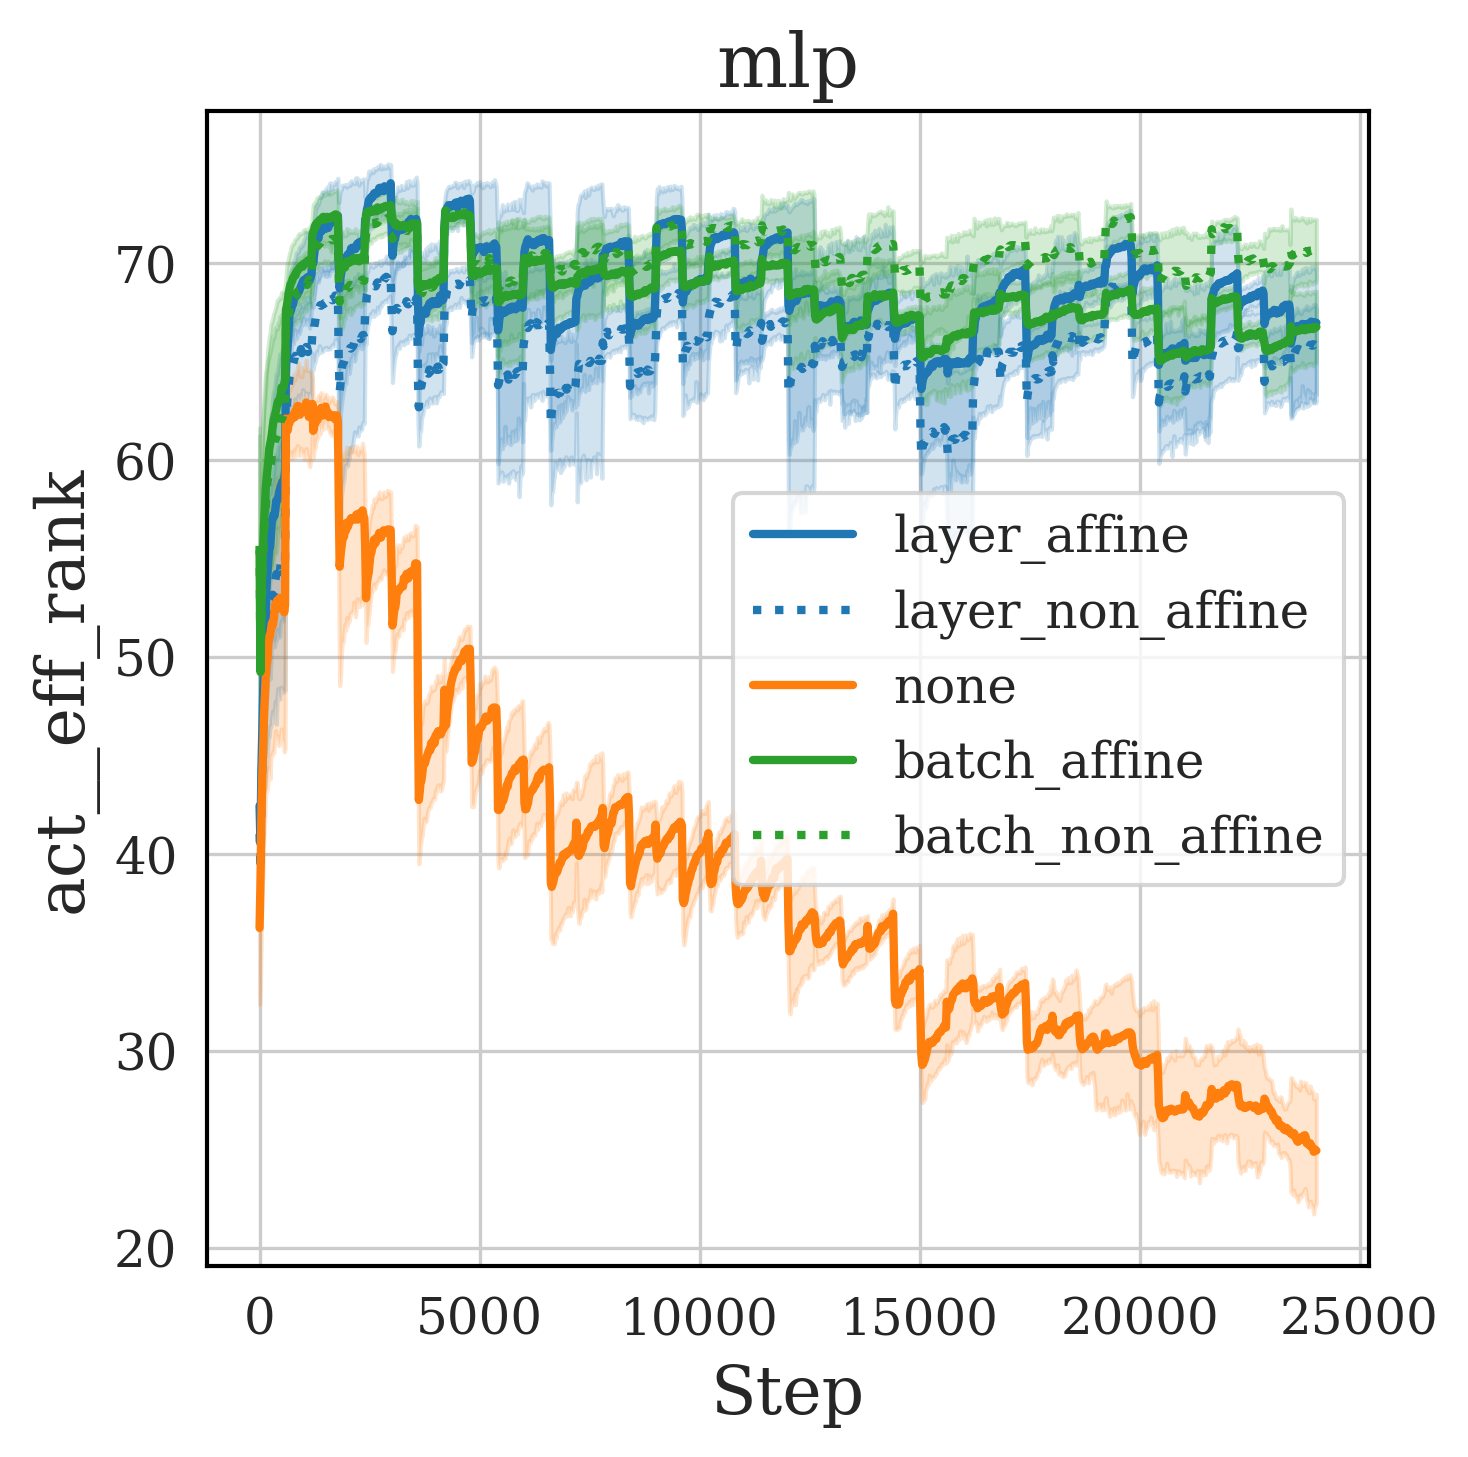
\includegraphics[width=0.24\linewidth]{paper/images/mlp_rankandnorm.png}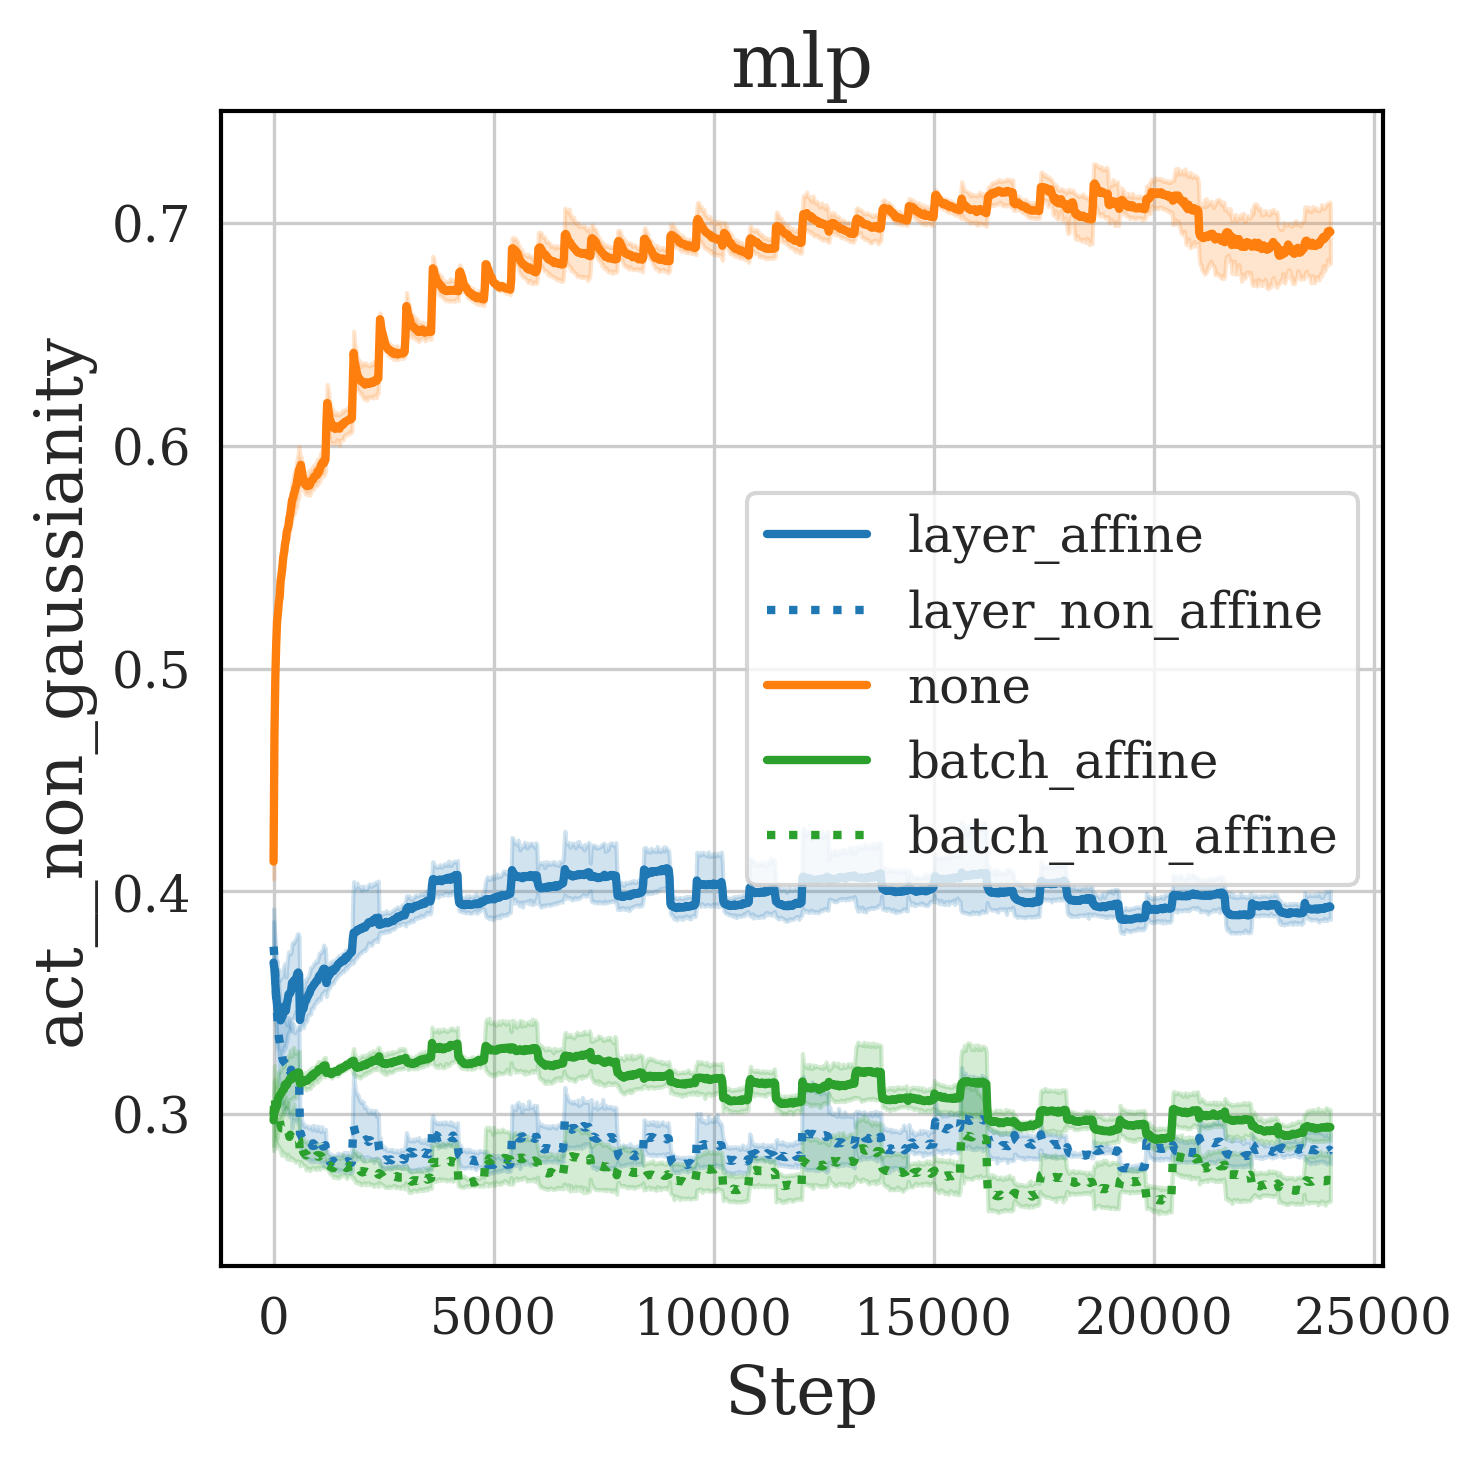
\includegraphics[width=0.24\linewidth]{paper/images/mlp_nonGaussnorm.png}
    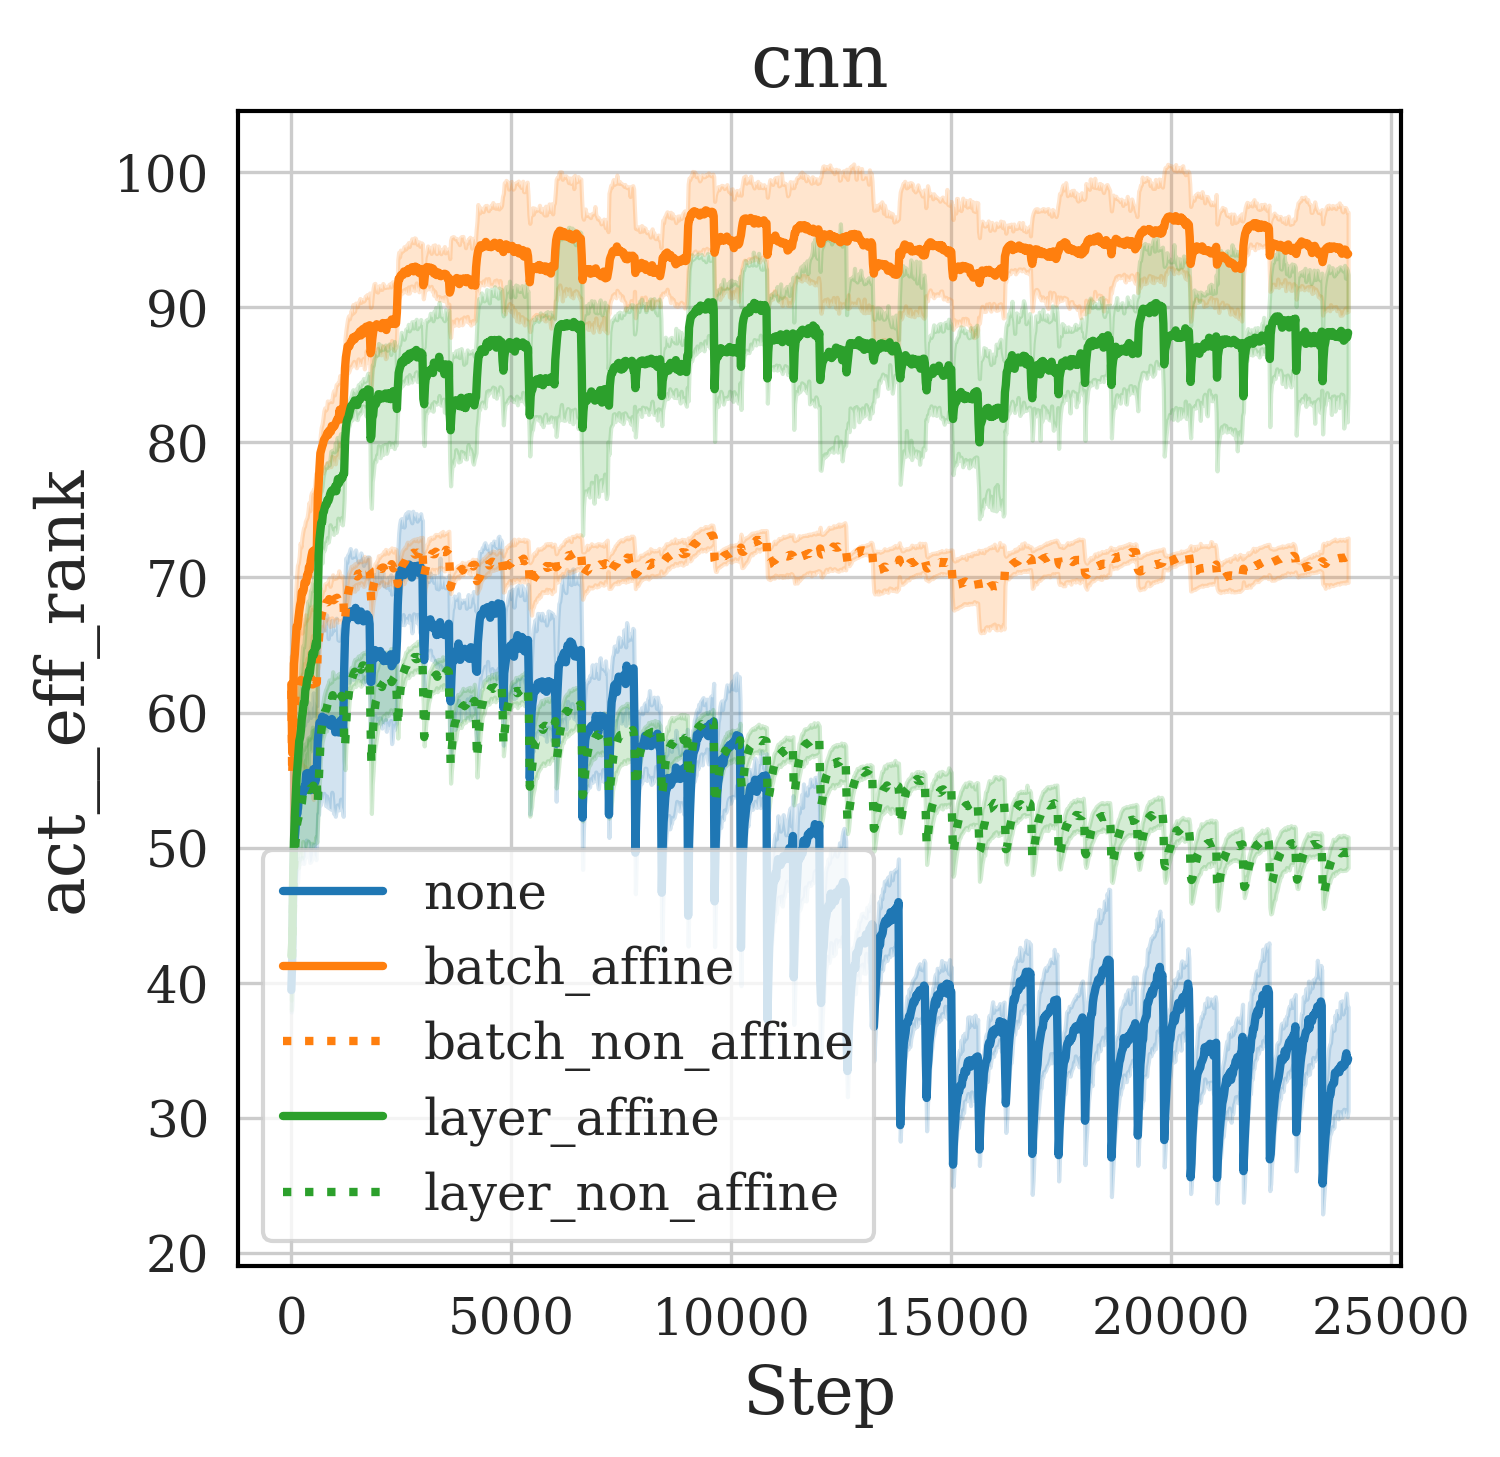
\includegraphics[width=0.24\linewidth]{paper/images/cnn_rankandnorm.png}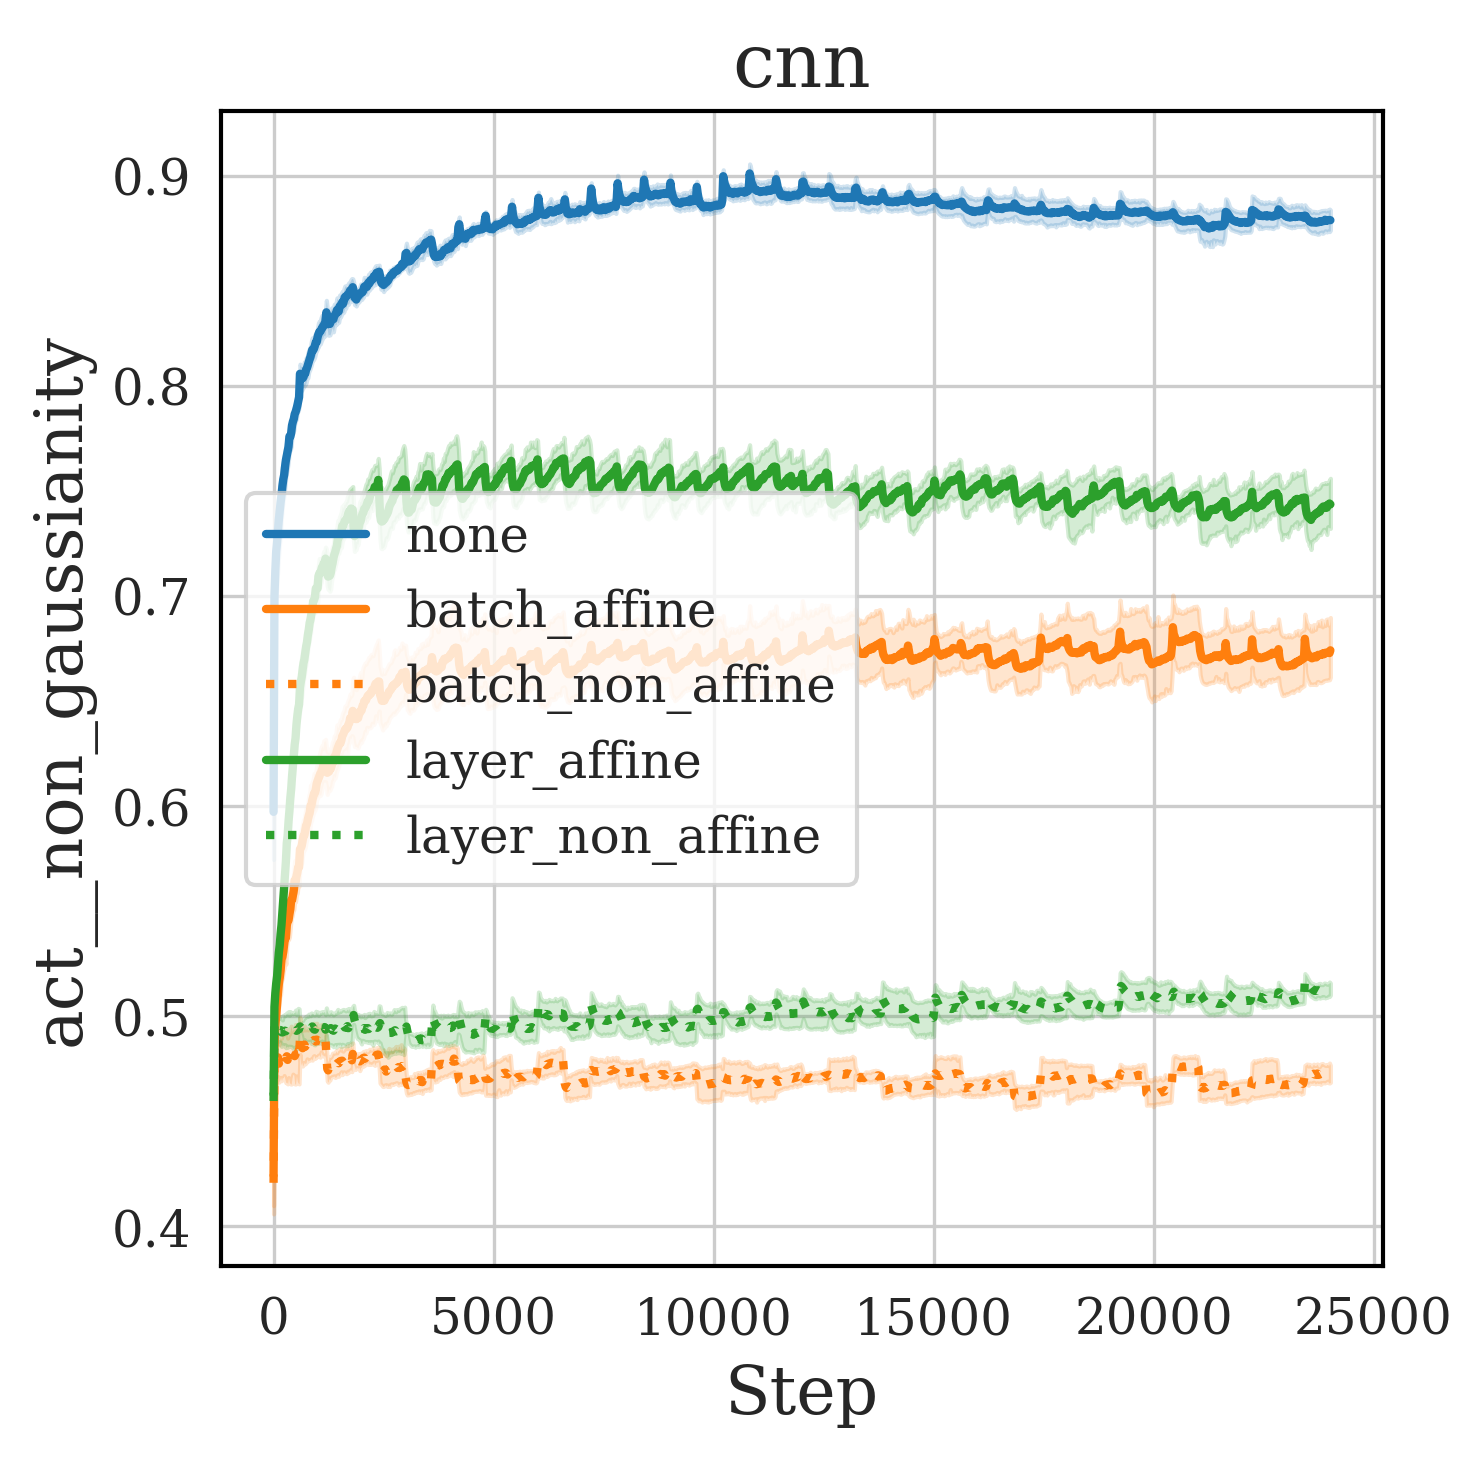
\includegraphics[width=0.24\linewidth]{paper/images/cnn_nonGaussnorm.png}

    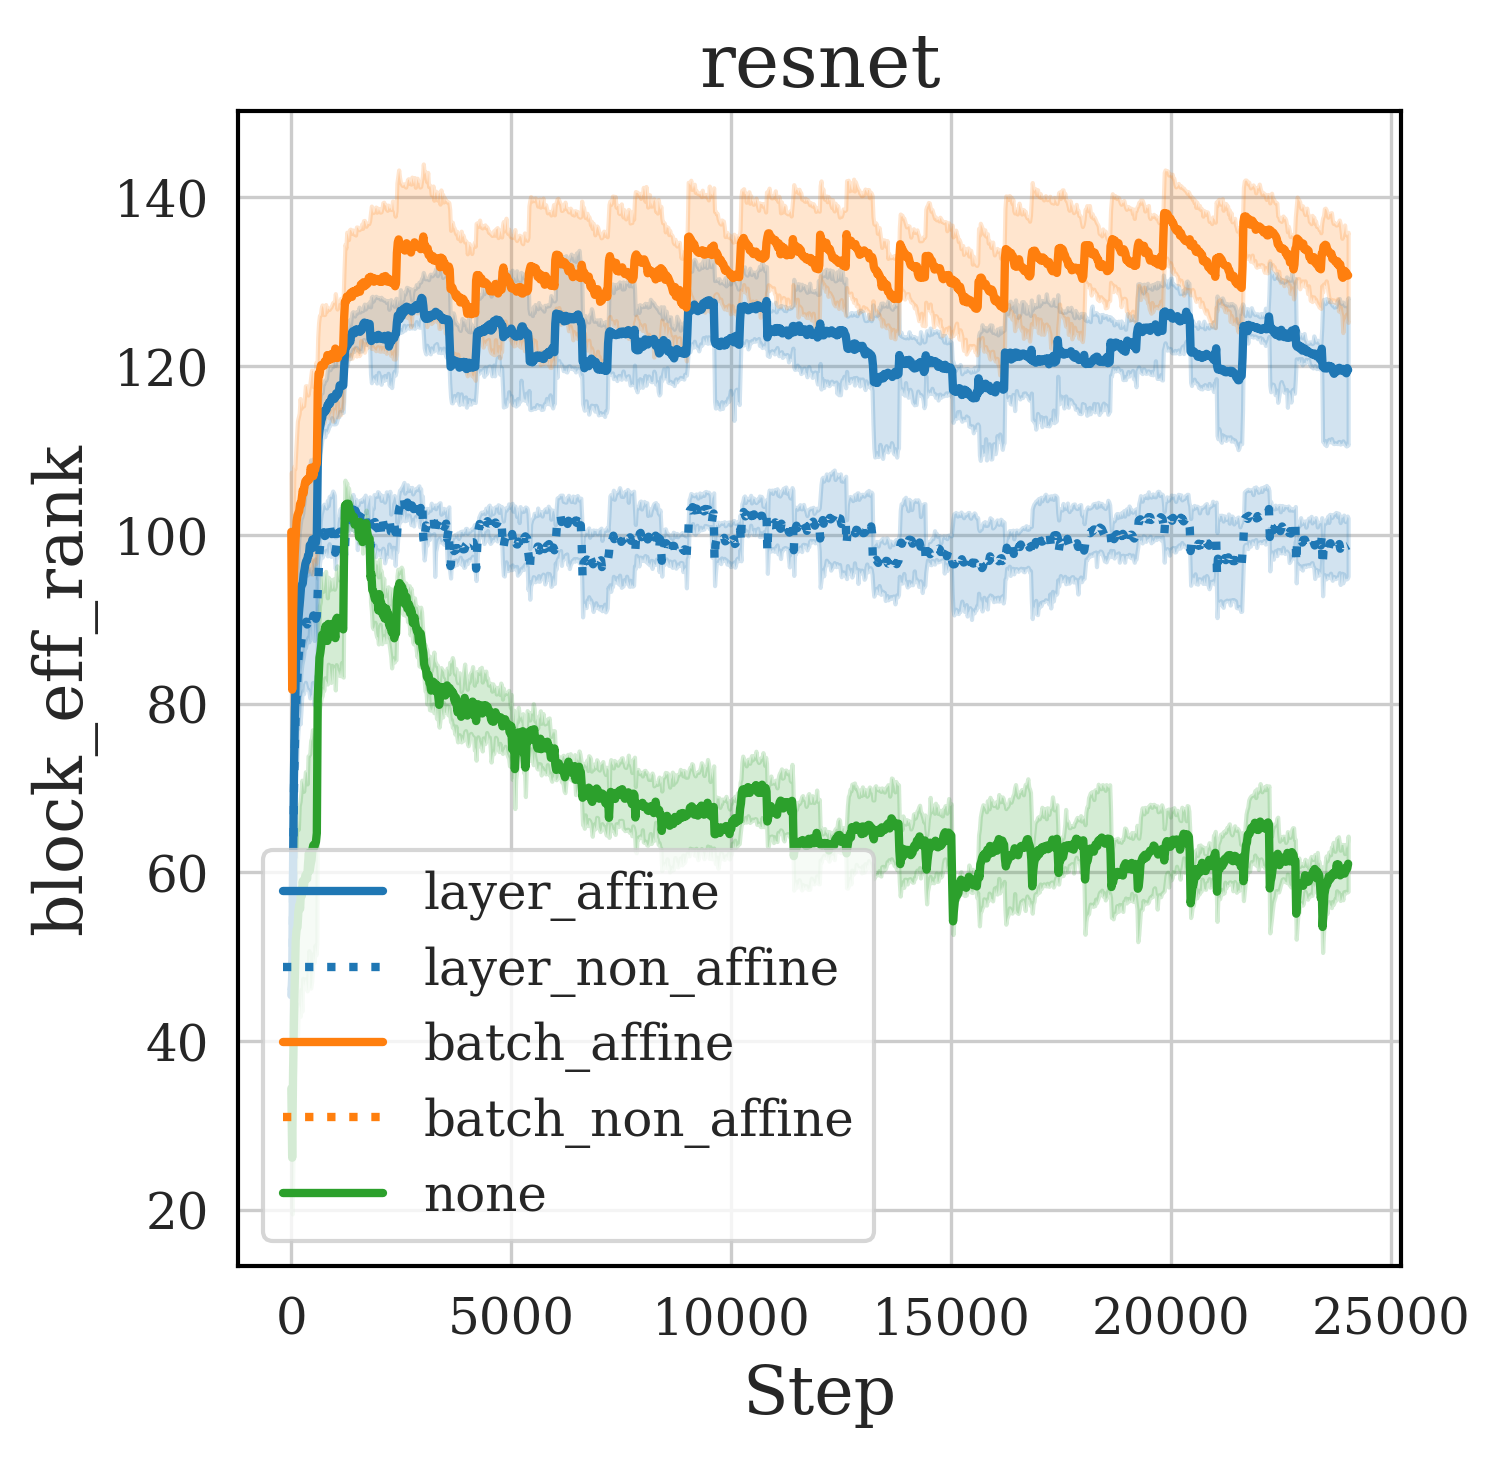
\includegraphics[width=0.24\linewidth]{paper/images/resnet_rankandnorm.png}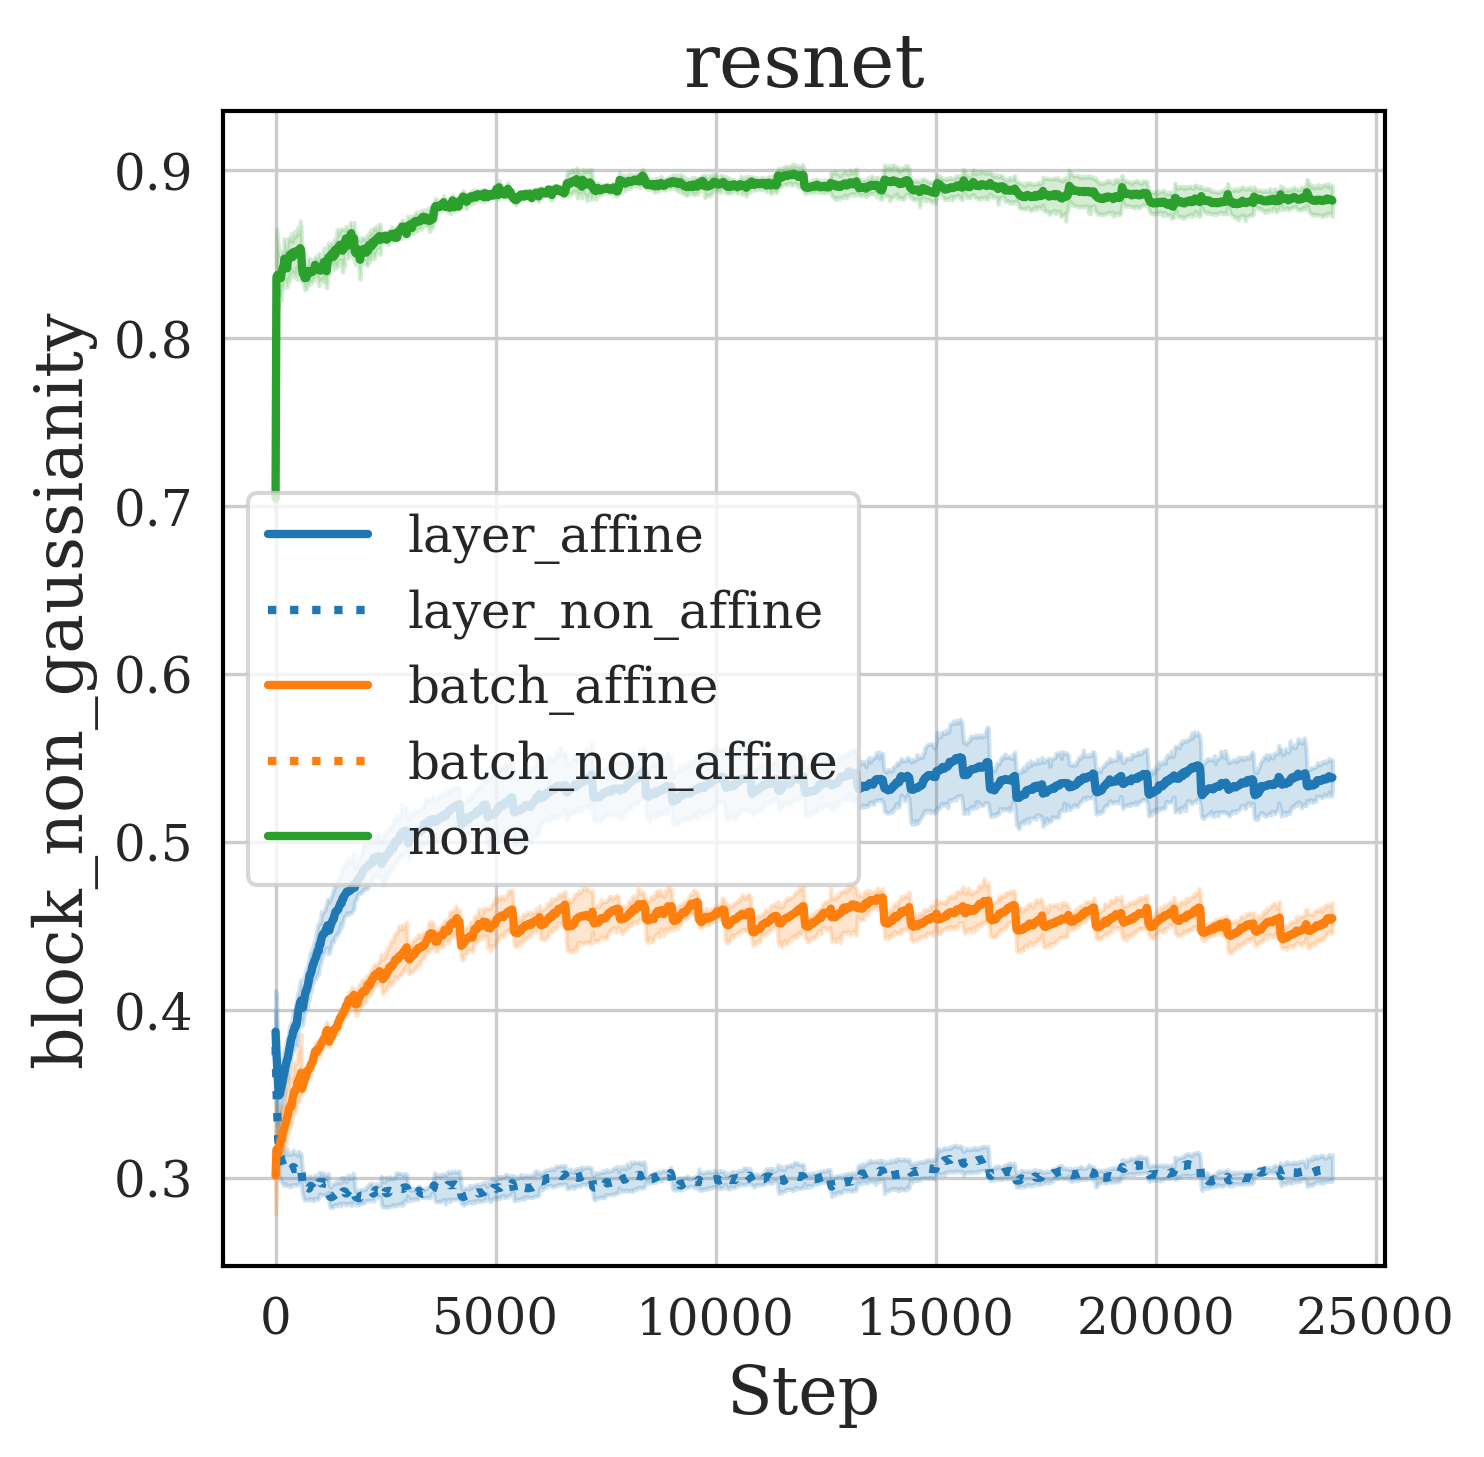
\includegraphics[width=0.24\linewidth]{paper/images/resnet_nonGaussnorm.png}
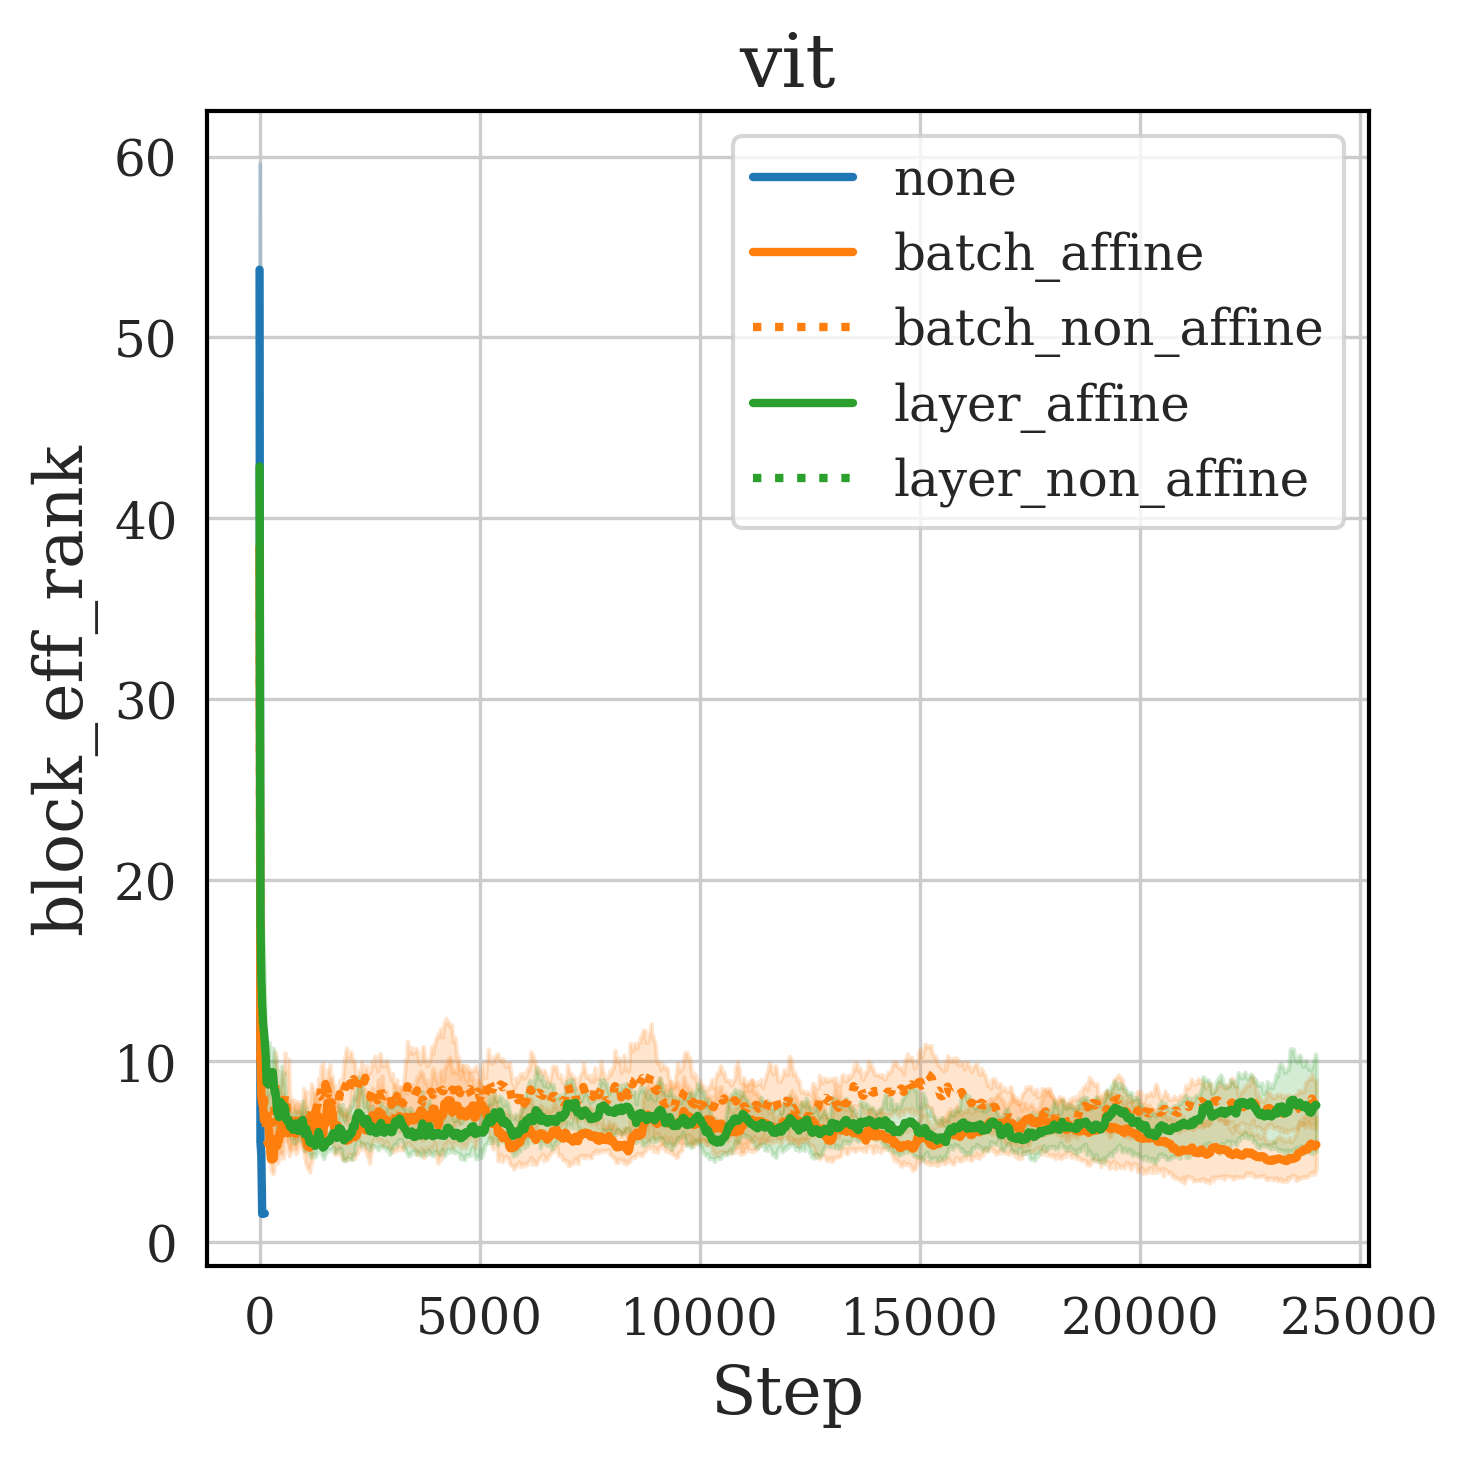
\includegraphics[width=0.24\linewidth]{paper/images/vit_rankandnorm.png}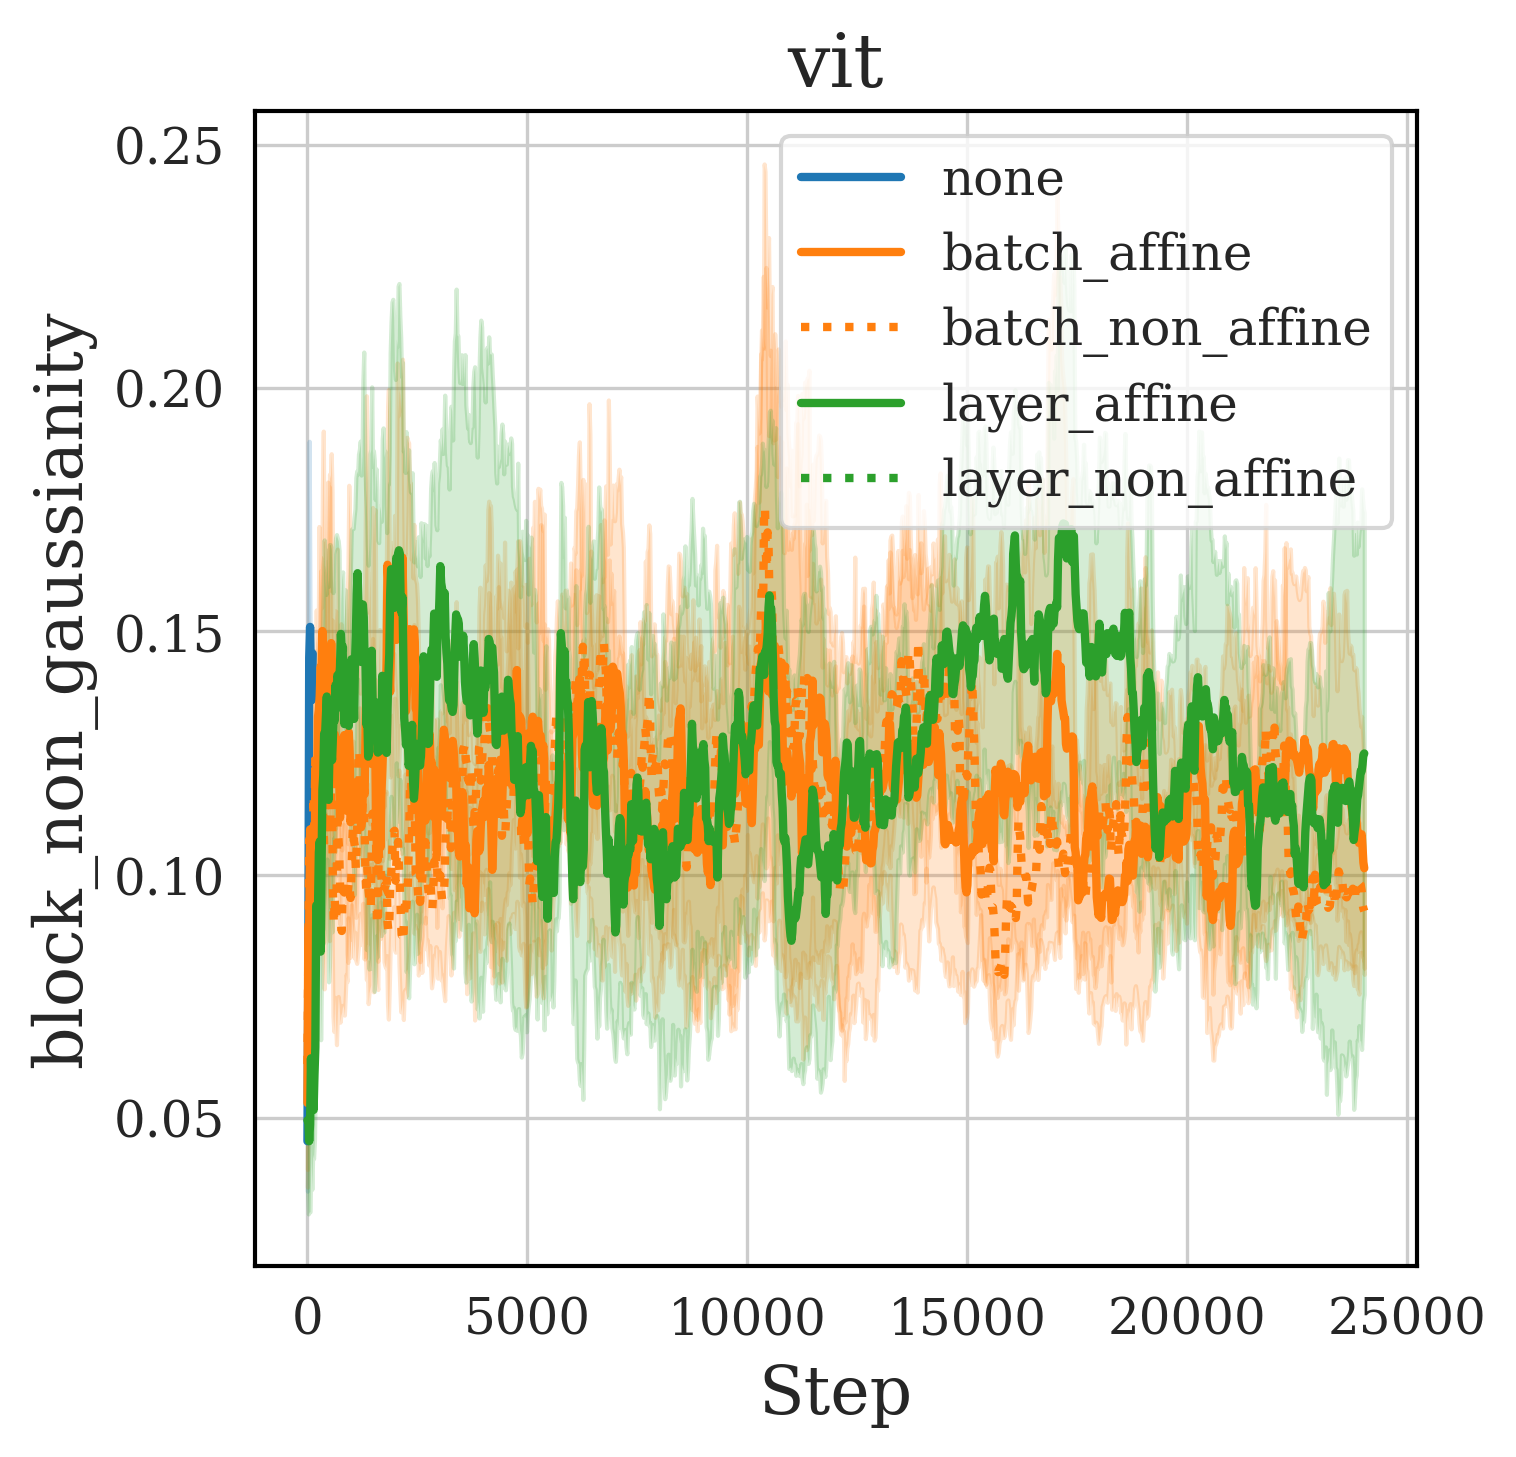
\includegraphics[width=0.24\linewidth]{paper/images/vit_nonGaussnorm.png}
    
    \caption{(Placeholder figure, not final) Effect of normalization on Effective Rank and Gaussianity. Dropout is 0. (Warning: The colours in different architectures do not have the same meaning)}
    \label{fig:norm-rank-nG}
\end{figure}

\begin{figure}[h!]
    \centering
    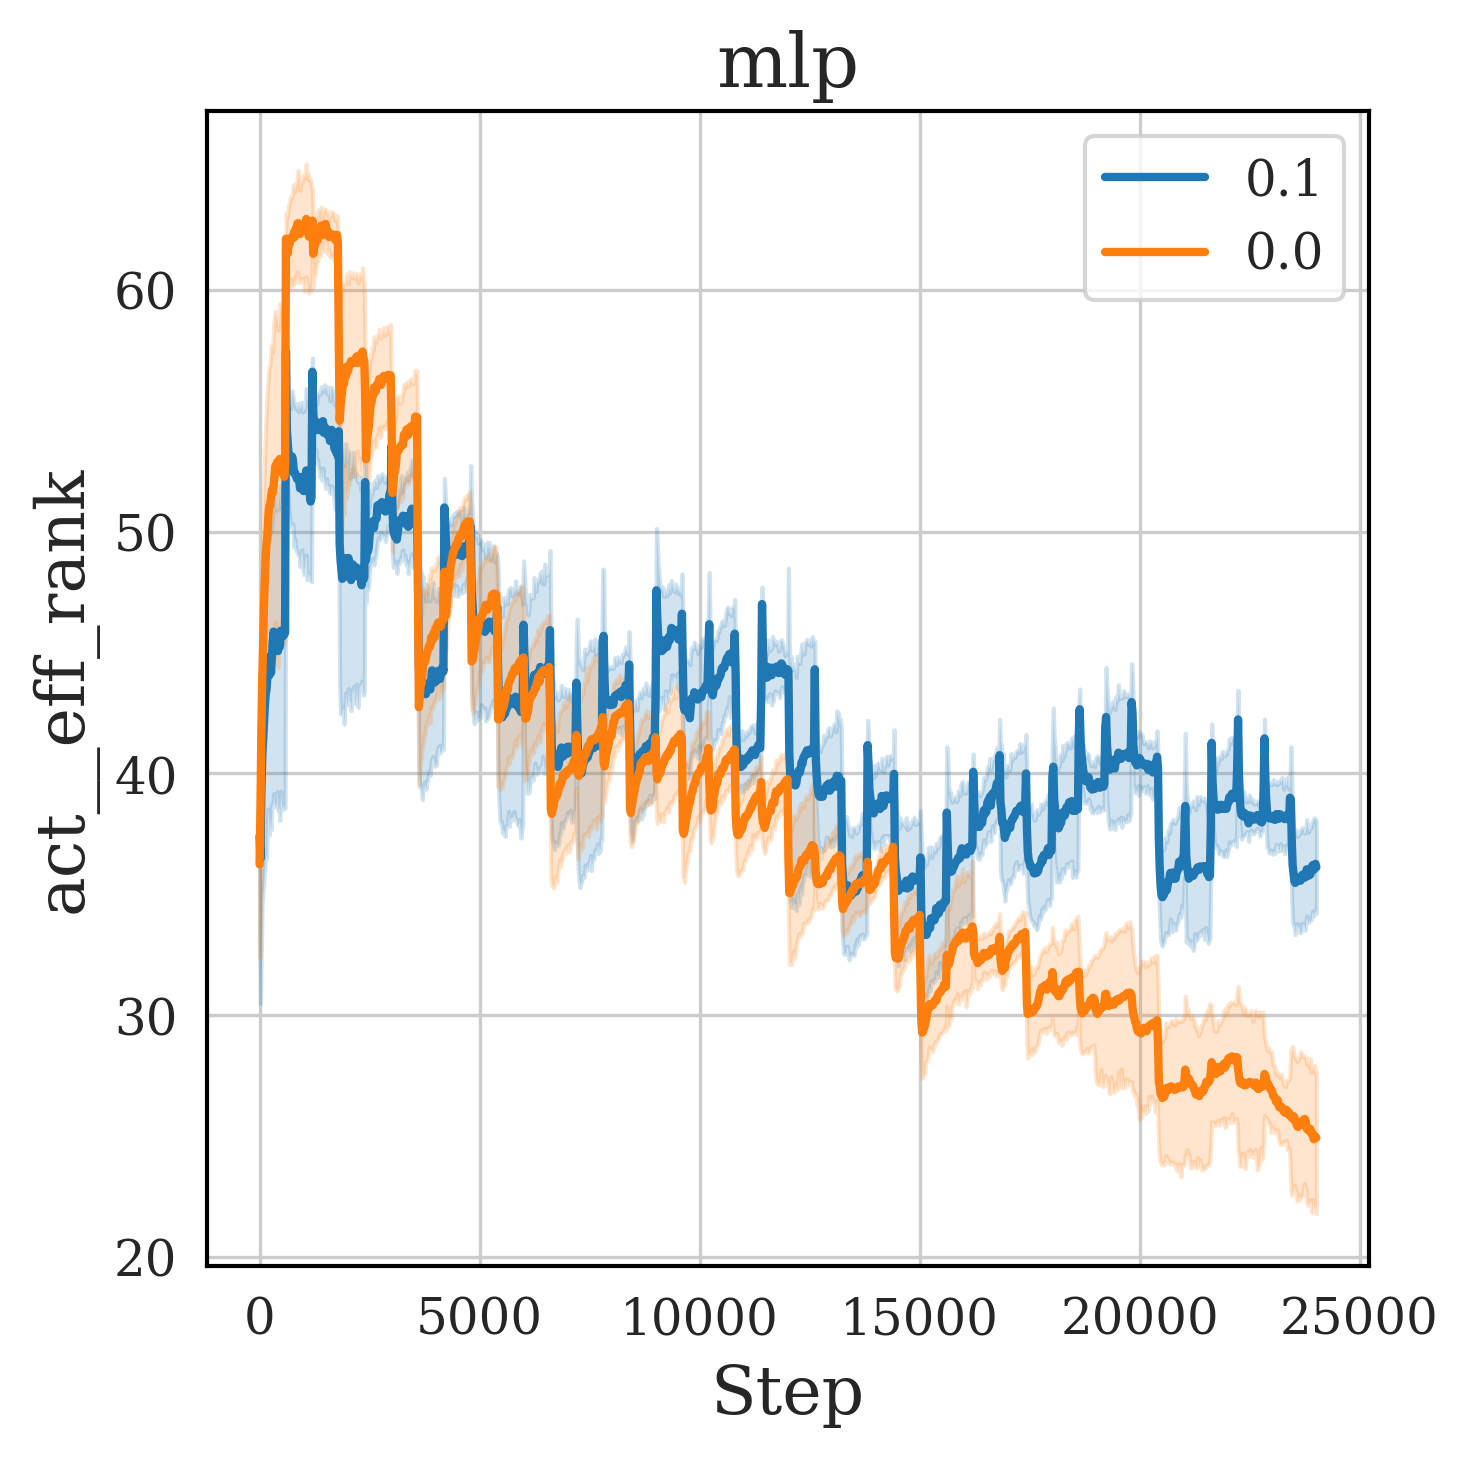
\includegraphics[width=0.24\linewidth]{paper/images/mlp_rankanddropout.png}    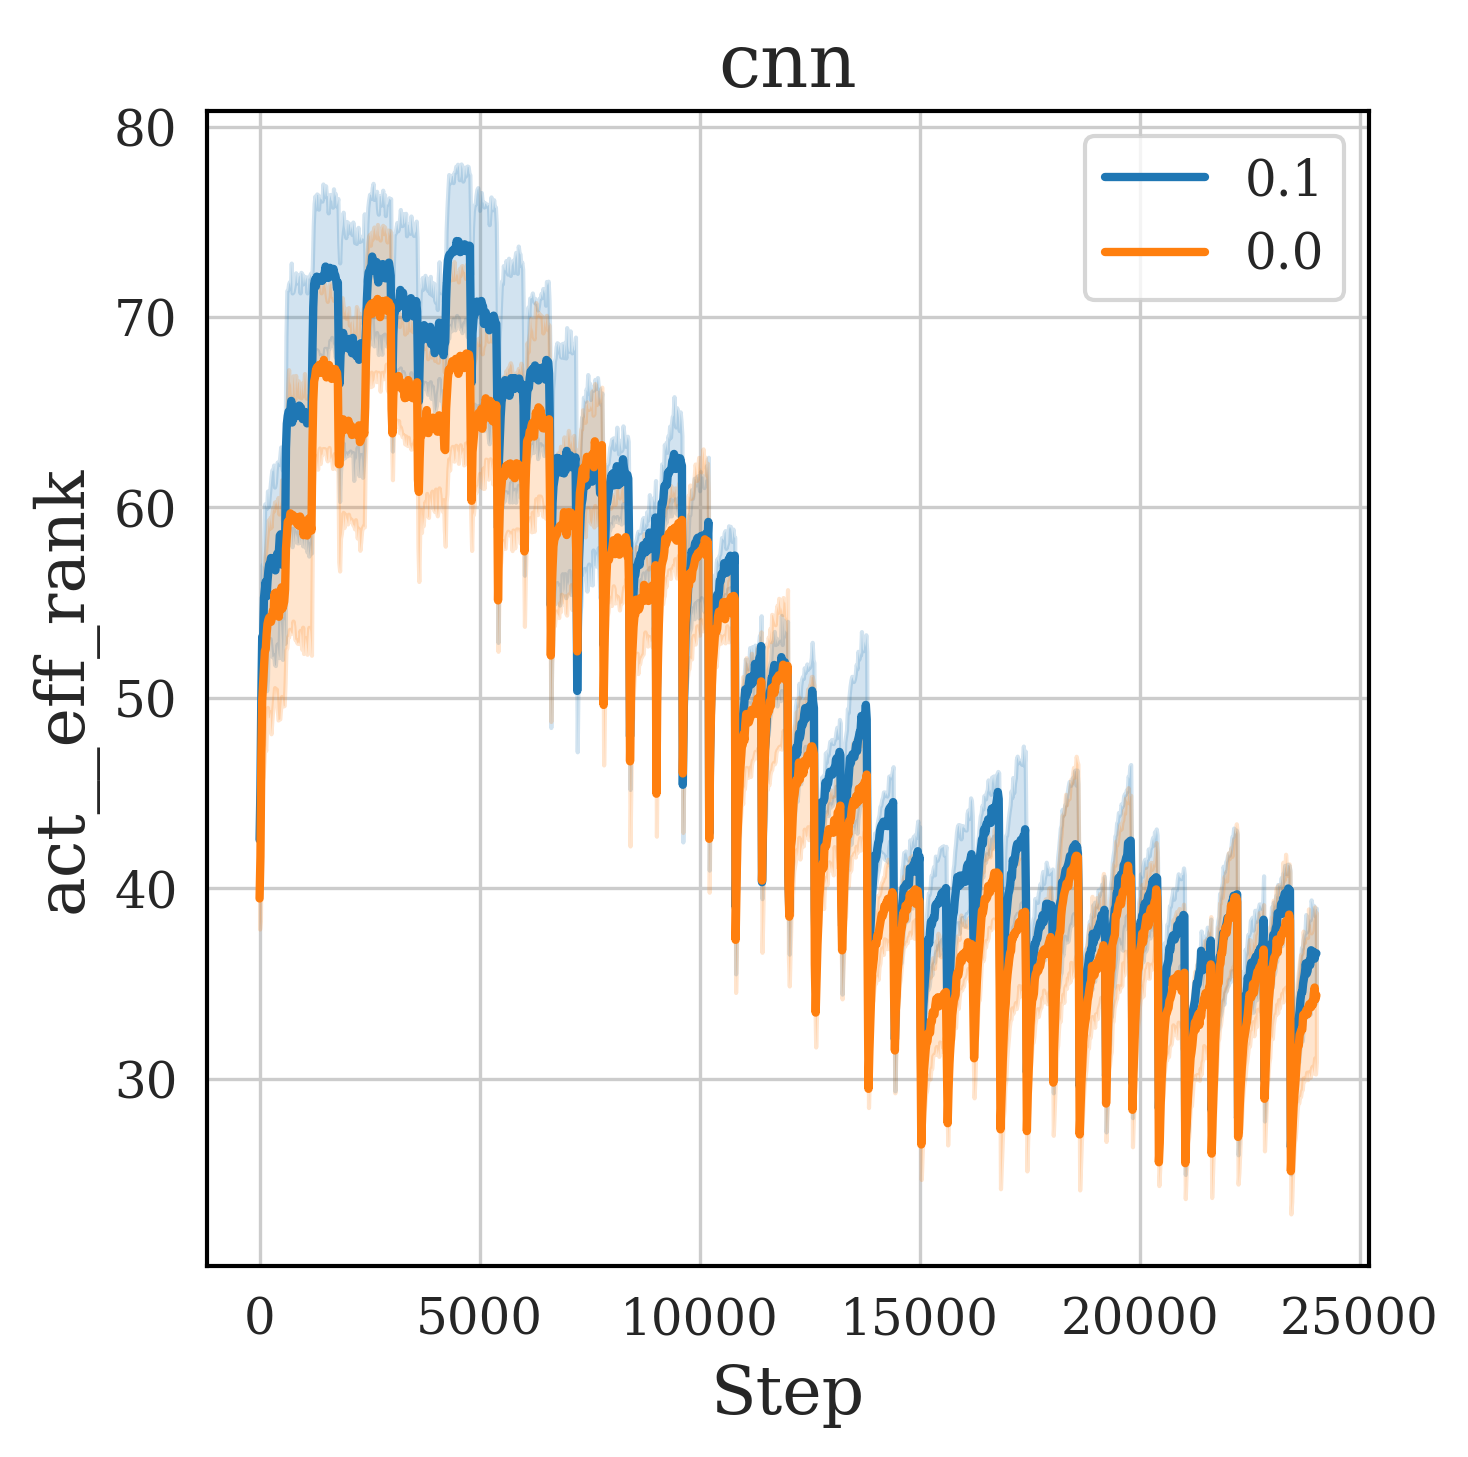
\includegraphics[width=0.24\linewidth]{paper/images/cnn_rankanddropout.png}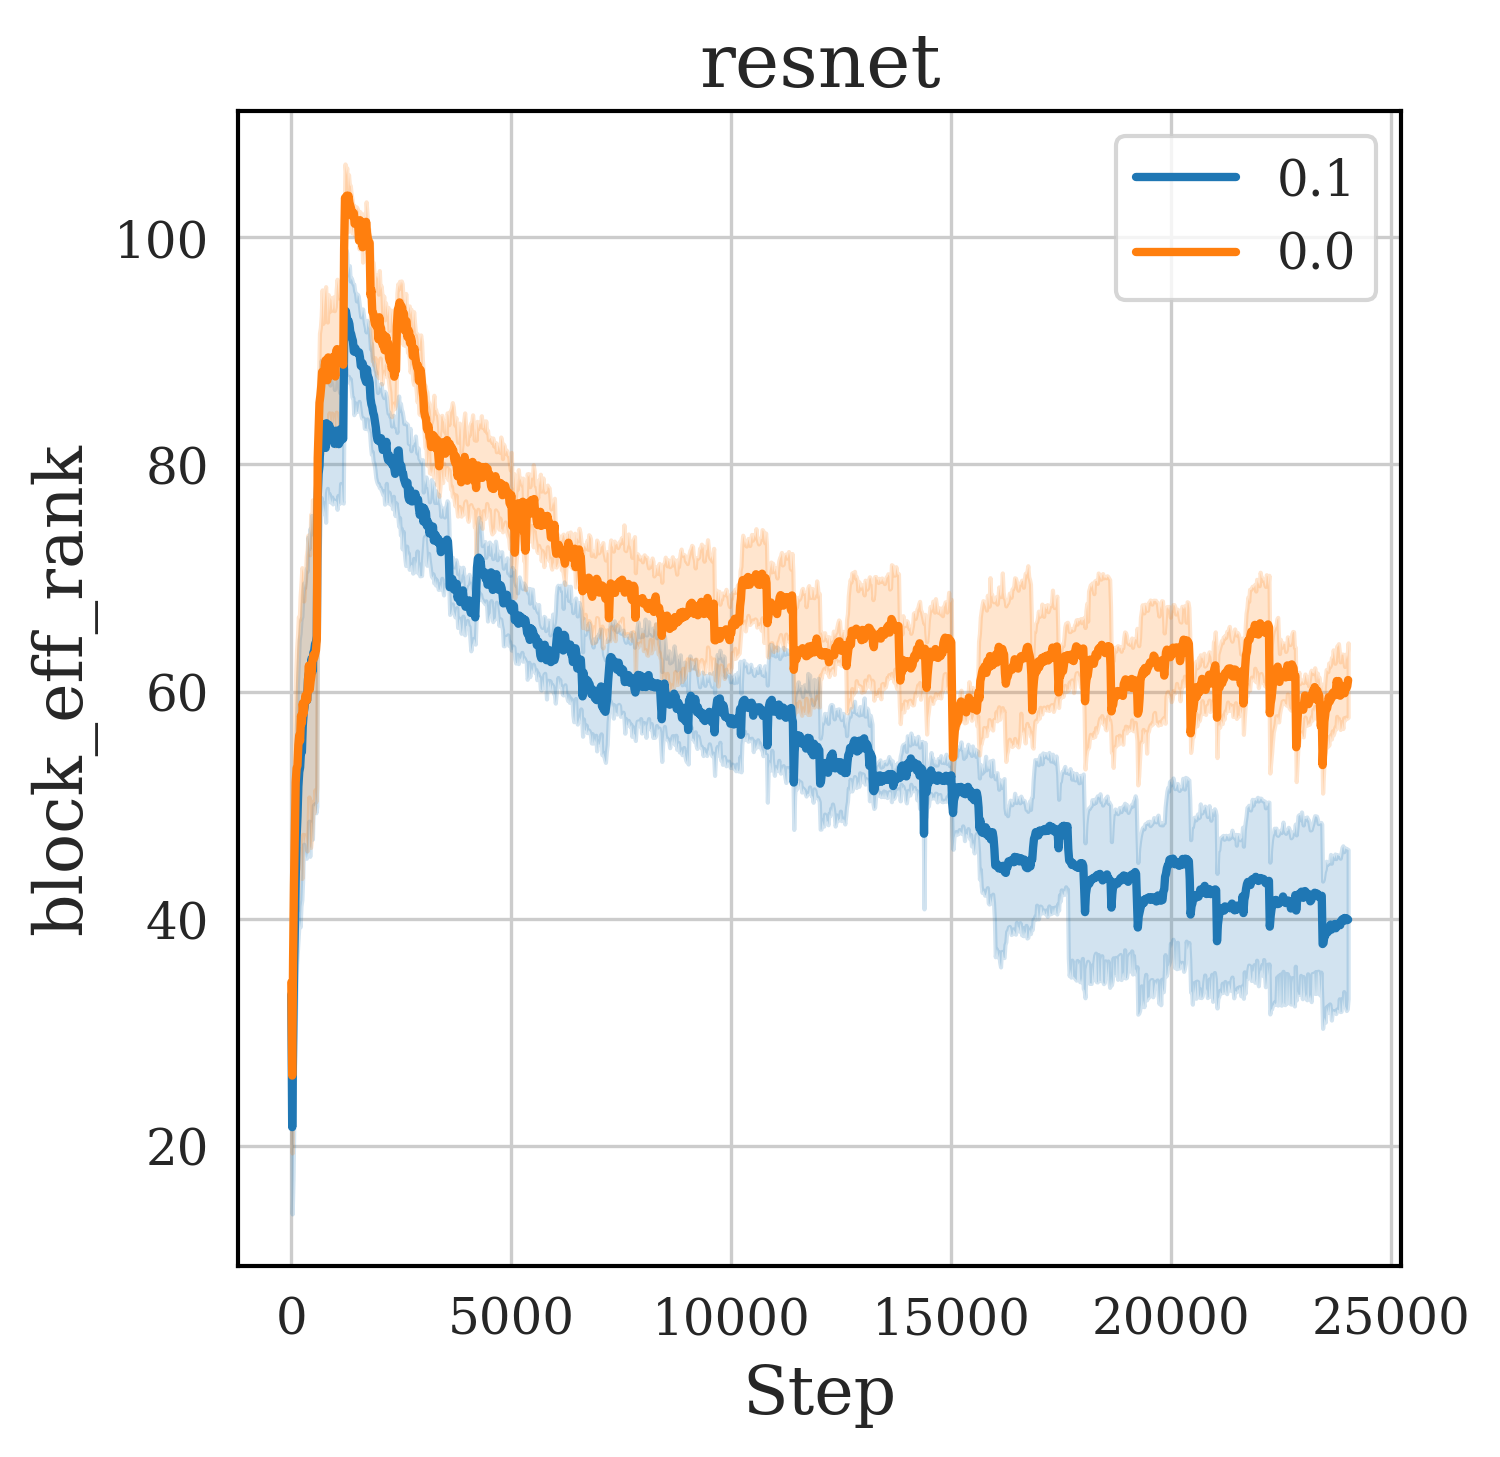
\includegraphics[width=0.24\linewidth]{paper/images/resnet_rankanddropout.png}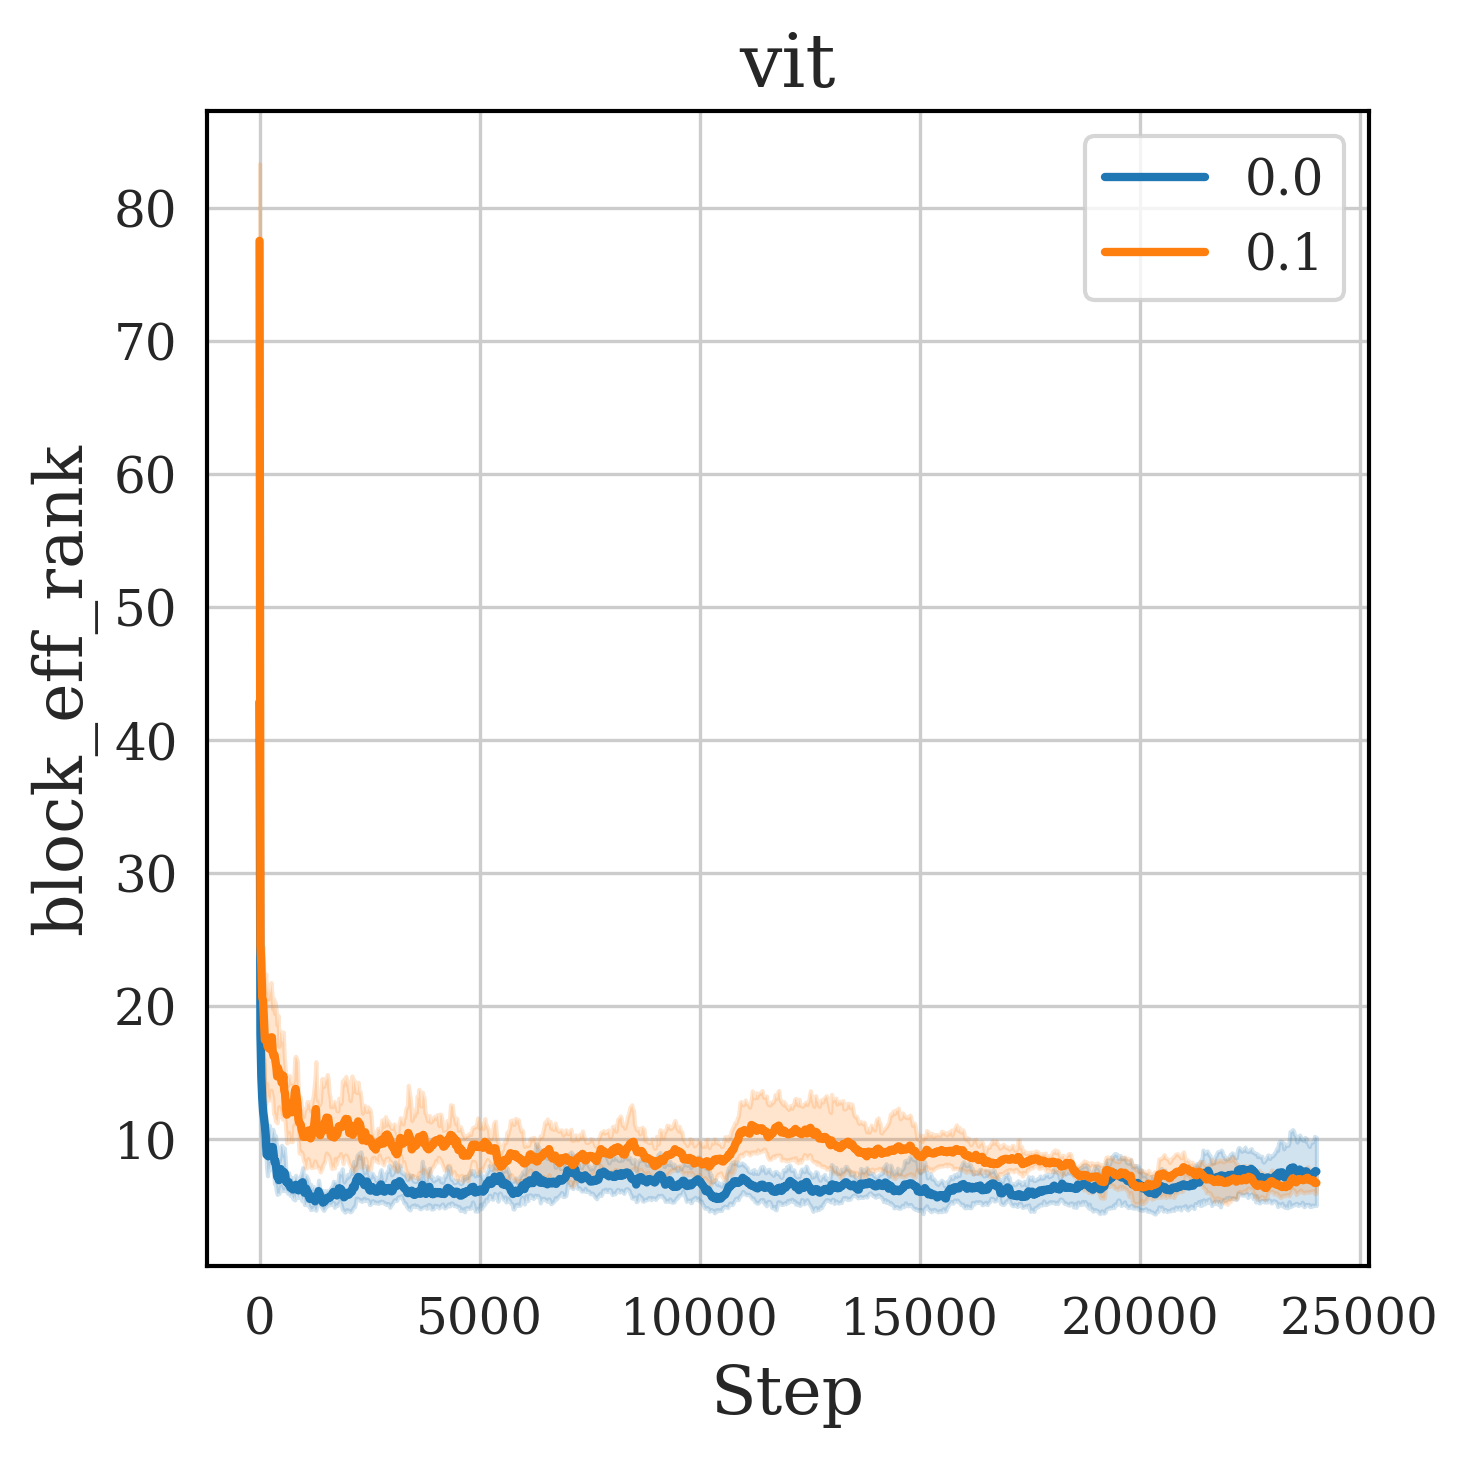
\includegraphics[width=0.24\linewidth]{paper/images/vit_rankanddropout.png}
    \caption{(Placeholder figure, not final) Effect of dropout on Effective Rank. No normalization applied, except layer on vit.}
    \label{fig:dropout-rank}
\end{figure}

\subsection{Escaping a Plasticity-Loss Manifold}

If a network's parameters $\theta(t)$ have converged to a stable loss-of-plasticity manifold $\mathcal{M}$, gradient descent alone cannot facilitate escape. However, perturbations or noise injection might allow the trajectory to leave the manifold if the curvature permits.

\begin{corollary}[Perturbation dynamics]
\label{cor:perturb}
Suppose the parameters are at a point $\theta_0 \in \mathcal{M}$. Consider a small perturbation $\varepsilon v$ in a direction $v$ normal to the manifold at $\theta_0$, i.e., $v \in N_{\theta_0}\mathcal{M}$ with $\|v\|=1$. The initial state after perturbation is
\[
\theta(0)=\theta_0+\varepsilon v,\qquad \text{where } \varepsilon \ll 1.
\]
The initial rate of change of the squared distance from the manifold $\mathcal{M}$ under gradient flow (Equation~\ref{eq:grad_flow}) can be approximated. Let $d(\theta, \mathcal{M})^2$ denote the squared Euclidean distance from $\theta$ to the closest point on $\mathcal{M}$. Then, the initial dynamics perpendicular to the manifold are governed by the Hessian:
\(
\frac{d}{dt}\left.\mathrm{dist}^2(\theta(t),\mathcal{M})\right|_{t=0} \approx \frac{d}{dt} \|\theta(t) - \theta_0\|^2 \Big|_{t=0} = -2 (\theta(0)-\theta_0)^\top \nabla_\theta \Loss(\theta(0)) \approx -2 \varepsilon v^\top (\nabla_\theta \Loss(\theta_0) + \varepsilon \nabla_\theta^2 \Loss(\theta_0) v)
\)
Since $\nabla_\theta \Loss(\theta_0)$ is tangent to $\mathcal{M}$ (Definition~\ref{def:lop}(a)) and $v$ is normal, $v^\top \nabla_\theta \Loss(\theta_0) = 0$. Thus,
\[
\frac{d}{dt}\left.\mathrm{dist}^2(\theta(t),\mathcal{M})\right|_{t=0} \approx -2\varepsilon^2\,v^\top\nabla_\theta^2\Loss(\theta_0)v + O(\varepsilon^3).
\]
The distance from the manifold will initially increase (i.e., plasticity is potentially recovered) if and only if there exists a normal direction $v$ with negative curvature, $v^\top\nabla_\theta^2\Loss(\theta_0)v < 0$.
\end{corollary}

\giulia{Maybe another way to explain the benefit of noise injection is to say that high-dimensional independent noise increases the rank of the features, (intuitively) because two correlated features will be perturbed independently?}
This corollary explains why techniques involving noise injection or periodic re-initialization of parts of the network, such as the continual backpropagation algorithm proposed by \cite{dohare2024loss} , can sometimes succeed in restoring plasticity. If the manifold is only stable (positive curvature in all normal directions, Equation~\ref{eq:stable}), noise alone won't help escape via gradient descent. However, if the manifold is of saddle type (Equation~\ref{eq:saddle}), perturbations along directions of negative curvature can initiate escape trajectories. If the manifold is unstable (Equation~\ref{eq:unstable}), any perturbation will lead to escape. This highlights the importance of the loss landscape's geometry around these manifolds.


\begin{figure}[h!]
    \centering
    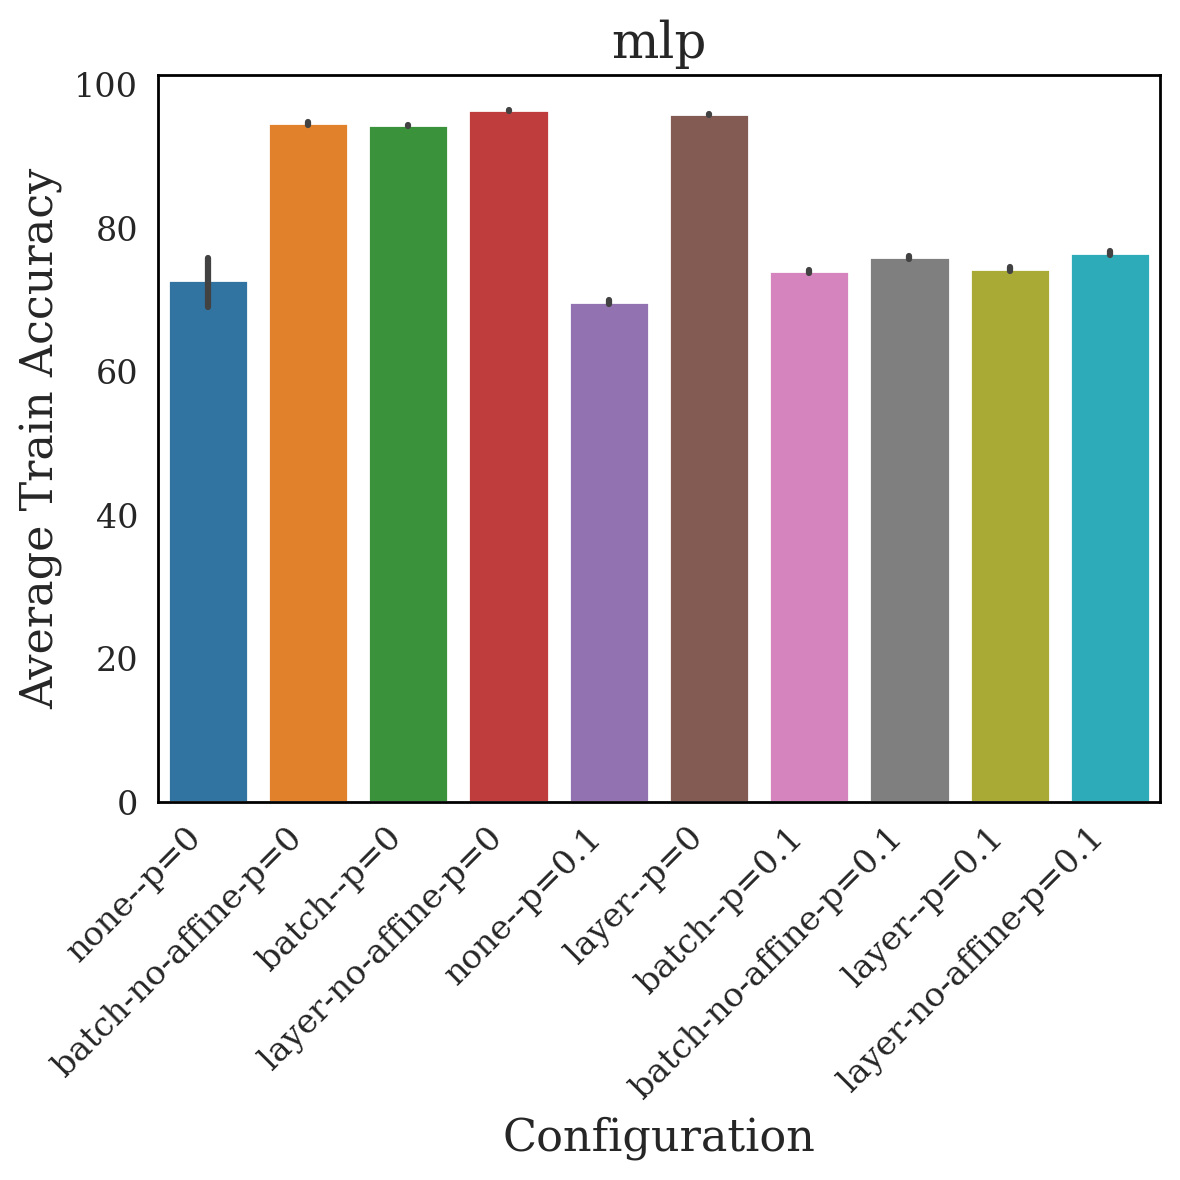
\includegraphics[width=0.33\linewidth]{paper/images/mlp_config_finalperf.png}
    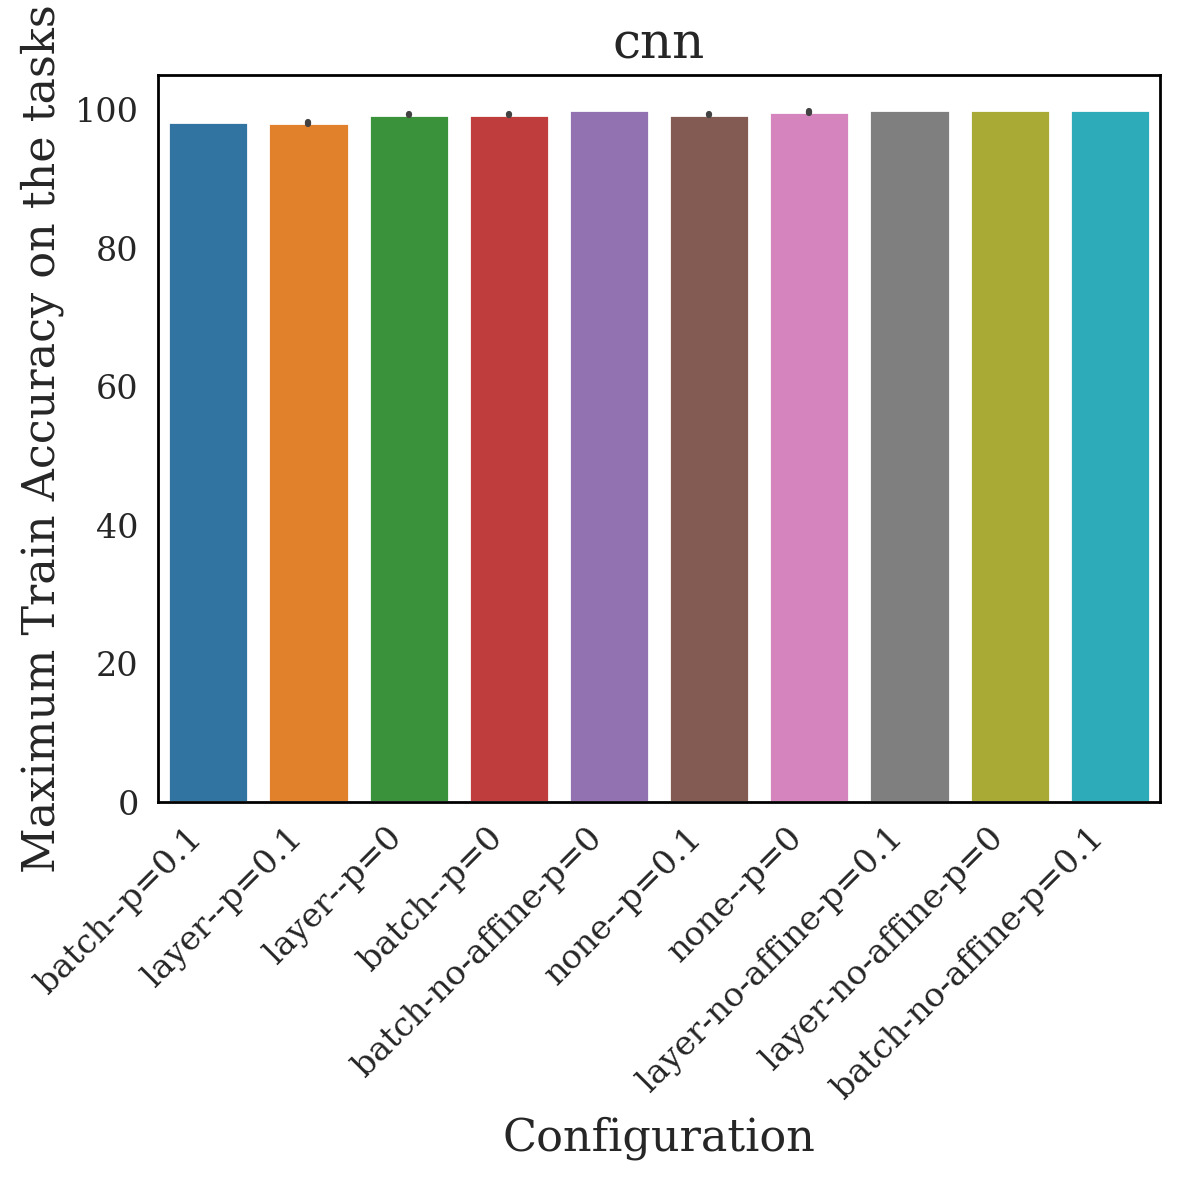
\includegraphics[width=0.33\linewidth]{paper/images/cnn_config_finalperf.png}
    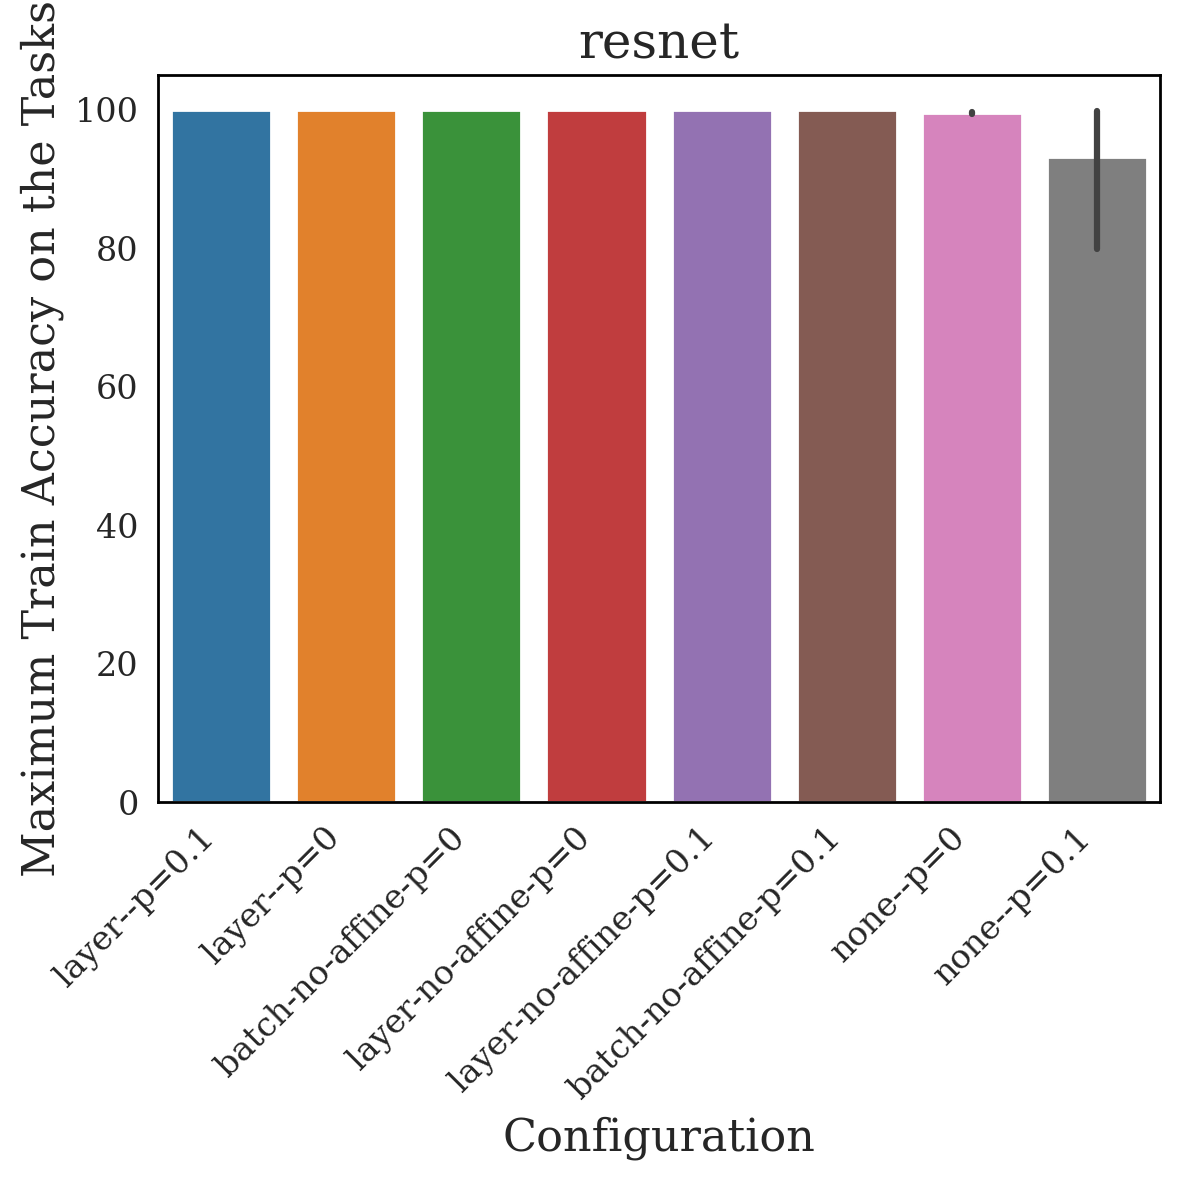
\includegraphics[width=0.33\linewidth]{paper/images/resnet_config_finalperf.png}
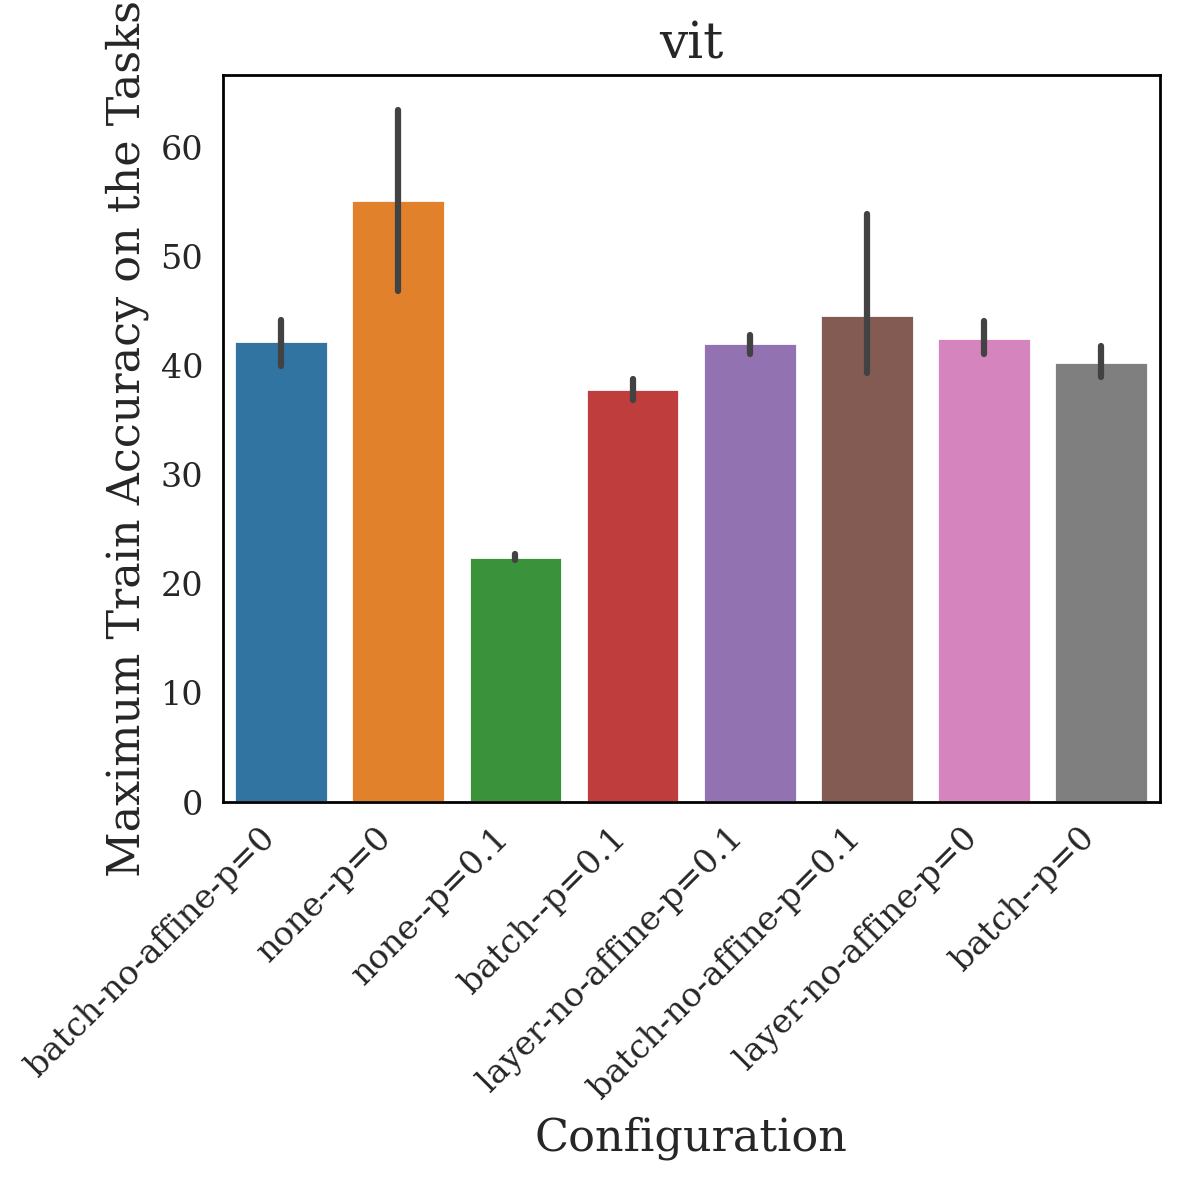
\includegraphics[width=0.33\linewidth]{paper/images/vit_config_finalperf.png}
    
    \caption{(Placeholder figure, not final - can become a table) Summary of final performance dependent on normalization and dropout. The y axis is the maximum train accuracy reached on each task, averaged over tasks. The standard deviation is over all runs with the same configuration.}
    \label{fig:mlp-config-finalperf}
\end{figure}

\section{Empirical Evaluation (Planned)}
\label{sec:experiments}
\giulia{I would split this section up, leaving the experimental evidence in the section where the hypotheses and theoretical results are discussed.}

To validate the theoretical constructs presented, a series of empirical investigations are planned. These experiments will aim to provide concrete evidence for the proposed mechanisms of plasticity loss and the effectiveness of mitigation strategies. The core hypotheses to be tested are:
\begin{itemize}
    \item \textbf{Emergence of Plasticity Loss Symptoms:} We will train standard neural network architectures (e.g., MLPs, ResNets) on continual learning benchmarks (e.g., sequences of image classification tasks derived from CIFAR-100 or ImageNet, similar to setups in \cite{dohare2024loss}). We will track metrics over extended training periods, specifically measuring:
        \begin{itemize}
            \item Performance on the current task (as a measure of plasticity).
            \item The percentage of saturated/dead units (e.g., ReLUs with zero output across a batch).
            \item The effective rank of representations in hidden layers (e.g., using participation ratio of singular values of the activation Gram matrix \cite{huh2022lowrank}).
        \end{itemize}
        We expect to observe a decrease in current task performance correlated with an increase in dead units and a decrease in effective rank over long training horizons, confirming the link between these symptoms and plasticity loss.

    \item \textbf{The Cloning Hypothesis:} To directly test Proposition~\ref{prop:cloned}, we will construct a ``wide'' network $\mathcal{G}$ initialized with weights satisfying the cloning conditions relative to a smaller ``narrow'' network $G$. We will train $\mathcal{G}$ on a task sequence and monitor its parameter trajectory. We hypothesize that the parameters $\mathcal{W}(t)$ will remain confined to the affine subspace predicted by the proposition, and the network's performance will mirror that of the smaller network $G$ trained independently. We will measure the distance of $\mathcal{W}(t)$ from this subspace.

    \item \textbf{Escaping Cloned Subspace:} We will repeat the cloning experiment but introduce mechanisms designed to break the symmetry or perturb the trajectory, as suggested by Section~\ref{sec:mitigate}. Specifically, we will compare the baseline cloned network to variants incorporating:
        \begin{itemize}
            \item Dropout \cite{srivastava2014dropout}.
            \item Explicit noise injection into gradients or weights during back-propagation (inspired by Corollary~\ref{cor:perturb} and \cite{dohare2024loss}).
        \end{itemize}
        We hypothesize that these interventions will cause the parameter trajectory $\mathcal{W}(t)$ to deviate significantly from the cloned subspace, potentially leading to improved plasticity (higher performance on later tasks) compared to the baseline cloned network. Measurements will include distance from the manifold and task performance.
\end{itemize}
These experiments are designed to bridge the gap between our theoretical framework and observable phenomena in deep continual learning.

\section{Discussion and Open Questions}

This work provides a mathematical framework, grounded in dynamical systems theory, for understanding the phenomenon of loss of plasticity in deep neural networks trained with gradient-based methods. By defining loss of plasticity manifolds and identifying mechanisms like activation saturation (frozen units) and representational redundancy (cloned units) that lead to stable confinement within these manifolds, our analysis connects and provides a potential unifying explanation for several previously observed empirical phenomena, including dead ReLUs \cite{nair2010rectified}, aspects of neural collapse related to representational degeneracy \cite{papyan2020prevalence}, and issues arising from weight duplication or symmetry \cite{huh2022lowrank}.

A key implication of our analysis is the inherent tension between desirable properties for static learning and the requirements for continual adaptation. Low-rank representations and simplicity bias, often linked to better generalization on fixed datasets \cite{huh2022lowrank, papyan2020prevalence, zhang2017understanding}, appear to be manifestations of the network settling into lower-dimensional subspaces. While beneficial for compressing information relevant to a static task, this very compression hinders the ability to learn new, potentially orthogonal information, thus causing loss of plasticity as observed by \cite{dohare2024loss}.

This framework raises several critical questions for future research aimed at achieving truly continual learning:

\begin{itemize}[nosep]
    \item \textbf{Designing Effective Continual Randomization:} While initial randomness is crucial, it gets consumed. How can we design \emph{ongoing} randomization schemes that effectively prevent trajectories from settling into stable plasticity-loss manifolds? Simple dropout \cite{srivastava2014dropout} or the periodic re-initialization proposed in continual backpropagation \cite{dohare2024loss} are steps in this direction, but can we develop adaptive noise injection or re-sampling strategies guided by online measurements of plasticity or manifold proximity?
    \item \textbf{Interaction with Advanced Optimizers:} How do optimization methods beyond first-order gradient descent interact with these manifolds? Can second-order methods, which utilize Hessian information (related to curvature, Corollary~\ref{cor:perturb}), detect and actively avoid or escape these stable regions? Could meta-gradient approaches, which adapt learning rules themselves (e.g., Sutton's early work on IDBD \cite{sutton1992gain}), learn strategies to maintain plasticity by navigating away from detrimental subspaces? 
    \item \textbf{Characterizing Non-Linear Manifolds:} Our analysis focused on mechanisms leading to (affine) linear subspaces (frozen parameters, cloned units). Is it possible for plasticity loss to occur via trapping in more complex, non-linear stable manifolds? Identifying and characterizing such manifolds would require extending the current dynamical systems analysis.
    \item \textbf{Plasticity in Parameter-Efficient Fine-Tuning (PEFT):} Methods like LoRA \cite{hu2021lora} and Adapters \cite{houlsby2019parameter} achieve efficiency by restricting updates to low-dimensional parameter subspaces.[18, 19, 20, 21] Does this inherent low-dimensionality make PEFT methods particularly susceptible to a form of plasticity loss where the adapter subspace itself saturates or collapses during continual learning? How can plasticity be maintained within these parameter-efficient frameworks? Recent work exploring Parameter-Efficient Continual Fine-Tuning (PECFT) is beginning to address this, but a deeper theoretical understanding of plasticity dynamics within PEFT subspaces is needed. The efficiency gains of PEFT might fundamentally trade off against long-term adaptability, representing a critical research frontier.
\end{itemize}

Addressing these questions is crucial for developing AI systems capable of lifelong learning and adaptation in complex, evolving environments.

\section{Broader Impacts}
This research contributes to the fundamental understanding of limitations inherent in current deep learning paradigms, particularly concerning their ability to learn continuously and adapt over long time horizons. Positive societal impacts could arise from the development of more robust and adaptive AI systems. Systems capable of maintaining plasticity could adapt to changing conditions in the real world without significant performance degradation or the need for frequent, costly retraining from scratch. This could lead to more reliable autonomous systems (e.g., in robotics or vehicles), personalized learning systems that adapt to individual users over time, and AI that remains effective in dynamic environments like finance or climate modeling.

However, potential negative impacts must also be considered. Enabling AI systems to adapt continually and indefinitely also raises concerns about predictability and control. If systems adapt in unforeseen ways or develop unexpected behaviors due to prolonged interaction with complex environments, it could lead to safety risks, especially in critical applications. Furthermore, understanding how to maintain plasticity might inadvertently lead to systems that are more difficult to audit or interpret, as their internal representations would be constantly shifting. The theoretical framework developed here provides tools not only for potentially enhancing plasticity but also for better understanding the conditions under which adaptation might become unstable or unpredictable, thereby contributing to the development of safer and more reliable continual learning systems. Responsible development and deployment, including robust testing and monitoring protocols, will be essential to mitigate these risks.

\bibliographystyle{plain}
\bibliography{refs} % Assuming the bib file is named refs.bib

\appendix

\section{Rank recovery: validations }
\label{app:additional_empirical_evidence}

\begin{figure}[ht!]
    \centering
    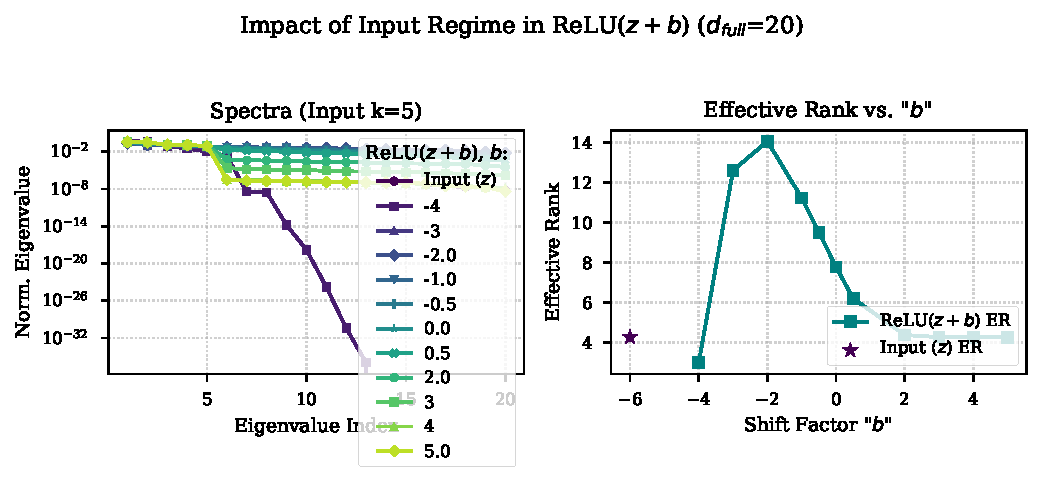
\includegraphics[width=0.7\linewidth]{figures/theory_relu_zb_rank.pdf} % Assuming image is in figures/
    \caption{Effect of input shifting on post-activation effective rank for $h = \mathrm{ReLU}(z+b)$, with rank-deficient $z$ (initial ER=5, $d_{\text{full}}=20$). \textbf{Left:} Normalized eigenvalue spectra of $\mathrm{Cov}(h)$. \textbf{Right:} Effective rank of $\mathrm{Cov}(h)$ vs. shift $b$. Large positive $b$ (making $z+b > 0$) results in affine behavior ($\mathrm{ReLU}(z+b) \approx z+b$), limiting rank recovery. Large negative $b$ causes rank collapse (most outputs are zero). An optimal $b$ (near zero for zero-mean $z$) maximizes non-linear effectiveness and rank expansion.}
    \label{fig:theory_relu_zb_rank}
\end{figure}

Figures~\ref{fig:theory_tanh_az_rank} and \ref{fig:theory_relu_zb_rank} show that inappropriate pre-activation scaling or centering can force Tanh and ReLU into regimes of weak effective non-linearity. This compromises their rank recovery capacity, potentially worsening plasticity loss if representations become increasingly rank-deficient. Controlling pre-activation statistics is thus crucial. Techniques like Batch Normalization (BN) standardize these statistics, guiding activations into their effective non-linear zones, as demonstrated in Figure~\ref{fig:theory_joint_norm_activation_rank}.

\begin{figure}[ht!]
    \centering
    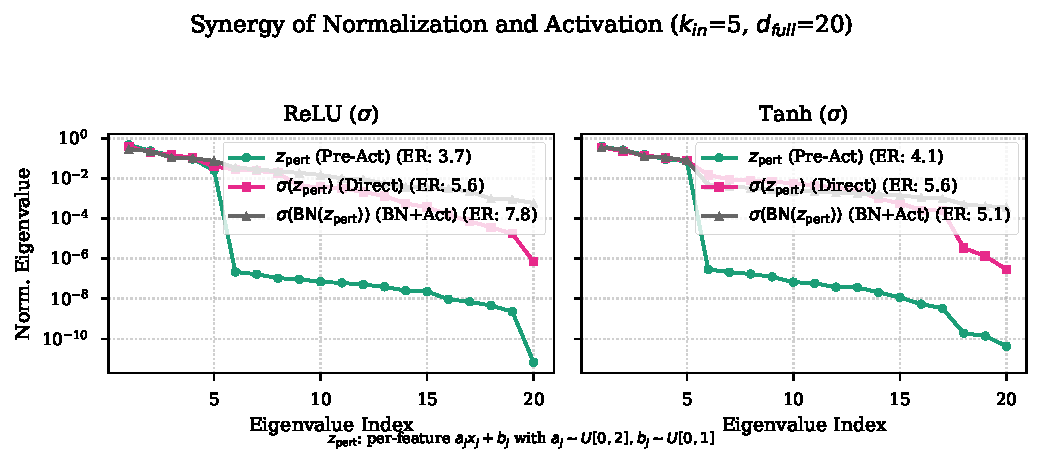
\includegraphics[width=0.7\linewidth]{figures/theory_joint_norm_activation_rank.pdf} % Assuming image is in figures/
    \caption{Synergy of Batch Normalization (BN) with ReLU and Tanh for rank recovery from perturbed inputs $z_{\text{pert}}$ (initial ER=5, $d_{\text{full}}=20$, then per-feature random scaling/shifting). Plots show normalized eigenvalue spectra for $\mathrm{Cov}(\cdot)$ of: (i) $z_{\text{pert}}$ (blue, 'Pre-Act'), (ii) activation on $z_{\text{pert}}$ (orange, 'Direct'), (iii) activation on $\text{BN}(z_{\text{pert}})$ (green, 'BN+Act'). BN before activation (green) consistently restores or enhances effective rank, countering detrimental effects of input perturbations and highlighting BN's role in maintaining effective non-linearity.}
    \label{fig:theory_joint_norm_activation_rank}
\end{figure}

The insights from Proposition~\ref{prop:rank}, supported by these empirical illustrations (Figures~\ref{fig:theory_tanh_az_rank}--\ref{fig:theory_joint_norm_activation_rank}), motivate specific architectural choices and training techniques, discussed next.


\begin{figure}[h!]
    \centering
    % Ensure this figure path and name are correct, e.g., figures/empirical_all_metrics_relu_mnist.pdf
    % Adjust width as needed.
    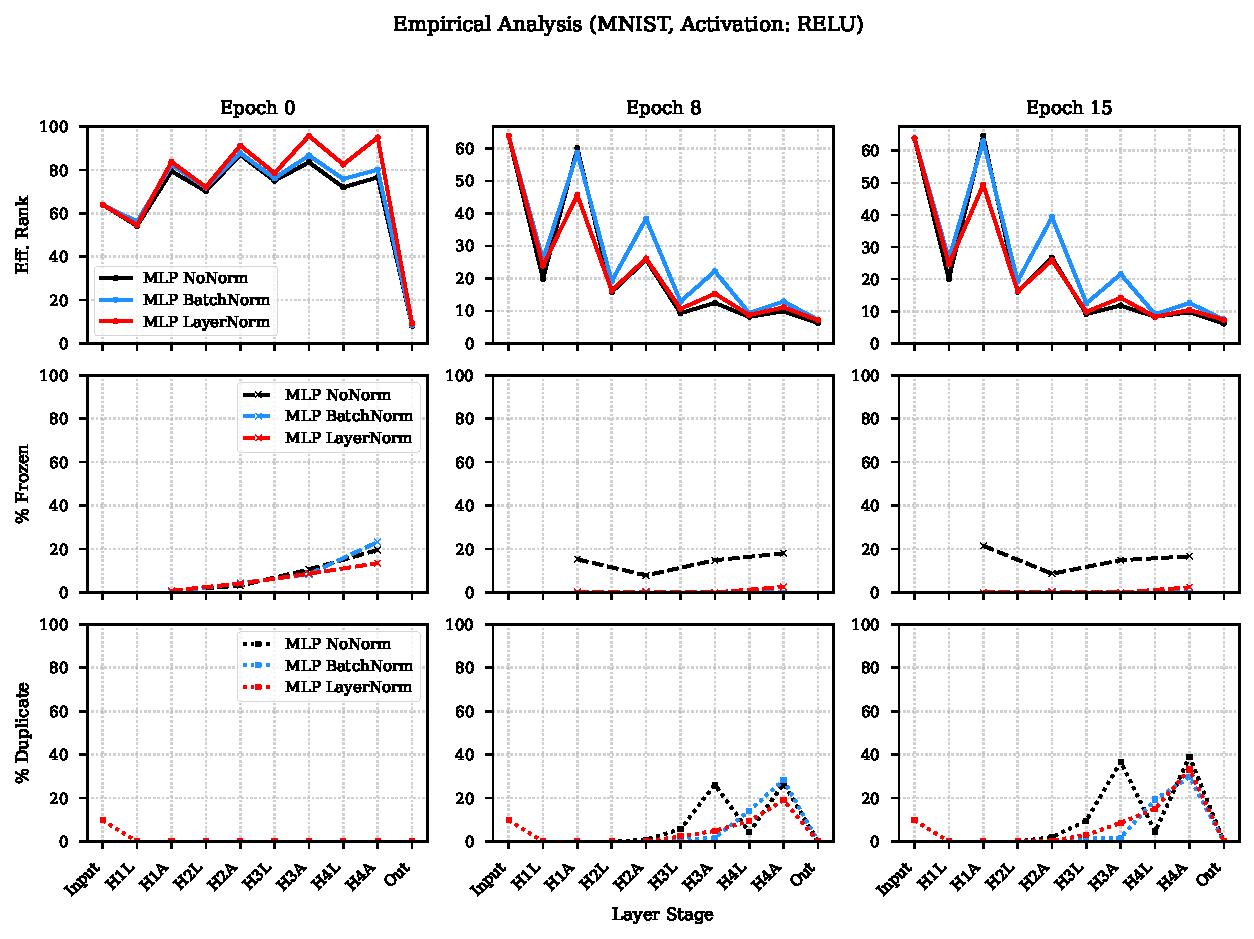
\includegraphics[width=\textwidth]{figures/empirical_all_metrics_ReLU_MNIST.pdf}
    \caption{Comprehensive empirical metrics for an MLP with ReLU activation trained on MNIST, comparing no normalization, Batch Normalization, and Layer Normalization (colors used to distinguish configurations, as per legend within plots). Metrics shown are: (Top Row) Effective Rank, (Middle Row) Percentage of Frozen ReLU Units, and (Bottom Row) Percentage of Duplicate Units. Each column of subplots represents a different training epoch (e.g., early, mid, and late training stages from left to right). Normalization, especially BatchNorm, not only helps maintain higher effective rank (consistent with Figure~\ref{fig:empirical_rank_progression}) but also tends to reduce the percentage of frozen units and duplicate units, particularly in later epochs. This further indicates healthier network dynamics and preserved potential for plasticity when activations are operating in well-conditioned regimes.}
    \label{fig:empirical_all_metrics}
\end{figure}

The trends observed in Figure~\ref{fig:empirical_all_metrics} for effective rank (top row) align with the more detailed epoch-wise progression shown in Figure~\ref{fig:empirical_rank_progression} in the main text. Furthermore, the use of normalization, particularly Batch Normalization, often correlates with a lower percentage of frozen ReLU units (middle row) and duplicate neurons (bottom row) as training progresses. This suggests that by maintaining better-conditioned inputs to activations, normalization not only aids in rank preservation but also mitigates other symptoms associated with the loss of plasticity, such as unit saturation and representational redundancy. These observations further strengthen the argument that architectural choices promoting effective non-linear operation are crucial for sustained learning.



\section{Proofs}
\label{app:proofs}

\begin{proof}[Proof of Proposition~\ref{prop:cloned} (Cloned-unit plasticity loss)]
    Let $\mathcal{G}=(\mathcal{V},\mathcal{E},\mathcal{W})$ be the cloned network and $G=(V,E,W)$ the narrow network, with a partition $\{S_v\}_{v\in V}$ of $\mathcal{V}$. Assume activation functions $f_v$ are identical for all nodes within a partition $S_v$. Let $\mathcal{W}(t)$ be the parameters of $\mathcal{G}$ at time $t$. We need to show that if the initial weights $\mathcal{W}(0)$ satisfy certain cloning conditions, then the gradient flow keeps the parameters within an affine subspace determined by the dynamics of $G$.

    \textbf{Cloning Conditions (Informal):} The weights $\mathcal{W}$ must be initialized such that for any input $x$, (1) all nodes $u, v \in S_k$ have the same activation $h(u)=h(v)$, and (2) for any loss function, all nodes $u, v \in S_k$ receive the same backward error signal $\delta(u)=\delta(v)$. Precise conditions involve relationships between sums of weights connecting partitions, ensuring that the distributed weights in $\mathcal{G}$ effectively replicate the function of the single weights in $G$. For example, for linear networks, we might require $\sum_{u' \in S_u} \mathcal{W}(u', v') = W(u,v)$ for all $v' \in S_v$, and $\sum_{v' \in S_v} \mathcal{W}(u', v') = W(u,v)$ for all $u' \in S_u$, potentially scaled by partition sizes depending on the exact setup.

    \textbf{Forward Cloning Induction:} Assume $h(u') = h_u$ for all $u' \in S_u$ for all partitions $S_u$ up to a certain layer or distance from the input. Consider a node $v' \in S_v$. Its pre-activation is $z(v') = \sum_{S_u \text{ s.t. } (u,v)\in E} \sum_{u' \in S_u} \mathcal{W}(u', v') h(u')$. Due to the induction hypothesis $h(u')=h_u$, this becomes $z(v') = \sum_{S_u} h_u \sum_{u' \in S_u} \mathcal{W}(u', v')$. If the cloning condition ensures $\sum_{u' \in S_u} \mathcal{W}(u', v')$ is constant for all $v' \in S_v$ (equal to $W(u,v)$ possibly scaled), then $z(v')$ is the same for all $v' \in S_v$. Since $f_v$ is the same for all nodes in $S_v$, $h(v') = f_v(z(v'))$ is also constant across $S_v$. By induction, forward activations are cloned.

    \textbf{Backward Cloning Induction:} Assume $\delta(u') = \delta_u$ for all $u' \in S_u$ for all partitions $S_u$ down to a certain layer or distance from the output. Consider a node $v' \in S_v$. Its error signal is $\delta(v') = f'_v(z(v')) \sum_{S_w \text{ s.t. } (v,w)\in E} \sum_{w' \in S_w} \delta(w') \mathcal{W}(v', w')$. By forward cloning $z(v')$ is constant across $S_v$, so $f'_v(z(v'))$ is constant. By induction hypothesis $\delta(w')=\delta_w$. So, $\delta(v') = f'_v(z_v) \sum_{S_w} \delta_w \sum_{w' \in S_w} \mathcal{W}(v', w')$. If the cloning condition ensures $\sum_{w' \in S_w} \mathcal{W}(v', w')$ is constant for all $v' \in S_v$ (equal to $W(v,w)$ possibly scaled), then $\delta(v')$ is constant across $S_v$. By induction, backward error signals are cloned.

    \textbf{Weight Gradient Cloning:} The gradient for a weight $\mathcal{W}(u', v')$ with $u' \in S_u, v' \in S_v$ is $\frac{\partial \Loss}{\partial \mathcal{W}(u', v')} = \delta(v') f'_v(z(v')) h(u')$. Since $h(u')$, $z(v')$, $f'_v(z(v'))$, and $\delta(v')$ are all constant within their respective partitions ($h_u$, $z_v$, $f'_v(z_v)$, $\delta_v$), the gradient is constant for all pairs $(u', v')$ connecting partitions $S_u$ and $S_v$. Let this constant gradient be $g_{uv}$.
    The total gradient for the effective weight $W(u,v)$ in the narrow network corresponds to the sum of these individual gradients (scaled appropriately).
    Let $\mathcal{W}(t) = \mathcal{W}(0) + \Delta\mathcal{W}(t)$. An update step is $\Delta\mathcal{W}(t+\Delta t) = \Delta\mathcal{W}(t) - \eta \nabla \Loss(\mathcal{W}(t))$. Since $\frac{\partial \Loss}{\partial \mathcal{W}(u', v')} = g_{uv}$ for all $u' \in S_u, v' \in S_v$, the change $\Delta\mathcal{W}(u', v')$ is identical for all these weights. This preserves the cloning structure. The evolution of the system is thus driven by the effective gradients $g_{uv}$, which correspond to the gradients of the narrow network $G$. The parameters $\mathcal{W}(t)$ are therefore confined to the affine subspace $\mathcal{W}(0) + \text{span}\{\mathbf{1}_{S_u \times S_v} \mid (u,v) \in E\}$, where $\mathbf{1}_{S_u \times S_v}$ is a matrix with 1s for connections between $S_u$ and $S_v$ and 0s elsewhere. The dimension of this subspace is $|E|$. This manifold is stable because any perturbation that breaks the symmetry would, under gradient descent using only first-order information, be averaged out over the cloned units, reinforcing the symmetric state.
\end{proof}

\begin{proof}
    Let $f:\R\to\R$ be square-integrable w.r.t. $\gamma = \mathcal{N}(0,1)$ and not a polynomial. Let $z \sim \mathcal{N}(0, \Sigma)$ with $\Sigma_{ii}=1$ and $|\Sigma_{ij}| < 1$ for $i \neq j$. We want to show $C = \E[f(z)f(z)^\top]$ is full rank.
    Since $f$ is square-integrable w.r.t. $\gamma$, it has a Hermite expansion $f(x) = \sum_{k=0}^{\infty} b_k \frac{\He_k(x)}{\sqrt{k!}}$, where $\He_k(x)$ are the standard probabilist's Hermite polynomials and $b_k = \E[f(Z) \frac{\He_k(Z)}{\sqrt{k!}}]$ for $Z \sim \mathcal{N}(0,1)$. Since $f$ is not a polynomial, infinitely many $b_k$ must be non-zero. For simplicity, let's use the physicist's convention where $f(x) = \sum_{k=0}^{\infty} c_k \He_k(x)$ with $c_k = \frac{1}{2^k k! \sqrt{\pi}} \int f(x) \He_k(x) e^{-x^2} dx$. Infinitely many $c_k$ are non-zero.

    Mehler's formula \cite{mehler1866ueber, erdelyi1953higher} provides the expectation of products of Hermite polynomials for correlated Gaussian variables. For $(Z_i, Z_j)$ jointly Gaussian with mean 0, variance 1, and correlation $\rho = \Sigma_{ij}$, we have $\E[\He_k(Z_i) \He_l(Z_j)] = \delta_{kl} 2^k k! \rho^k$.

    The $(i, j)$-th entry of the covariance matrix $C$ is $C_{ij} = \E[f(z_i) f(z_j)]$. Substituting the Hermite expansion:
    \begin{align*}
    C_{ij} &= \E\left[ \left( \sum_{k=0}^{\infty} c_k \He_k(z_i) \right) \left( \sum_{l=0}^{\infty} c_l \He_l(z_j) \right) \right] \\
    &= \sum_{k=0}^{\infty} \sum_{l=0}^{\infty} c_k c_l \E[\He_k(z_i) \He_l(z_j)] \\
    &= \sum_{k=0}^{\infty} c_k^2 \E[\He_k(z_i) \He_k(z_j)] \quad (\text{using orthogonality } \delta_{kl}) \\
    &= \sum_{k=0}^{\infty} c_k^2 (2^k k!) (\Sigma_{ij})^k
    \end{align*}
    Let $a_k = c_k^2 (2^k k!)$. Since infinitely many $c_k \neq 0$, infinitely many $a_k > 0$. The matrix $C$ can be written as $C = \sum_{k=0}^{\infty} a_k \Sigma^{\odot k}$, where $\Sigma^{\odot k}$ is the element-wise $k$-th power (Hadamard power) of the pre-activation covariance matrix $\Sigma$.

    We know $\Sigma$ is positive semidefinite (as it's a covariance matrix) and by assumption $\Sigma_{ii}=1$ and $|\Sigma_{ij}|<1$ for $i \neq j$. $\Sigma^{\odot 0}$ is a matrix of all ones (rank 1). $\Sigma^{\odot 1} = \Sigma$. For $k \ge 1$, if $\Sigma$ is positive definite, then $\Sigma^{\odot k}$ is also positive definite (Schur product theorem). Even if $\Sigma$ is only positive semidefinite, as $k$ increases, the off-diagonal elements $(\Sigma_{ij})^k$ decay towards zero since $|\Sigma_{ij}|<1$. By Gershgorin circle theorem arguments, for large enough $k$, the matrix $\Sigma^{\odot k}$ becomes strictly diagonally dominant and thus positive definite, provided $\Sigma$ doesn't represent linearly dependent variables (which is implied by $|\Sigma_{ij}|<1$).

    Since $C$ is a sum of positive semidefinite matrices ($\Sigma^{\odot k}$ for $k \ge 1$, scaled by non-negative $a_k$), and at least one $a_k > 0$ corresponds to a positive definite $\Sigma^{\odot k}$ (for $k \ge 1$, assuming $\Sigma$ is not degenerate), the resulting matrix $C$ will be positive definite, hence full rank. The only exception is if the original $z_i$ were linearly dependent such that $\Sigma$ was rank-deficient in a way that persists through the Hadamard powers (e.g., if $z_i = z_j$ or $z_i = -z_j$, making $\Sigma_{ij}=1$ or $\Sigma_{ij}=-1$, violating the assumption).
\end{proof}


\section{Corollary on architectural extensions}
The framework, particularly Proposition~\ref{prop:cloned} on cloned units, can be conceptually extended to cover common architectural components beyond simple MLPs:
\begin{itemize}
    \item \textbf{Bias Terms:} Bias terms can be incorporated by viewing them as weights connected to an input unit that always has an activation of 1. The cloning analysis applies directly if the bias terms within a partition $S_v$ are also identical initially and receive identical gradient updates.
    \item \textbf{Convolutional Neural Networks (CNNs):} While Proposition~\ref{prop:cloned} is stated for individual units, it can be adapted to CNNs by considering entire channels as the units being potentially cloned. If multiple channels in a layer compute identical feature maps due to symmetric initialization and subsequent updates, they form a cloned-channel manifold, reducing the effective representational capacity similar to the MLP case.
    \item \textbf{Normalization Layers (LayerNorm, RMSNorm) and Softmax:} These layers involve interactions across multiple units/features within a layer, unlike simple element-wise activations. The cloning proposition doesn't directly apply in its current form. However, the principle of dimensionality collapse can still manifest. If the inputs to such a layer belong to partitions $\{S_i\}$ where activations within each partition are identical ($h_i$), the normalization statistics (mean, variance) or softmax denominators can be computed using weighted contributions from these partitions. For example, for LayerNorm, the mean $\mu$ and variance $\sigma^2$ over $n$ inputs partitioned into $m$ sets $S_i$ would be $\mu = \frac{1}{n}\sum_{i=1}^m |S_i| h_i$ and $\sigma^2 = \frac{1}{n}\sum_{i=1}^m |S_i| (h_i - \mu)^2$. The output for a unit in partition $S_j$ would be $(h_j - \mu) / \sqrt{\sigma^2 + \epsilon}$. Similarly for Softmax, the output for a unit in $S_j$ would be $e^{h_j} / (\sum_{i=1}^m |S_i| e^{h_i})$. If the parameters feeding into these layers maintain the cloning structure, the outputs will also be cloned, and the dynamics remain trapped, albeit the manifold definition might become more complex than a simple affine subspace. An ad-hoc low-dimensional equivalent model capturing this behavior can be formulated.
\end{itemize}

The cloning result is also robust to common optimization algorithm variations:
\begin{itemize}
    \item \textbf{Mini-batch SGD:} Using mini-batches averages gradients over multiple samples. Since the cloning structure holds for the gradient of each sample, the averaged gradient will also exhibit the same block-wise constant structure across partitions. Thus, mini-batch SGD does not break the symmetry.
    \item \textbf{Momentum / Adam:} Optimizers like SGD with Momentum or Adam maintain running averages of past gradients (first moment) and squared gradients (second moment). If the gradients $\nabla\Loss(\mathcal{W})$ possess the cloning structure, then the first and second moment estimates will also inherit this structure. Consequently, the parameter updates derived from these statistics will preserve the cloning symmetry, and the trajectory remains confined to the manifold.
\end{itemize}
These extensions suggest that the core mechanisms of plasticity loss identified are likely relevant across a cloned range of modern deep learning architectures and optimizers.

\section{Experimental Setup}

\subsection{Metrics}

\section{Additional experimental evidence}


\begin{figure}[h!]
    \centering
    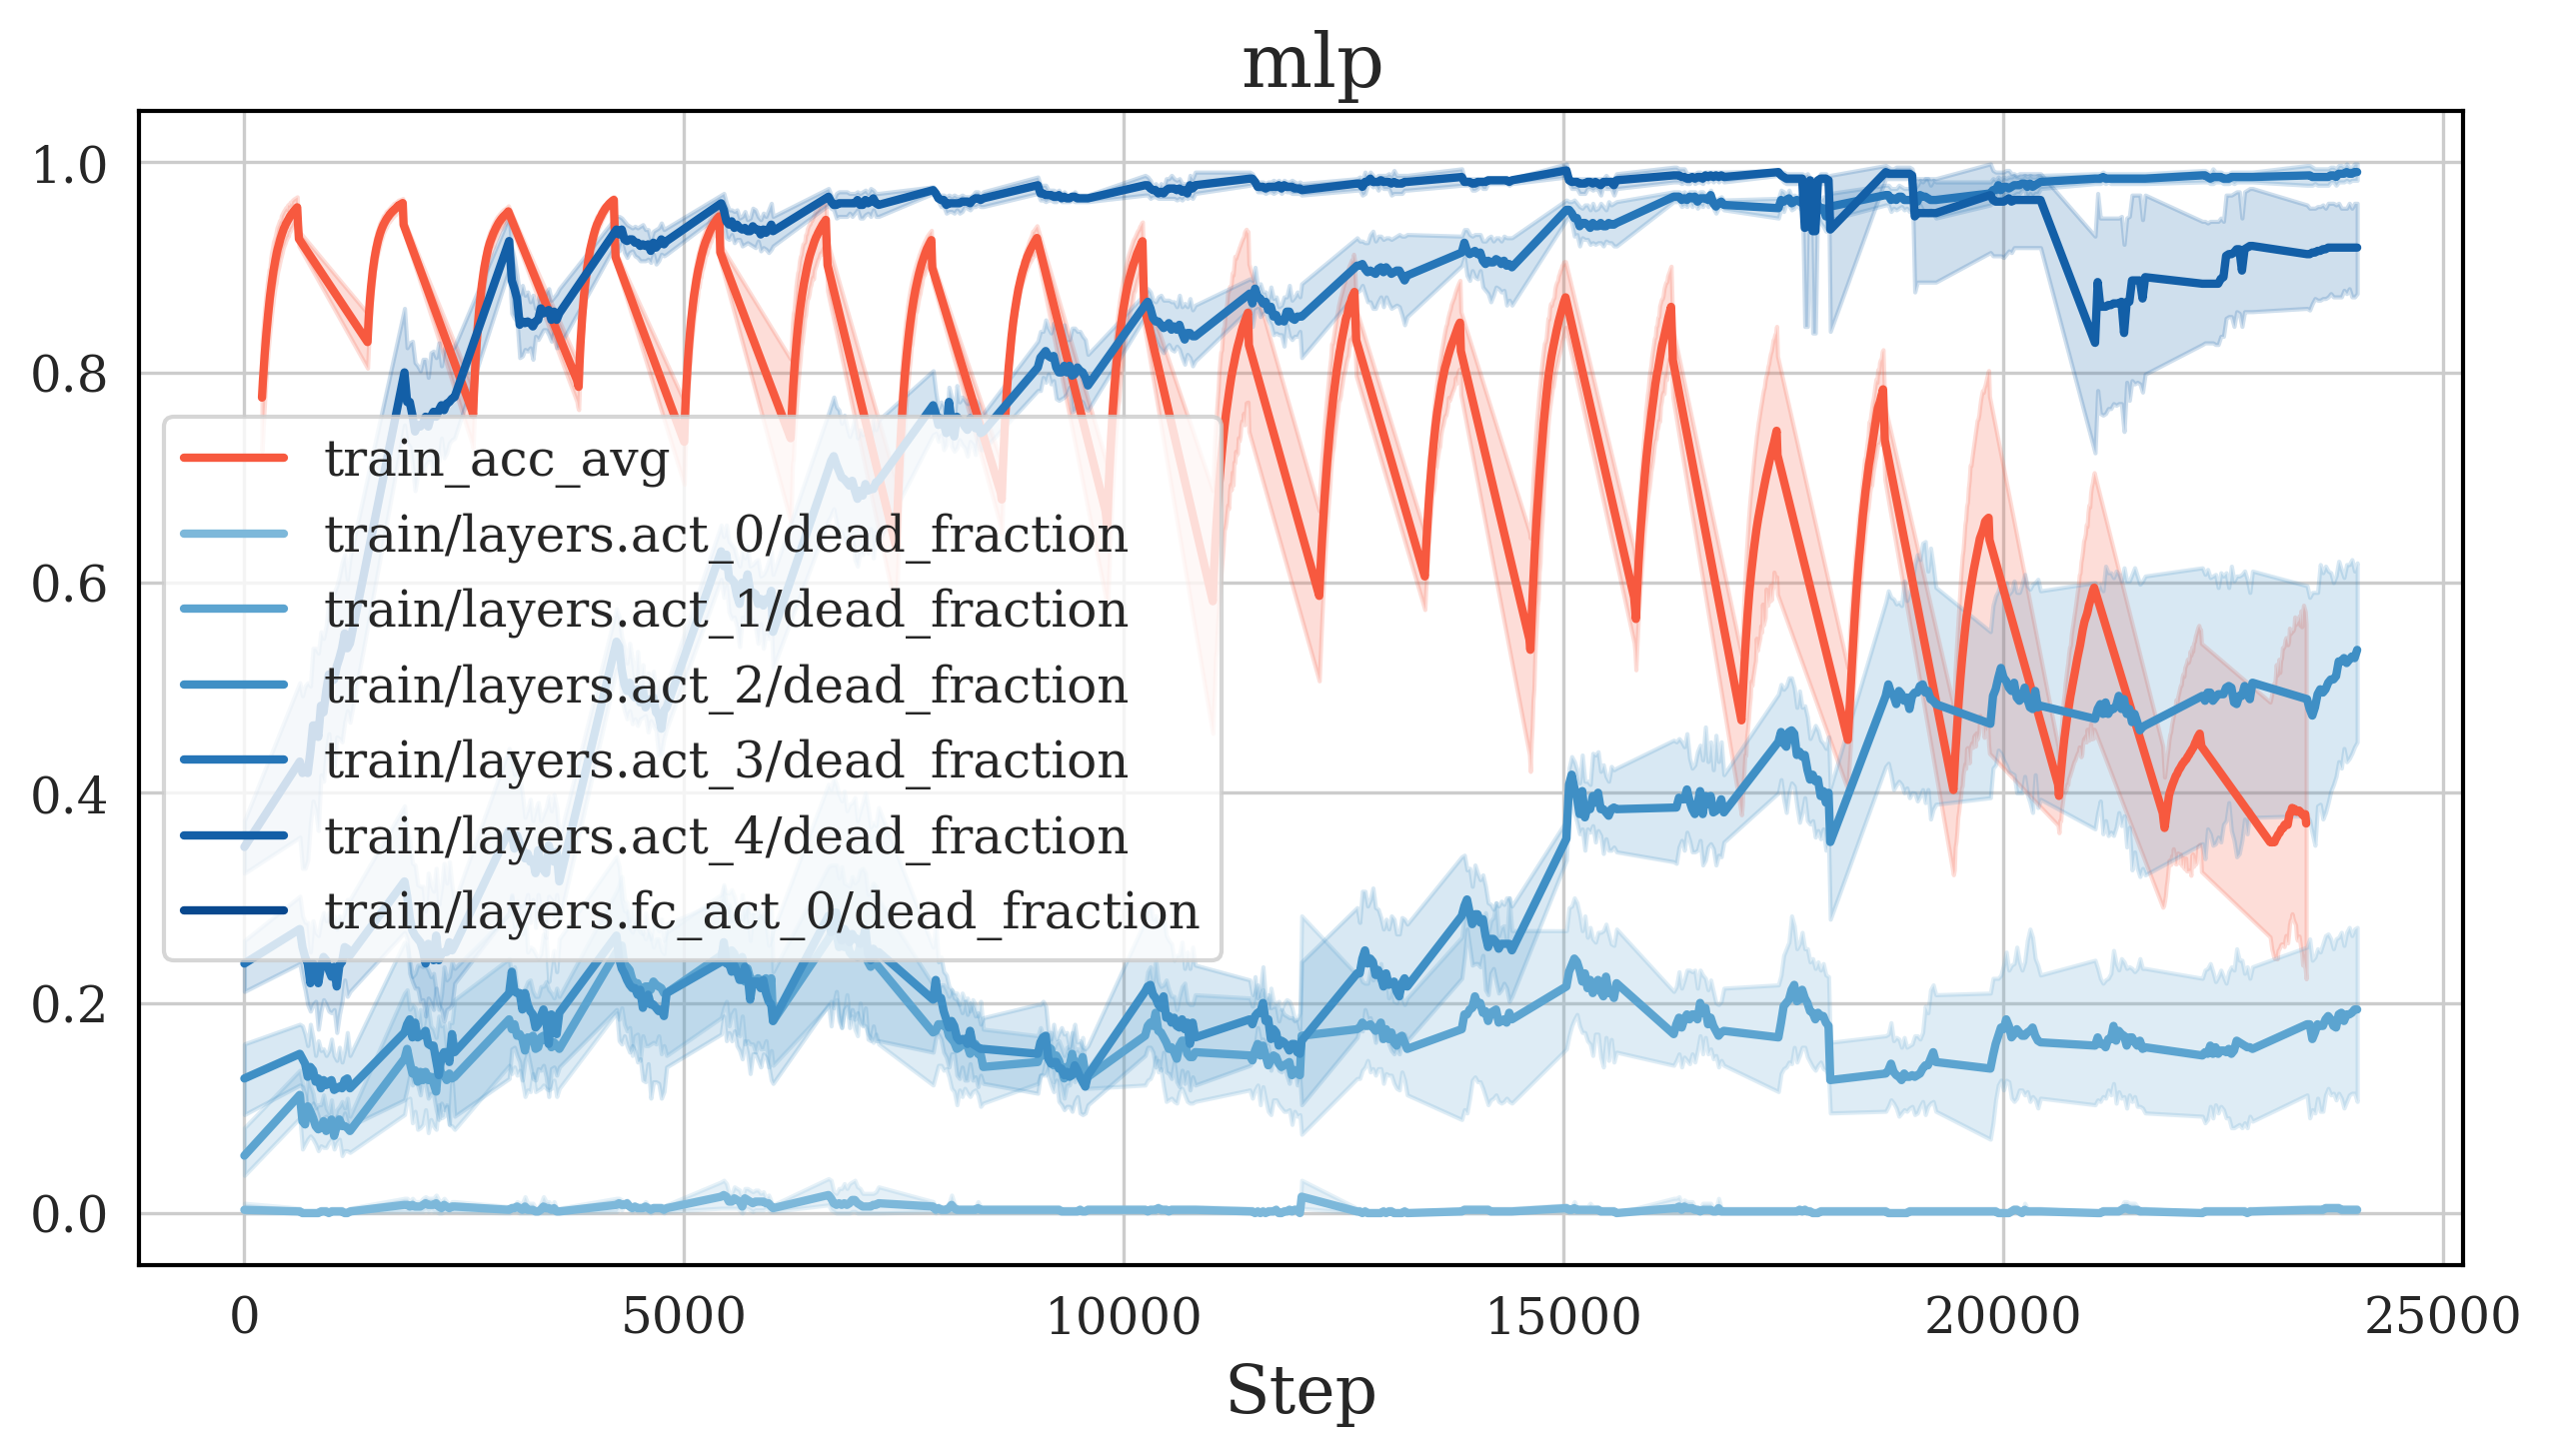
\includegraphics[width=0.45\linewidth]{paper/images/dead_frac_mlp_layer_detail.png}
    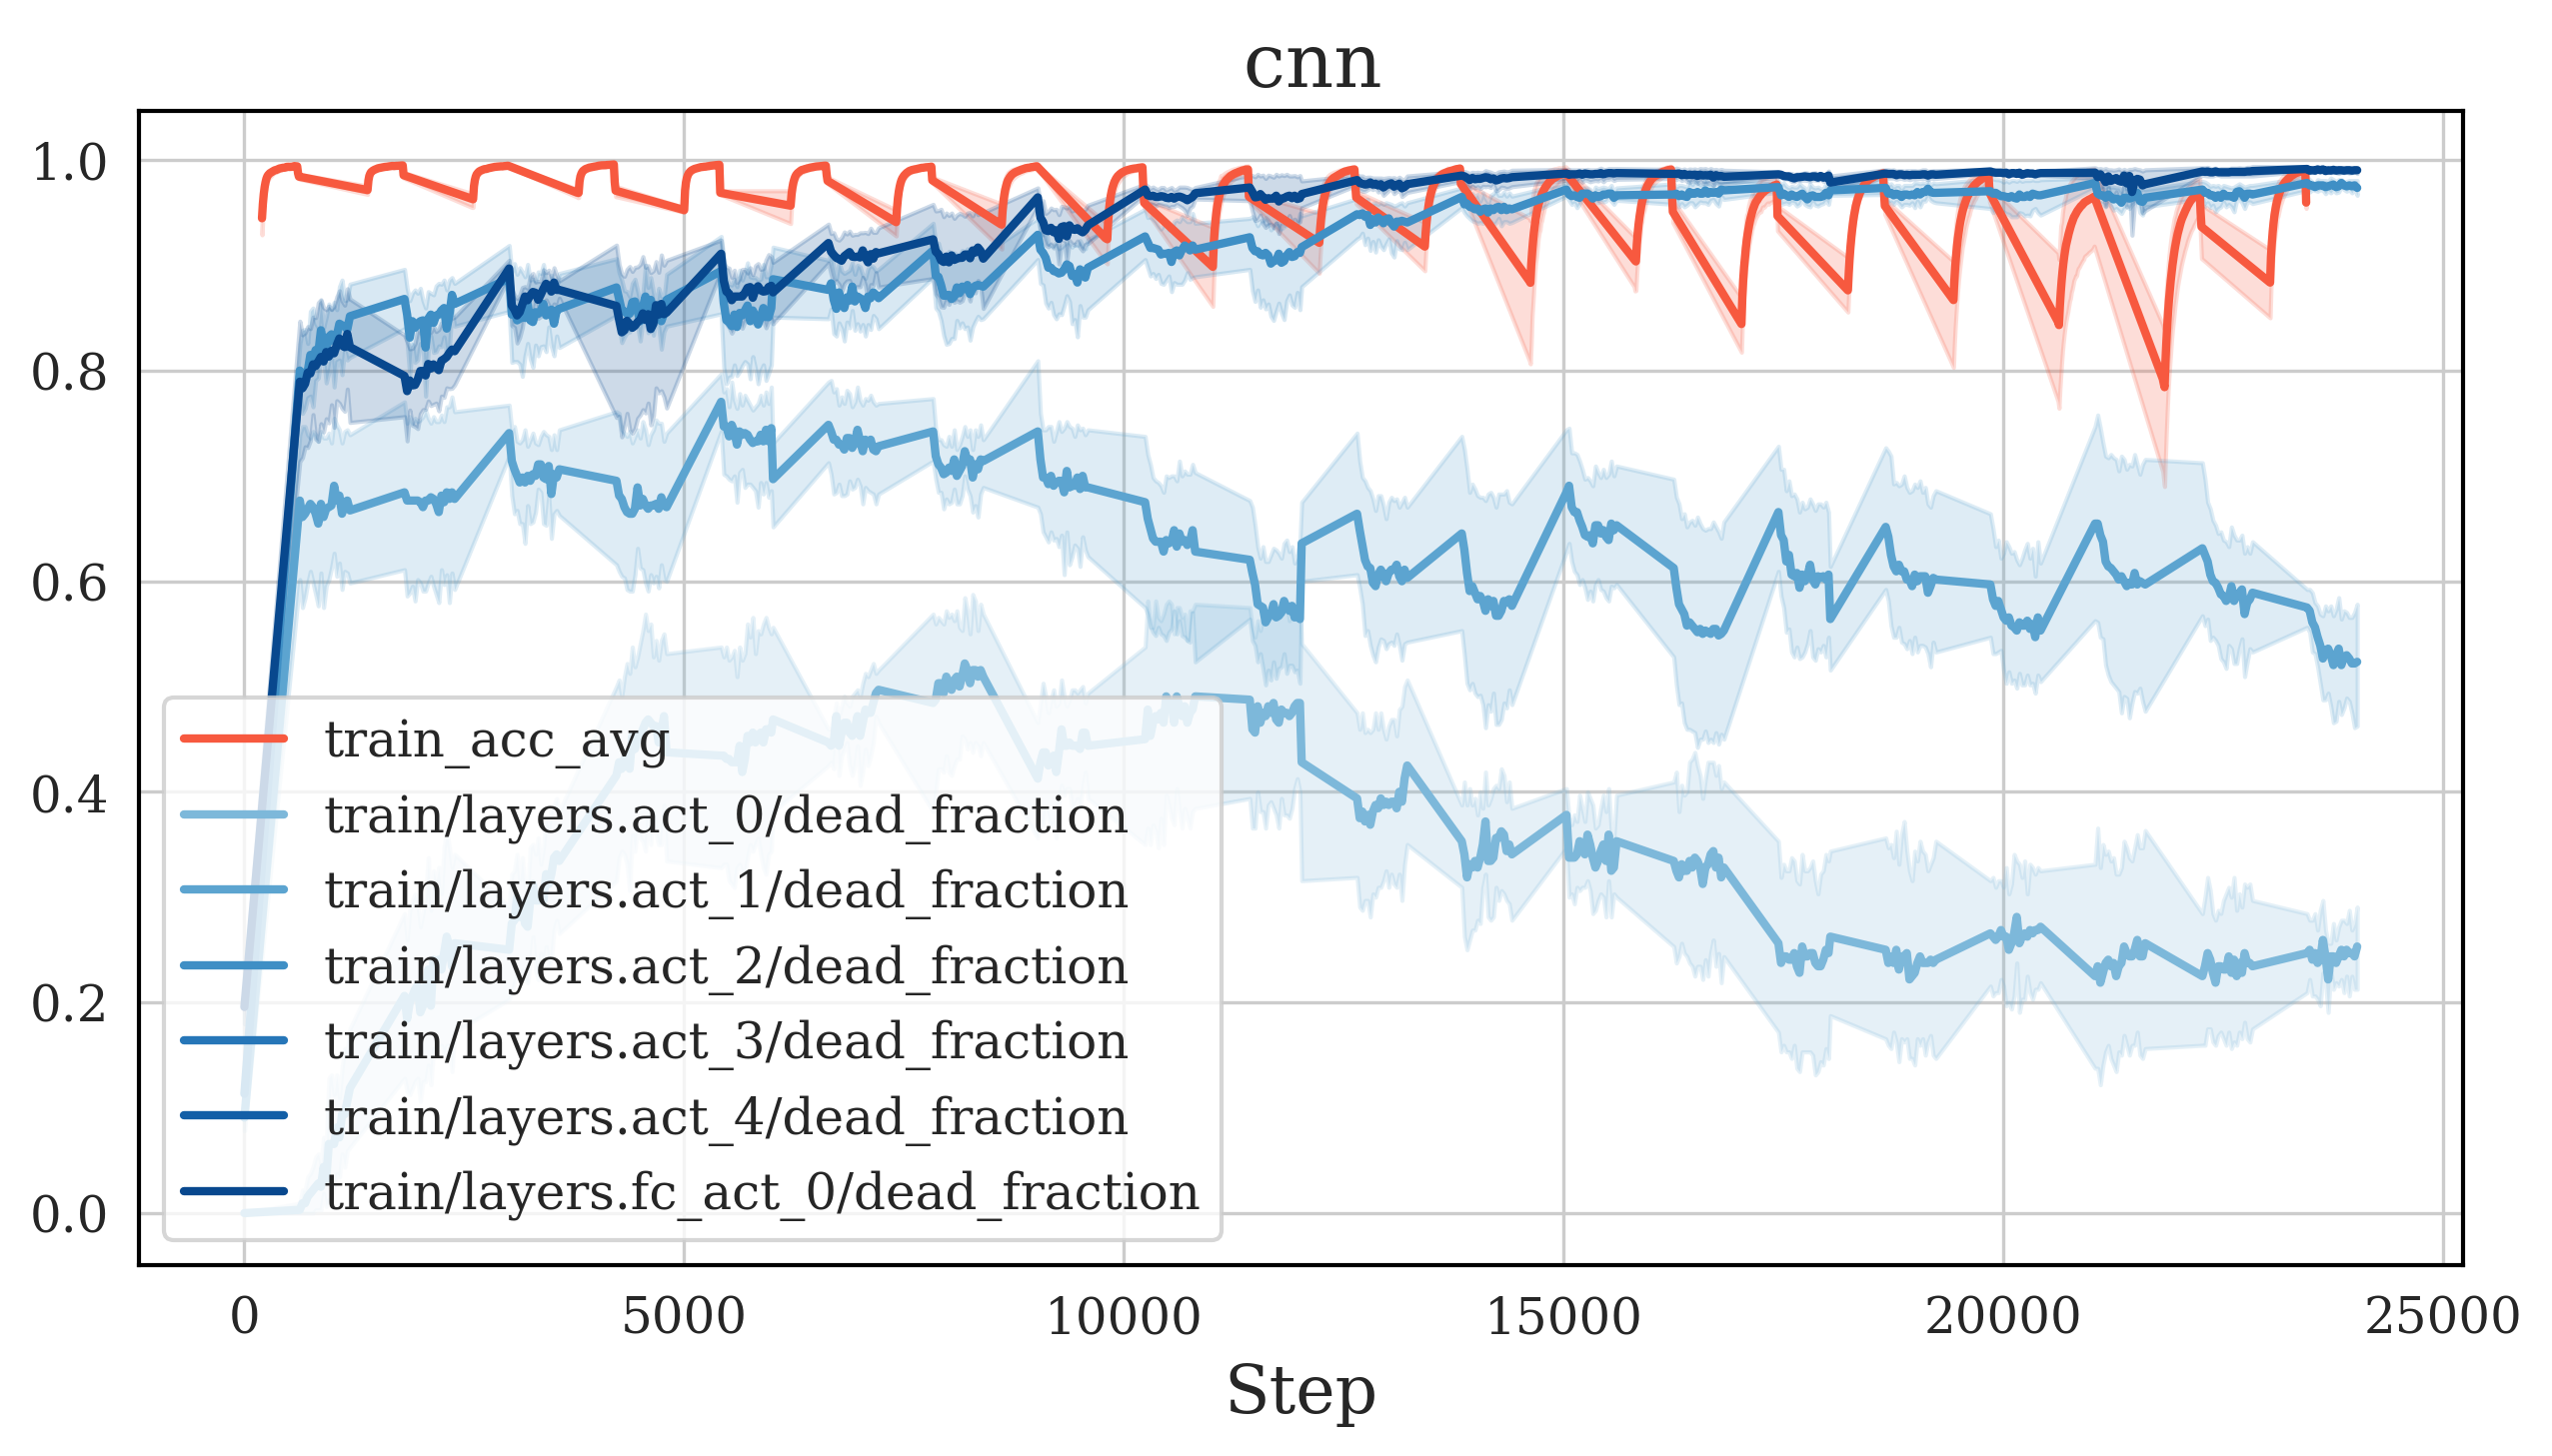
\includegraphics[width=0.45\linewidth]{paper/images/dead_frac_cnn_layer_detail.png}
    \caption{(Placeholder figure, not final) No normalization and no dropout. Detail by layers.}
    \label{fig:DeadReLUs-LoP}
\end{figure}
\newpage

\section*{NeurIPS Paper Checklist}
\begin{enumerate}
\item {\bf Claims}
    \item Answer: \answerYes{}
    \item Justification: The claims in the abstract and introduction accurately reflect the paper's contributions on loss of plasticity in neural networks, linking it to specific mechanisms (saturation, cloning) and proposing a dynamical systems framework.

\item {\bf Limitations}
    \item Answer: \answerYes{}
    \item Justification: Limitations are discussed in the Discussion section (Section 7), acknowledging open questions regarding non-linear manifolds, advanced optimizers, PEFT interactions, and the need for more sophisticated continual randomization schemes.

\item {\bf Theory assumptions and proofs}
    \item Answer: \answerYes{}
    \item Justification: All theoretical results (propositions, corollary) state their assumptions clearly. Complete proofs are provided in Appendix~\ref{app:proofs}.

\item {\bf Experimental result reproducibility}
    \item Answer: \answerNA{} % Changed from Yes to NA as experiments are planned
    \item Justification: Section~\ref{sec:experiments} outlines planned experiments. Details on specific datasets, architectures, hyperparameters, and evaluation protocols would be provided with the results in a final version, enabling reproducibility. Code would also be released.

\item {\bf Open access to data and code}
    \item Answer: \answerNA{} % Changed from Yes to NA as experiments are planned
    \item Justification: Code and experimental configurations related to the planned experiments in Section~\ref{sec:experiments} will be made available upon completion and acceptance. Standard datasets (e.g., CIFAR, ImageNet variants) will be used.

\item {\bf Experimental setting/details}
    \item Answer: \answerNA{} % Changed from Yes to NA
    \item Justification: Section~\ref{sec:experiments} provides a high-level plan. Detailed experimental settings (architectures, optimizers, learning rates, task sequences, specific metrics implementations) will be included when reporting results.

\item {\bf Experiment statistical significance}
    \item Answer: \answerNA{} % Changed from Yes to NA
    \item Justification: Methods for ensuring statistical significance (e.g., multiple runs with different random seeds, reporting means and standard deviations/errors) will be employed and detailed when presenting the results from Section~\ref{sec:experiments}.

\item {\bf Experiments compute resources}
    \item Answer: \answerNo{}
    \item Justification: Details about computational resources (e.g., GPU types, number, training times) for the planned experiments will be added in the final version presenting the empirical results.

\item {\bf Code of ethics}
    \item Answer: \answerYes{}
    \item Justification: The research aims to understand fundamental AI capabilities and limitations, adhering to ethical research practices. It does not involve sensitive data or high-risk applications directly. Conforms to the NeurIPS Code of Ethics.

\item {\bf Broader impacts}
    \item Answer: \answerYes{}
    \item Justification: Section 8 discusses potential positive impacts (more robust, adaptive AI) and negative societal consequences (unpredictability, control issues), aligning with the requirement to address broader impacts.

\item {\bf Safeguards}
    \item Answer: \answerNA{}
    \item Justification: This paper presents a theoretical framework and planned experiments. It does not release new models or datasets with immediate potential for misuse. Safeguards related to potential future applications are discussed in the Broader Impacts section.

\item {\bf Licenses for existing assets}
    \item Answer: \answerNA{} % Changed from Yes to NA
    \item Justification: The planned experiments intend to use standard, publicly available datasets (e.g., CIFAR, ImageNet) which have permissive licenses for research use. This will be confirmed and stated in the final version.

\item {\bf New assets}
    \item Answer: \answerNA{} % Changed from Yes to NA
    \item Justification: Code developed for the experiments will be released with appropriate documentation and an open-source license upon publication.

\item {\bf Crowdsourcing and research with human subjects}
    \item Answer: \answerNA{}
    \item Justification: This research is purely theoretical and computational, involving no human subjects or crowdsourcing.

\item {\bf Institutional review board (IRB) approvals or equivalent for research with human subjects}
    \item Answer: \answerNA{}
    \item Justification: Not applicable as no human subjects are involved.

\item {\bf Declaration of LLM usage}
    \item Answer: \answerNA{}
    \item Justification: No LLMs were used in the development of the core theoretical methods or planned experiments presented in this research. (Note: The generation of this report text involved an LLM based on the provided draft and research snippets, but the research content itself does not rely on LLMs).
\end{enumerate}
\end{document}
